\documentclass[14pt,a4paper,oneside]{book}

\usepackage[utf8]{inputenc}
\usepackage[T1]{fontenc}
\usepackage[brazil]{babel}

\usepackage{enumitem} 
\usepackage{csquotes} 
\usepackage{natbib}   
 
\usepackage{extsizes}
\usepackage{setspace}
\onehalfspacing
\usepackage{anyfontsize}
\fontsize{14pt}{16pt}\selectfont
\usepackage{fancyvrb} 

\usepackage[scaled=0.9]{inconsolata}

\usepackage{hyphenat}
\hyphenation{chat-bot cha-tbots in-te-li-gên-cia ar-ti-fi-cial}

\usepackage{rotating}

\usepackage{geometry} 
\geometry{
  left=2cm, % Aumente a margem esquerda para caber as notas
  right=2cm, % Margem direita menor, já que não terá notas
  bottom=2cm, % Margem direita menor, já que não terá notas
  marginparwidth=2.5cm, % Largura das notas
  marginparsep=0.5cm % Separação entre texto e nota
}

% \makeatletter
% \renewcommand{\verbatim@font}{\ttfamily\footnotesize}
% \makeatother

\usepackage{marginnote}
\reversemarginpar
\renewcommand*{\marginfont}{\color{blue}}

\usepackage{tikz}
\usetikzlibrary{trees} 

\usepackage{lmodern}
\usepackage{graphicx}
\usepackage{amsmath,amssymb}
\usepackage{float}
\usepackage{charter}
\usepackage{xcolor}   
\usepackage[
    colorlinks=true,
    linkcolor=blue,   
    citecolor=blue,  
    urlcolor=blue  
]{hyperref}

\usepackage{listings}

\lstset{
    language=Python,
    basicstyle=\ttfamily\small,
    keywordstyle=\color{blue}\bfseries,
    stringstyle=\color{red},
    commentstyle=\color{green!50!black},
    numbers=left,
    numberstyle=\tiny,
    stepnumber=1,
    numbersep=5pt,
    showspaces=false,
    showstringspaces=false,
    frame=single,
    breaklines=true,
    breakatwhitespace=true,
    tabsize=4,
	literate={á}{{\'a}}1 {ã}{{\~a}}1 {é}{{\'e}}1 {è}{{\`{e}}}1 {ê}{{\^{e}}}1 {ë}{{\¨{e}}}1 {É}{{\'{E}}}1 {Ê}{{\^{E}}}1 {û}{{\^{u}}}1 {ú}{{\'{u}}}1 {â}{{\^{a}}}1 {à}{{\`{a}}}1 {á}{{\'{a}}}1 {ã}{{\~{a}}}1 {Á}{{\'{A}}}1 {Â}{{\^{A}}}1 {Ã}{{\~{A}}}1 {ç}{{\c{c}}}1 {Ç}{{\c{C}}}1 {õ}{{\~{o}}}1 {ó}{{\'{o}}}1 {ô}{{\^{o}}}1 {Õ}{{\~{O}}}1 {Ó}{{\'{O}}}1 {Ô}{{\^{O}}}1 {î}{{\^{i}}}1 {Î}{{\^{I}}}1 {í}{{\'{i}}}1 {Í}{{\~{Í}}}1,
}

%%%%%%%%%%%%%%%%%
%%%%%CONFIG%%%%%%
%%%%%%%%%%%%%%%%%

% \title{Chatbot Book}
% \author{Giseldo Neo (versão beta)}
% \date{\today}

\begin{document}

\newpage

% \begin{figure}[p]
% 	\centering
% 	\vspace*{-4cm} % Preenche o espaço vertical no topo
% 	\hspace*{-3.8cm} % Compensa a margem esquerda
% 	\makebox[\textwidth]{
% 	  
\includegraphics[width=1.00\paperwidth,height=1.0\paperheight,keepaspectratio=true]{./fig/capa.png}
% 	}
% \end{figure}

\clearpage            
\thispagestyle{empty} 
\begin{figure}[p]
	\centering
	\vspace*{-1.5in} % Ajusta a posição vertical
	\hspace*{-0.82in} % Ajusta a posição horizontal
	
\includegraphics[width=\paperwidth, height=\paperheight]{capa.pdf}
\end{figure}
\clearpage     

\newpage

\tableofcontents
\newpage

%%%%%%%%%%%%%%%%
%%%%CAPITULO%%%%
%%%%%%%%%%%%%%%%

\chapter{Chatbots: Definições e Contexto}

\section{Introdução}

% \marginnote{Definição}
Um chatbot é um programa de computador que simula uma conversa humana, geralmente utilizando texto ou áudio. Eles oferecem respostas diretas a perguntas e auxiliam em diversas tarefas, servindo tanto para conversas gerais quanto para ações específicas, como abrir uma conta bancária.

% \marginnote{Origem do termo}
Embora o chatbot ELIZA \cite{Weizenbaum1996} seja frequentemente considerado um dos primeiros exemplos de software conversacional, o termo ``chatbot'' ainda não era utilizado na época de sua criação. 
O termo ``chatterbot'', sinônimo de ``chatbot'', foi popularizado por Michael Mauldin em 1994, ao descrever seu programa JULIA \cite{Mauldin1994}. 
Publicações acadêmicas, como os anais da \textit{Virtual Worlds and Simulation Conference} de 1998 \cite{Jacobstein1998}, também ajudaram a consolidar o uso do termo.

% \marginnote{ELIZA}
O ELIZA, criado em 1966 por Joseph Weizenbaum,  representou um experimento revolucionário na interação humano-computador \cite{Weizenbaum1996}. Seu roteiro (ou script)  mais famoso, DOCTOR, imitava rudimentarmente um psicoterapeuta, utilizando correspondência de padrões simples. Por exemplo, quando um usuário inseria a frase “Estou triste”, o ELIZA respondia “Por que você está triste hoje?”, reformulando a entrada como uma pergunta. 
Seu funcionamento baseia-se em um conjunto de regras que lhe permitem analisar e compreender a linguagem humana de forma limitada e aproximada. 

Esse tipo de aplicação do ELIZA em simular um psicólogo muito rudimentar da técnica rogeriana adequou-se bem a esse tipo de diálogo pois dependia de pouco conhecimento sobre o ambiente externo. As regras no script DOCTOR permitiam que o programa respondesse ao usuário com outras perguntas ou simplesmente refletisse a afirmação original. 
O ELIZA não possuía uma real ``compreensão'' da linguagem humana; ele apenas utilizava palavras-chave e manipulava frases para que a interação parecesse natural. Uma descrição detalhada do funcionamento do ELIZA, com exemplos em Python, será apresentada em seções posteriores deste livro.

% \marginnote{ChatGPT}
Outro chatbot famoso é o ChatGPT da OpenAI. 
Ele é um modelo de linguagem capaz de gerar texto muito semelhante ao criado por humanos. 
Ele utiliza redes neurais, com aprendizagem profunda, para gerar sentenças e parágrafos com base nas entradas e informações fornecidas. 
Ele produz textos com relativa coerência, responde perguntas, traduz e resume textos. 
Contudo, o ChatGPT não possui consciência nem a capacidade de compreender contexto ou emoções. 

O chatGPT é um exemplo de Modelo de Linguagem Grande (em inglês Large Language Model - LLM), baseado na arquitetura Transformers, introduzida em 2017 \cite{Vaswani2017}. 
Modelos deste tipo são treinados com terabytes de texto, utilizando mecanismos de autoatenção que avaliam a relevância de cada palavra em uma frase. 
Ao contrário das regras manuais do ELIZA, os LLMs extraem padrões linguísticos a partir da vasta quantidade de dados com que a rede neural foi treinada.

% \marginnote{Tipo Conversacional}
Esses dois chatbots, ELIZA e ChatGPT, são bons representantes do tipo de chatbot \textbf{conversacional}. 
Apesar de terem surgido com décadas de diferença — ELIZA em 1966 e ChatGPT em 2022 — e de diferirem bastante na forma como geram suas respostas, ambos compartilham semelhanças em seu objetivo: conversar sobre determinado assunto ou responder perguntas, mantendo o usuário em um diálogo fluido quando necessário. 
Chatbots com essas características podem ser agrupados, de acordo com o objetivo, como chatbots conversacionais e são utilizados para interagir sobre assuntos gerais.

% \marginnote{Tipo Orientado a tarefas} 
Outro tipo de chatbot classificado em relação ao objetivo é o chatbot \textbf{orientado a tarefas}. 
Os chatbots orientados a tarefas executam ações específicas, como abrir uma conta bancária ou pedir uma pizza. 
Geralmente, as empresas disponibilizam chatbots orientados a tarefas para seus usuários, com regras de negócio embutidas na conversação e com fluxos bem definidos. 
Normalmente, não se espera pedir uma pizza e, no mesmo chatbot, discutir os estudos sobre Ética do filósofo Immanuel Kant (embora talvez haja quem queira). 

Essas duas classificações, conversacional e orientado a tarefas  (Figura~\ref{fig:tipo}), ainda não são suficientes para uma completa classifição. 
Existem outras classificações que serão discutidas em seções posteriores. Além disso, uma abordagem híbrida, unindo funções dee  chatbots do tipo conversacional e orientado a tarefas, vem sendo utilizada para atender as necessidades dos usuários. 

\begin{figure}[!htb]
	\centering
	\caption{Classificação dchatbots por objetivo.}
	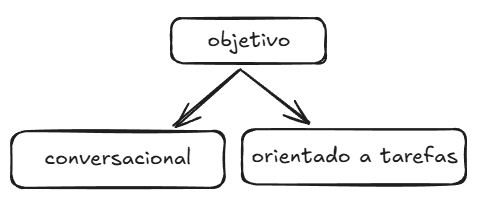
\includegraphics[width=0.9\linewidth]{./fig/tipo_objetivo.png}
	\label{fig:tipo}
\end{figure}

A popularidade dos chatbots tem crescido significativamente em diversos domínios de aplicação \cite{B2020, Klopfenstein2017, Sharma2020}. 
Essa tendência é corroborada pelo aumento do interesse de busca pelo termo ``chatbots'', conforme análise de dados do Google Trends no período entre 2020 e 2025 (Figura~\ref{fig:trends}). 
Nesta figura, os valores representam o interesse relativo de busca ao longo do tempo, onde 100 indica o pico de popularidade no período analisado e 0 (ou a ausência de dados) indica interesse mínimo ou dados insuficientes.

\begin{figure}[!htbp]
	\centering
	\caption{Evolução do interesse de busca pelo termo ``chatbot'' (Google Trends, 2020-2025).}
	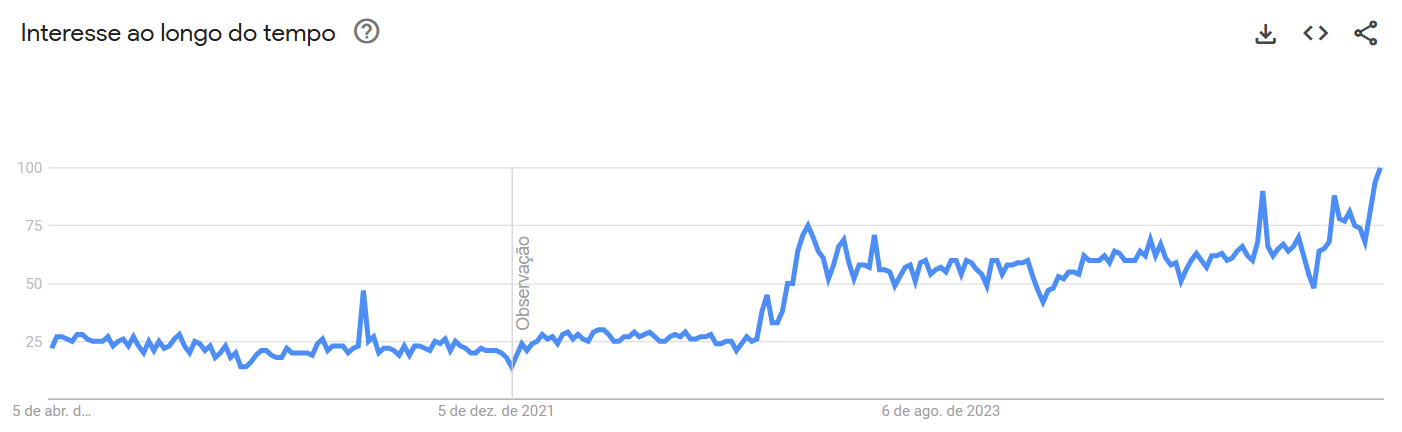
\includegraphics[width=1\linewidth]{./fig/trends.png}
	\label{fig:trends}
	{\footnotesize Fonte: Google Trends acesso em 05/04/2025} % Sugestão: Adicionar a fonte e data de acesso para dados do Trends.
\end{figure}

\section{Agentes}

% \marginnote{Agente}
As definições de chatbot e agentes são usadas indiscriminadamente e podem confundir um pouco. Vamos a uma definição mais precisa.
Um chatbot é um programa computacional projetado para interagir com usuários por meio de linguagem natural. 
Por outro lado, o conceito de agente possui uma definição mais ampla. Um agente trata-se de uma entidade computacional que percebe seu ambiente por meio de sensores e atua sobre esse ambiente por meio de atuadores \cite{Russel2013}. 
A Figura~\ref{fig:agente} ilustra uma arquitetura conceitual de alto nível para um agente.

\begin{figure}[!htb]
	\centering
	\caption{Arquitetura conceitual de um agente.}
	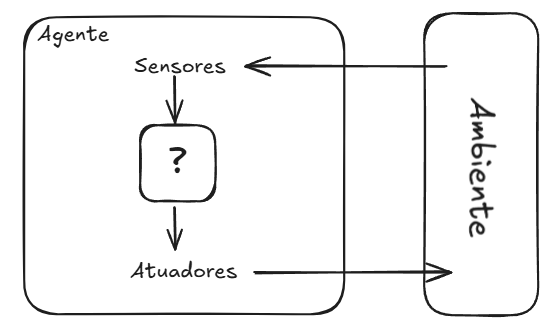
\includegraphics[width=0.7\linewidth]{./fig/original_agente.png}
	\label{fig:agente}
	{\footnotesize \centering

		Fonte: Adaptado de \cite{Russel2013}}
\end{figure}

Nesse contexto, um chatbot (Figura~\ref{fig:chatbot}) pode ser considerado uma instanciação específica de um agente, cujo propósito primário é a interação conversacional em linguagem natural.

\begin{figure}[!htb]
	\centering
	\caption{Representação esquemática de um chatbot.}
	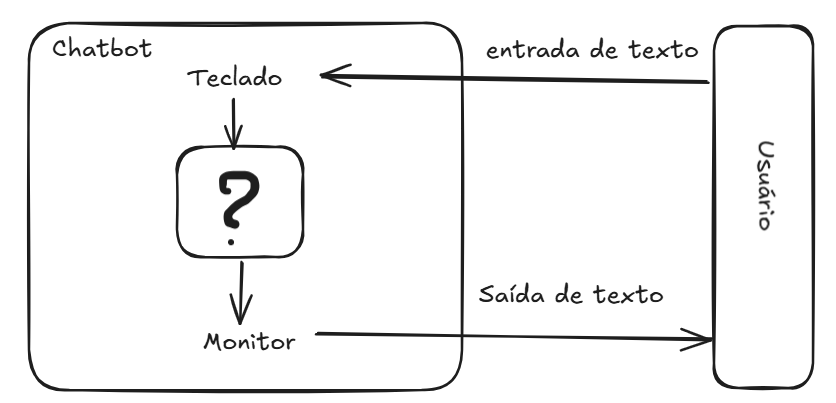
\includegraphics[width=0.7\linewidth]{./fig/chatbot.png}
	\label{fig:chatbot}

\end{figure}

Com o advento de modelos de linguagem, como os baseados na arquitetura \textit{Generative Pre-trained Transformer} (GPT), a exemplo do ChatGPT, observou-se uma recontextualização do termo ``agente'' no domínio dos sistemas conversacionais. 
Nessa abordagem mais recente, um sistema focado predominantemente na geração de texto conversacional tende a ser denominado ``chatbot''. 
Em contraste, o termo ``agente'' é frequentemente reservado para sistemas que, além da capacidade conversacional, integram e utilizam ferramentas externas (por exemplo, acesso à internet, execução de código, interação com APIs) para realizar tarefas complexas e interagir proativamente com o ambiente digital. 
Um sistema capaz de realizar uma compra online, processar um pagamento e confirmar um endereço de entrega por meio do navegador do usuário seria, portanto, classificado como um agente, diferentemente de chatbots mais simples como ELIZA, ou mesmo versões mais simples do chatGPT (GPT-2), cujo foco era estritamente o diálogo.

\section{Fluxo Conversacional}

Um chatbot responde a uma entrada do usuário. Porém, essa interação textual mediada por chatbots não se constitui em uma mera justaposição aleatória de turnos de conversação ou pares isolados de estímulo-resposta. Pelo contrário, espera-se que a conversação exiba coerência e mantenha relações lógicas e semânticas entre os turnos consecutivos. O estudo da estrutura e organização da conversa humana é abordado por disciplinas como a Análise da Conversação.

% \marginnote{Análise da Conversação}
No contexto da da análise da conversação em língua portuguesa, os trabalhos de Marcuschi \cite{Marchuschi1986} são relevantes ao investigar a organização dessa conversação. Marcuschi analisou a estrutura conversacional em termos de unidades coesas, como o ``tópico conversacional'', que agrupa turnos relacionados a um mesmo assunto ou propósito interacional.

Conceitos oriundos da Análise da Conversação, como a gestão de tópicos, têm sido aplicados no desenvolvimento de chatbots para aprimorar sua capacidade de manter diálogos coerentes e contextualmente relevantes com usuários humanos \cite{Neves2005}.

% \marginnote{Fluxo de diálogo}
Na prática de desenvolvimento de sistemas conversacionais, a estrutura lógica e sequencial da interação é frequentemente modelada e referida como ``fluxo de conversação'' ou ``fluxo de diálogo''. Contudo, é importante ressaltar que a implementação explícita de modelos sofisticados de gerenciamento de diálogo, inspirados na Análise da Conversação, não é uma característica universal de todos os chatbots, variando conforme a complexidade e o propósito do sistema. 

Um exemplo esquemático de um fluxo conversacional é apresentado na Figura~\ref{fig:fluxo}. Nesta figura o fluxo de conversação inicia quando o usuário entra com o texto: I WANT PIZZA, o chatbot responde com uma pergunta: HI I AM THE PIZZA BOT. CAN I CONFIRM THIS DELIVERY TO YOUR HOUSE?. O usuário então pode responder: SIM e o chatbot finaliza a conversa com: IT'S ON THE WAY. THANK YOU FOR CHOOSE OUR PRODUCT. Caso o usuário responda: NO, o chatbot responde com a pergunta original: HI I AM THE PIZZA BOT. CAN I CONFIRM THIS DELIVERY TO YOUR HOUSE?. O fluxo de conversação continua até que o usuário responda com um ``sim'' para a pergunta inicial. Essa estrutura de perguntas e respostas é comum em chatbots orientados a tarefas, onde o objetivo é guiar o usuário por um processo específico, como fazer um pedido de pizza.

\begin{figure}
	\centering
	\caption{Exemplo esquemático de um fluxo conversacional em um chatbot.}
	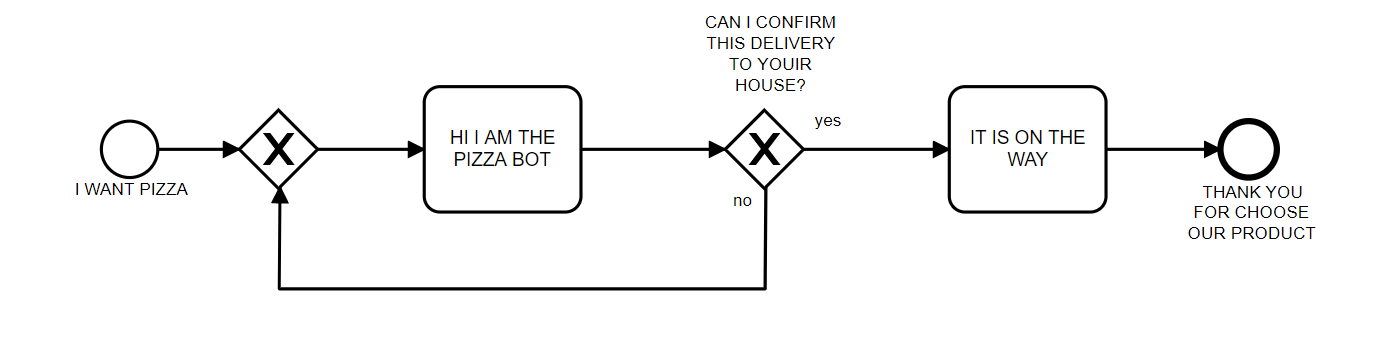
\includegraphics[width=1\linewidth]{./fig/fluxo.png}
	\label{fig:fluxo}
\end{figure}

Um outro tipo de fluxo para um chatbot que vende roupas está representada na Figura~\ref{fig:representacaodeumaarvore}.

\begin{figure}
\caption{Representação de uma árvore de decisão para comprar roupas online}
\vspace{0.5cm}
    \centering
   	\vspace*{0,2cm}
    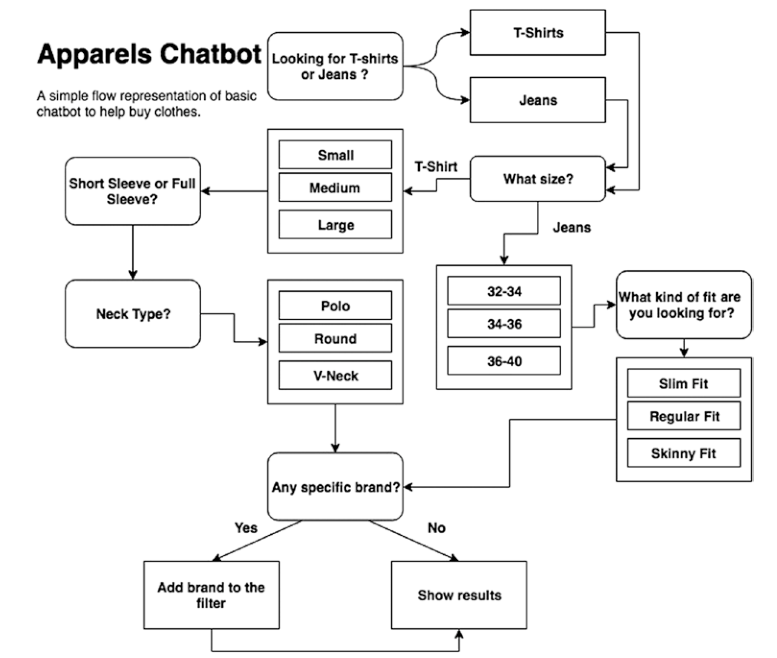
\includegraphics[width=0.9\textwidth]{./fig/image14.png}
    \label{fig:representacaodeumaarvore}
	{
	
	Retirado de \cite{Raj2019}.}
\end{figure}

\section{Histórico}

% \marginnote{AIML}
Um marco significativo na evolução dos chatbots depois do ELIZA foi o ALICE, que introduziu a Artificial Intelligence Markup Language (AIML), uma linguagem de marcação baseada em XML \cite{Wallace2000}. 
A AIML estabeleceu um paradigma para a construção de agentes conversacionais ao empregar algoritmos de correspondência de padrões. 
Essa abordagem utiliza modelos pré-definidos para mapear as entradas do usuário a respostas correspondentes, permitindo a definição modular de blocos de conhecimento \cite{Wallace2000}.

No contexto brasileiro, um dos primeiros chatbots documentados capaz de interagir em português, inspirado no modelo ELIZA, foi o Cybele \cite{primo2001chatterbot}. Posteriormente, foi desenvolvido o Elecktra, também em língua portuguesa, com aplicação voltada para a educação a distância \cite{Leonhardt2003}. 
Em um exemplo mais recente de aplicação governamental, no ano de 2019, o processo de inscrição para o Exame Nacional do Ensino Médio (ENEM) foi disponibilizado por meio de uma interface conversacional baseada em chatbot (Figura~\ref{fig:enem}).

\begin{figure}
	\centering
	\caption{Interface de chatbot para inscrição no ENEM 2019.}
	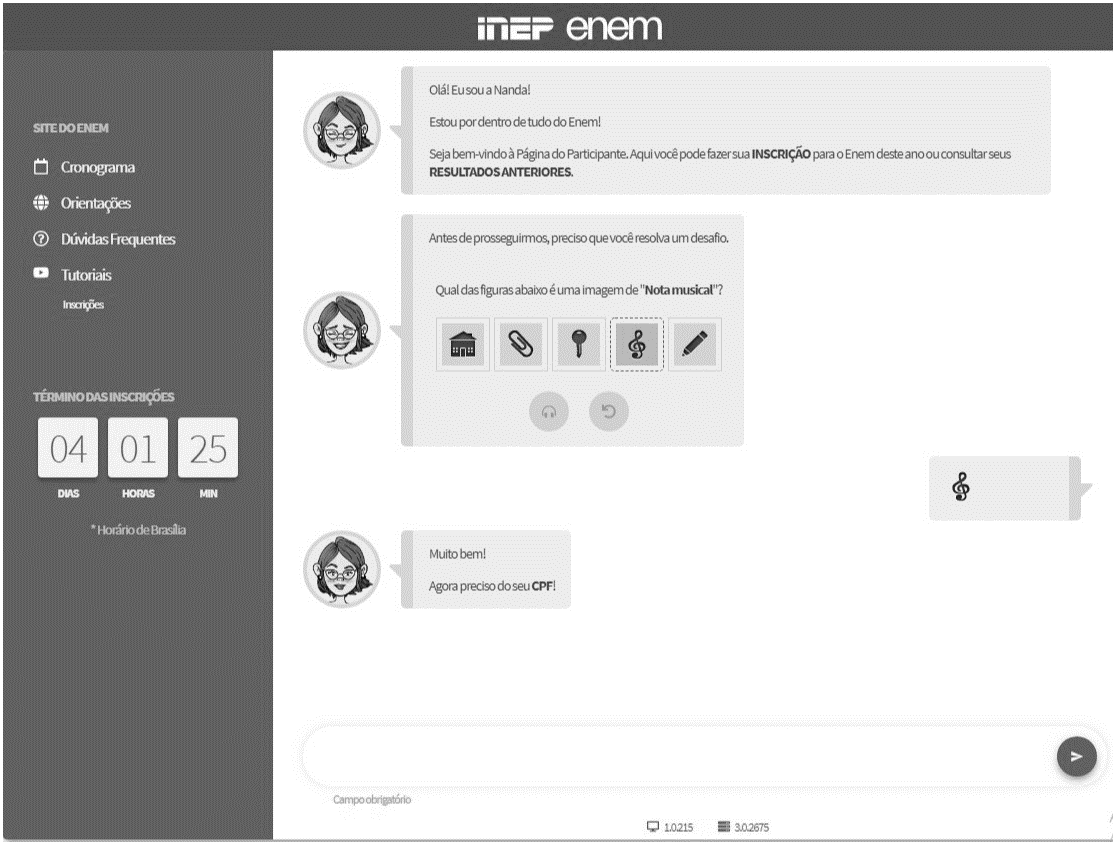
\includegraphics[width=0.5\linewidth]{./fig/enem.png}
	\label{fig:enem}
	{\footnotesize 
	
	Fonte: Captura de tela realizada por Giseldo Neo.}
\end{figure}

O desenvolvimento de chatbots avançados tem atraído investimentos de grandes corporações. Notavelmente, a IBM desenvolveu um sistema de resposta a perguntas em domínio aberto utilizando sua plataforma Watson \cite{Ferrucci2012}. Esse tipo de tarefa representa um desafio computacional e de inteligência artificial (IA) considerável. Em 2011, o sistema baseado em Watson demonstrou sua capacidade ao competir e vencer competidores humanos no programa de perguntas e respostas JEOPARDY! \cite{Ferrucci2012}.

Diversos outros chatbots foram desenvolvidos para atender a demandas específicas em variados domínios. Exemplos incluem: BUTI, um companheiro virtual com computação afetiva para auxiliar na manutenção da saúde cardiovascular \cite{Junior2008}; EduBot, um agente conversacional projetado para a criação e desenvolvimento de ontologias com lógica de descrição \cite{Lima2017}; PMKLE, um ambiente inteligente de aprendizado focado na educação em gerenciamento de projetos \cite{Torreao2005}; RENAN, um sistema de diálogo inteligente fundamentado em lógica de descrição \cite{AZEVEDO2015}; e MOrFEu, voltado para a mediação de atividades cooperativas em ambientes inteligentes na Web \cite{Bada2012}.

Entre os chatbots baseado em LLMs de destaque atualmente estão o Qwen, desenvolvido pela Alibaba, que se destaca por sua eficiência e suporte multilíngue; o DeepSeek, de código aberto voltado para pesquisa e aplicações empresariais com foco em precisão e escalabilidade; o Maritaca, modelo brasileiro de otimizado para o português; o Gemini, da Google, que integra capacidades multimodais e forte desempenho em tarefas diversas; o Mixtral, da Mistral AI, que utiliza arquitetura de mistura de especialistas para maior eficiência; o Llama, da Meta, reconhecido por ser código aberto e ampla adoção na comunidade; o Claude, da Anthropic, projetado com ênfase em segurança, alinhamento ético que vem ganhando adeptos para tarefas e codificação; e o Nemotron, da NVIDIA, que oferece modelos de linguagem otimizados para execução em GPUs e aplicações empresariais de alto desempenho. 

\section{Abordagens}

% \marginnote{Outras técnicas}
Desde o pioneirismo do ELIZA, múltiplas abordagens e técnicas foram exploradas para o desenvolvimento de chatbots. 
Entre as mais relevantes, destacam-se: AIML com correspondência de padrões (pattern matching), análise sintática (Parsing), modelos de cadeia de Markov (Markov Chain Models), uso de ontologias, redes neurais recorrentes (RNNs), redes de memória de longo prazo (LSTMs), modelos neurais sequência-a-sequência (Sequence-to-Sequence), aprendizado adversarial para geração de diálogo, além de abordagens baseadas em recuperação (Retrieval-Based) e generativas (Generative-Based) \cite{Borah2019, Ramesh2019, Shaikh2016, Abdul-Kader2015, Li2018}, entre outras.

\begin{itemize}
	\item ELIZA: o primeiro chatbot, que utilizava correspondência de padrões simples para simular um psicoterapeuta. O ELIZA foi um marco na história dos chatbots e influenciou o desenvolvimento de sistemas conversacionais subsequentes \cite{Weizenbaum1996}.
	\item AIML: Artificial Intelligence Markup Language, uma linguagem de marcação baseada em XML \cite{Wallace2000}. Essa linguagem permite a definição de regras de correspondência de padrões (pattern matching) para mapear entradas do usuário a respostas predefinidas. O AIML é amplamente utilizado na construção de chatbots, permitindo a criação de diálogos complexos e interativos.
	\item Modelos de Markov: introdução de técnicas de aprendizado de máquina, como os modelos ocultos de Markov (HMMs) , que utilizam cadeias de Markov para modelar sequências de palavras e prever a próxima palavra em uma sequência. % \cite{Bengio2003}
	\item Word2Vec: técnica de representação de palavras em vetores densos, permitindo capturar semântica e relações entre palavras. Essa técnica é frequentemente utilizada em chatbots para melhorar a compreensão do contexto e a geração de respostas. % \cite{Mikolov2013}
	\item TransformersBERT: arquitetura de rede neural baseada em atenção, que revolucionou o processamento de linguagem natural (NLP) \cite{Vaswani2017}. Modelos como BERT  e GPT  são exemplos de arquiteturas baseadas em Transformers que têm sido amplamente utilizadas em chatbots modernos. % \cite{Devlin2018} % \cite{Radford2019}
	\item GPT: modelos de linguagem generativa, como o GPT-3 , que utilizam redes neurais profundas para gerar texto coerente e relevante em resposta a entradas do usuário. Esses modelos são treinados em grandes quantidades de dados e podem ser adaptados para tarefas específicas, como atendimento ao cliente ou suporte técnico. % \cite{Brown2020}
\end{itemize}

Além disso, diversos frameworks têm sido desenvolvidos para facilitar a criação desses agentes complexos, como CrewAI e bibliotecas associadas a plataformas como Hugging Face (e.g., Transformers Agents), que fornecem abstrações e ferramentas em Python para orquestrar múltiplos componentes e o uso de ferramentas externas.

\section{Problemática}	

Apesar do progresso recente de chatbots, como o ChatGPT, o mecanismo fundamental da inteligência em nível humano, frequentemente refletido na comunicação, ainda não está totalmente esclarecido \cite{Shum2018}. 
Para avançar na solução desses desafios, serão necessários progressos em diversas áreas da IA cognitiva, tais como: modelagem empática de conversas, modelagem de conhecimento e memória, inteligência de máquina interpretável e controlável, e calibração de recompensas emocionais \cite{Shum2018}.

Uma das dificuldades na construção de chatbots do tipo orientado a tarefas reside em gerenciar a complexidade das estruturas condicionais ("se-então") que definem o fluxo do diálogo \cite{Raj2019}. Quanto maior o número de decisões a serem tomadas, mais numerosas e intrincadas tendem a ser essas estruturas condicionais. Contudo, elas são essenciais para codificar fluxos de conversação complexos. 
Se a tarefa que o chatbot visa simular é inerentemente complexa e envolve múltiplas condições, o código precisará refletir essa complexidade. 
Para facilitar a visualização desses fluxos, uma solução eficaz é a utilização de fluxogramas.  % TODO Citar Giseldo Neo
Embora simples de criar e entender, os fluxogramas constituem uma poderosa ferramenta de representação para este problema.

Os chatbots baseados em AIML apresentam desvantagens específicas. Por exemplo, o conhecimento é representado como instâncias de arquivos AIML. 
Se esse conhecimento for criado com base em dados coletados da Internet, ele não será atualizado automaticamente, exigindo atualizações periódicas manuais \cite{Madhumitha2015}. 
No entanto, já existem abordagens para mitigar essa limitação, permitindo carregar conteúdo AIML a partir de fontes como arquivos XML \cite{Macedo2014}, um corpus textual \cite{DeGasperis2013} ou dados do Twitter \cite{Yamaguchi2018}.

Outra desvantagem do AIML, a exemplo do Eliza, reside na relativa complexidade de seus padrões de correspondência (patterns). Além disso, a manutenção do sistema pode ser árdua, pois, embora a inserção de conteúdo (categorias) seja conceitualmente simples, grandes volumes de informação frequentemente precisam ser adicionados manualmente \cite{Madhumitha2015}.

Especificamente no caso do AIML, a construção e a visualização de fluxos de diálogo complexos enfrentam dificuldades adicionais. Devido ao seu formato baseado em texto, muitas vezes é difícil perceber claramente como as diferentes categorias (unidades de conhecimento e resposta) se interligam para formar a estrutura da conversação.

% TODO : Rasa PRO

\section{Exercícios}

\begin{enumerate}

\item \textbf{Qual é o objetivo principal de um chatbot?} 
\begin{enumerate}[label=\alph*)]
\item Substituir completamente os seres humanos no atendimento ao cliente. 
\item Simular uma conversa humana para resolver problemas ou fornecer informações. 
\item Gerar textos literários complexos. 
\item Armazenar grandes quantidades de dados em tempo real. 
\end{enumerate}
%B

\item \textbf{Qual das seguintes opções descreve corretamente um benefício dos chatbots?} 
\begin{enumerate}[label=\alph*)]
\item Eles nunca precisam ser atualizados. 
\item Eles podem operar 24 horas por dia, 7 dias por semana, sem intervenção humana. 
\item Eles sempre tomam decisões melhores do que humanos. 
\item Eles substituem completamente a necessidade de suporte técnico. 
\end{enumerate}
%B

\item \textbf{Qual das opções a seguir é uma técnica comum usada por chatbots para entender o que o usuário está perguntando?} 
\begin{enumerate}[label=\alph*)]
\item Mineração de Dados 
\item Tokenização 
\item Compressão de Dados 
\item Balanceamento de Carga 
\end{enumerate}
%B

\item \textbf{Qual é o papel dos embeddings de palavras em chatbots?} 
\begin{enumerate}[label=\alph*)]
\item Converter palavras em vetores numéricos que capturam o significado semântico. 
\item Armazenar grandes quantidades de dados de conversação. 
\item Executar algoritmos de compressão de texto. 
\item Facilitar a tradução de texto entre diferentes idiomas. 
\end{enumerate}
%A

\item \textbf{Qual é a principal limitação dos chatbots baseados em regras?}
\begin{enumerate}[label=\alph*)]
\item Eles não conseguem operar em tempo real. 
\item Eles exigem grandes quantidades de dados para funcionar. 
\item Eles só podem responder a consultas específicas para as quais foram \item programados. 
\item Eles são incapazes de realizar tarefas repetitivas. 
\end{enumerate}
% C

\end{enumerate}

%%%%%%%%%%%%%%%%
%%%%CAPITULO%%%%
%%%%%%%%%%%%%%%%

\chapter{Eliza}

\section{Introdução}

o ELIZA foi um dos primeiros programas de processamento de linguagem natural e foi apresentado em 1966 por Joseph Weizenbaum no MIT \cite{Weizenbaum1996}.

% \marginnote{SCRIPT}
O conjunto de padrões e respostas predefinidas constitui o que Weizenbaum chamou de “roteiro” (ou script) de conversa. O mecanismo do ELIZA separa o motor de processamento, sendo o algoritmo de busca de palavras-chave e aplicação de regras, dos dados do script em si. 
Isso significa que ELIZA podia em teoria simular diferentes personalidades ou tópicos apenas carregando um script diferente, sem alterar o código do programa (veja na Figura~\ref{fig:elizaeditor}). Também foi codificado um editor de texto para as alterações do próprio Script.

\begin{figure}[!htbp]
	\centering	
	\caption{ELIZA: separação entre o código fonte, o script e o editor de texto.}
	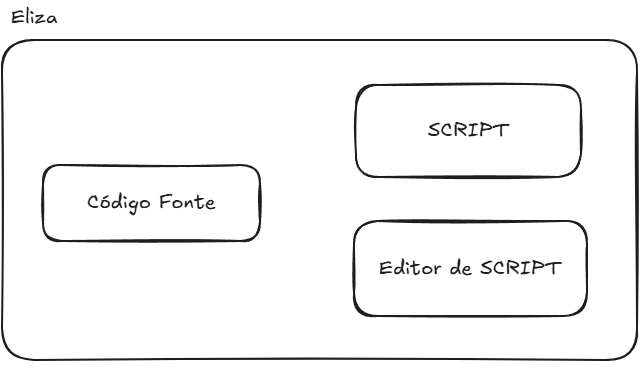
\includegraphics[width=0.9\linewidth]{./fig/eliza.png}
	\label{fig:elizaeditor}
\end{figure}

% \marginnote{SCRIPT DOCTOR}
Um destes roteiros, o script DOCTOR, deixou o ELIZA famoso. 
Com este script carregado, o ELIZA simulava precariamente um psicoterapeuta (do estilo Rogeriano), refletindo as palavras do usuário de volta em forma de pergunta. 
% A primeira linha do script é a introdução do chatbot, a primeira palavra que ele escrever para o usuário. 
% START é um comando técnico do script, serve para indicar que a seguir virão as regras. 


Veja na lista~\ref{lst:script} uma parte do conteúdo do DOCTOR. A primeira linha REMEMBER 5 estabelece que a prioridade da palavra REMEMBER é 5, caso o usuário entre com uma frase com a palavra REMEMBER, o ELIZA irá responder com uma das perguntas definidas nos parênteses, dentro do nível da palavra REMENBER. 
A segunda lista dentro do REMEMBER são as regras de transformação de frases (decomposition rule e reassembly rule) associadas à palavra-chave REMEMBER. O mesmo se repete para a palavra IF que tem um peso difernte de REMEMBER.

\begin{lstlisting}[caption=Roteiro Script Doctor, label=lst:script]
(REMEMBER 5 
	(
		(0 YOU REMEMBER 0) 
		(DO YOU OFTEN THINK OF 4) 
		(DOES THINKING OF ~ BRING ANYTHING ELSE TO MINO) 
		(WHAT ELSE OO YOU REMEMBER)
		(WHY DO YOU REMEMBER 4 JUST NOW) 
		(WHAT IN THE PRESENT SITUATION REMINDS YOU OF 4) 
		(WHAT IS THE CONNECTION BETWEEN ME AND 4)
	) 
	(
		(0 DO I REMEMBER 0) 
		(DID YOU THINK I WOULD FORGET 5) 
		(WHY DO YOU THINK I SHOULD RECALL 5 NOW) 
		(WHAT ABOUT 5) 
		(=WHAT) 
		(YOU MENTIONED S)
	) 
) 

(IF 3 
	(
		(0 IF 0) 
		(DO YOU THINK ITS LIKELY THAT 3) 
		(DO YOU WISH THAT 3) 
		(WHAT DO YOU THINK ABOUT 3) 
		(REALLY, 2 3)
	)
.... continua
	
\end{lstlisting}

Na lista~\ref{lst:exemplodialogoeliza} é apresentado um exemplo de diálogo (retirado do artigo original) entre um usuário humano e ELIZA, mostrando as respostas em letras maiúsculas. 
Nesse exemplo, o usuário faz afirmações pessoais (“Men are all alike.”, “Well, my boyfriend made me come here.”) e ELIZA responde com perguntas ou reformulações (“IN WHAT WAY”, “YOUR BOYFRIEND MADE YOU COME HERE?”), reutilizando termos do próprio usuário. Esse estilo reflexivo encoraja o usuário a continuar falando sem fornecer respostas diretas.

\begin{lstlisting}[language=Clean, caption=Exemplo de diálogo do ELIZA, label=lst:exemplodialogoeliza]
Men are all alike. 
IN WHAT WAY 
They're always bugging us about something or other. 
CAN YOU THINK OF A SPECIFIC EXAMPLE 
Well, my boyfriend made me come here. 
YOUR BOYFRIEND MADE YOU COME HERE 
He says I'm depressed much of the time. 
I AM SORRY TO HEAR YOU ARE DEPRESSED 
It's true. I am unhappy. 
DO YOU THINK COMING HERE WILL HELP YOU NOT TO BE UNHAPPY 
I need some help, that much seems certain. 
WHAT WOULD IT MEAN TO YOU IF YOU GOT SOME HELP 
Perhaps I could learn to get along with my mother. 
TELL ME MORE ABOUT YOUR FAMILY 
My mother takes care of me. 
WHO ELSE IN YOUR FAMILY TAKES CARE OF YOU 
My father. 
YOUR FATHER 
You are like my father in some ways. 
WHAT RESEMBLANCE DO YOU SEE 
You are not very aggressive but I think you don't want me to 
notice that. 
WHAT MAKES YOU THINK I AM NOT VERY AGGRESSIVE 
You don't argue with me. 
WHY DO YOU THINK I DON'T ARGUE WITH YOU 
You are afraid of me. 
DOES IT PLEASE YOU TO BELIEVE I AM AFRAID OF YOU 
My father is afraid of everybody. 
WHAT ELSE COMES TO MIND WHEN YOU THINK OF YOUR FATHER 
Bullies. 
DOES THAT HAVE ANYTHING TO DO WITH THE FACT THAT YOUR BOYFRIEND MADE YOU COME HERE 
\end{lstlisting}
	

% Um detalhamento do algoritmo do ELIZA está no Algoritmo 1.

% Algoritmo 1 - Algoritmo Eliza

% Fonte: Buscar a Fonte do Algoritmo Adaptado por Giseldo Neo

\section{Processamento de Entradas e Palavras-Chave}

% \marginnote{Pattern Matching}
O funcionamento do ELIZA baseia-se em correspondência de padrões por palavras-chave. Técnica também chamado casamento de padrão, em inglês \textit{pattner matching} seu paradigma também se encaixa na técnica baseado em regras (ou \textit{rule-based}). 
A cada turno, o texto de entrada do usuário é analisado em busca de palavras-chave predefinidas. 
O ELIZA fazia uma varredura da sentença da esquerda para a direita, identificando se alguma palavra correspondia a uma palavra\-chave do script. 
Caso encontrasse, ELIZA selecionava a palavra-chave mais “importante” (havia um peso de prioridade associado a cada palavra-chave) e ignorava o restante da entrada.

Por exemplo, o script DOCTOR, definia palavras-chave como “ALIKE” ou “SAME” com alta prioridade; assim, na frase “Men are all alike.” o programa detectava a palavra “ALIKE” e disparava uma resposta associada a ela (no caso: “In what way?”). 
Se múltiplas palavras-chave aparecessem, ELIZA escolhia aquela de maior peso para formular a resposta.

Primeiro o texto de entrada digitado pelo usuário era separado em palavras, em um técnica que hoje chamamos de tokenização de palavras. A palavra-chave era identificada, comparando-a sequencialmente até o fim das palavras existentes, ou até ser encontrado uma pontuação. Caso fosse encontrado uma pontuação (ponto final ou vírgula), o texto após a pontuação era ignorado se já tivesse sido identificado uma palavra-chave. Assim cada processamento da resposta foca em apenas uma única afirmação (ou frase) do usuário. Se várias palavras-chave fossem encontradas antes da pontuação, a de maior peso era selecionada.

Por exemplo, o usuário entra com o texto: “I am sick. but, today is raining”. Se houvesse uma palavra-chave no script rankeando a palavra “SICK" com alta prioridade, a entrada processada seria somente “I am sick”, o restante depois da pontuação (neste caso, o ponto) seria gnorado pelo programa.

Se nenhuma palavra-chave fosse encontrada na entrada, ELIZA recorria a frases genéricas programadas, chamadas de respostas vazias ou sem conteúdo. Nesses casos, o chatbot emitia mensagens do tipo “I see.” ou “Please, go on.” . Esse mecanismo evitava silêncio quando o usuário dizia algo fora do escopo do script.

Além disso, a implementação original incluía uma estrutura de memória: algumas declarações recentes do usuário eram armazenadas e, se uma entrada subsequente não contivesse novas keywords, ELIZA poderia recuperar um tópico anterior e introduzi-lo na conversa.
Por exemplo, se o usuário mencionasse família em um momento e depois fizesse uma afirmação vaga, o programa poderia responder retomando o assunto da família (“DOES THAT HAVE ANYTHING TO DO WITH YOUR FAMILY?”).
Essa estratégia dava uma pseudo-continuidade ao diálogo, simulando que o sistema “lembrava” de informações fornecidas anteriormente.

\section{Regras de Transformação de Frases}

Encontrada a palavra-chave, ELIZA aplicava uma regra de transformação associada a ela para gerar a resposta. As regras são definidas em pares: um padrão de análise (decomposition rule) e um modelo de reconstrução de frase (reassembly rule).

Primeiro, a frase do usuário é decomposta conforme um padrão que identifica a contexto mínimo em torno da palavra-chave. Essa decomposição frequentemente envolve separar a frase em partes e reconhecer pronomes ou estruturas gramaticais relevantes. Por exemplo, considere a entrada “You are very helpful.”. Uma regra de decomposição pode identificar a estrutura “You are X” — onde “X” representa o restante da frase — e extrair o complemento “very helpful” como um componente separado.

Em seguida, a regra de reassembly correspondente é aplicada, remontando uma sentença de resposta em que “X” é inserido em um template pré-definido. No exemplo dado, o template de resposta poderia ser “What makes you think I am X?”; ao inserir X = “very helpful”, gera-se “What makes you think I am very helpful?”. Observe que há uma inversão de pessoa: o pronome “you” do usuário foi trocado por “I” na resposta do bot.

De fato, uma parte importante das transformações do ELIZA envolve substituir pronomes (eu/você, meu/seu) para que a resposta faça sentido como uma frase do ponto de vista do computador falando com o usuário. Esse algoritmo de substituição é relativamente simples (por exemplo, “meu” → “seu”, “eu” → “você”, etc.), mas essencial para dar a impressão de entendimento gramatical.

\section{Implementação Original e Variações Modernas}

A implementação original de ELIZA foi feita em uma linguagem chamada MAD-SLIP (um dialecto de Lisp) rodando em um mainframe IBM 7094 no sistema CTSS do MIT. O código fonte do programa principal continha o mecanismo de correspondência, enquanto as regras de conversação (script DOCTOR) eram fornecidas separadamente em formato de listas associativas, similar a uma lista em Lisp. Infelizmente, Weizenbaum não publicou o código completo no artigo de 1966 (o que era comum na época), mas décadas depois o código em MAD-SLIP foi recuperado nos arquivos do MIT, comprovando os detalhes de implementação \cite{Lane2025}. De qualquer forma, a arquitetura descrita no artigo influenciou inúmeras reimplementações acadêmicas e didáticas nos anos seguintes.

Diversos entusiastas e pesquisadores reescreveram ELIZA em outras linguagens de programação, dada a simplicidade relativa de seu algoritmo. Ao longo dos anos surgiram versões em Lisp, PL/I, BASIC, Pascal, Prolog, Java, Python, OZ, JavaScript, entre muitas outras. Cada versão normalmente incluía o mesmo conjunto de regras do script terapeuta ou pequenas variações.

As ideias de ELIZA também inspiraram chatbots mais avançados. Poucos anos depois, em 1972, surgiu PARRY, escrito pelo psiquiatra Kenneth Colby, que simulava um paciente paranoico. PARRY tinha um modelo interno de estado emocional e atitudes, mas na camada de linguagem ainda usava muitas respostas baseadas em regras, chegando a “conversar” com o próprio ELIZA em experimentos da época.

Em 1995, Richard Wallace desenvolveu o chatbot ALICE (Artificial Linguistic Internet Computer Entity), que levava o paradigma de ELIZA a uma escala muito maior. ALICE utilizava um formato XML chamado AIML (Artificial Intelligence Markup Language) para definir milhares de categorias de padrões e respostas. Com mais de 16.000 templates mapeando entradas para saídas \cite{Wallace2000}, ALICE conseguia manter diálogos bem mais naturais e abrangentes que o ELIZA original, embora o princípio básico de correspondência de padrões permanecesse. Esse avanço rendeu a ALICE três vitórias no Prêmio Loebner (competição de chatbots) no início dos anos 2000 \cite{Wallace2000}.

Outras variações e sucessores notáveis incluem Jabberwacky (1988) – que já aprendia novas frases – e uma profusão de assistentes virtuais e bots de domínio específico nas décadas seguintes \cite{Wallace2000}. Em suma, o legado de ELIZA perdurou por meio de inúmeros chatbots baseados em regras, até a transição para abordagens estatísticas e de aprendizado de máquina no final do século XX.

\section{Comparação com Modelos de Linguagem Modernos}

A técnica de ELIZA, baseada em palavras-chave com respostas predefinidas, contrasta fortemente com os métodos de Large Language Models (LLMs) atuais, como o GPT-4, que utilizam redes neurais de milhões (ou trilhões) de parâmetros e mecanismos de atenção.

\subsection{Mecanismo de Pesos: Palavras-Chave vs. Atenção Neural}

No ELIZA, a “importância” de uma palavra era determinada manualmente pelo programador através de pesos ou rankings atribuídos a certas palavras-chave no script. Ou seja, o programa não aprendia quais termos focar – ele seguia uma lista fixa de gatilhos. Por exemplo, termos como “sempre” ou “igual” tinham prioridade alta no script DOCTOR para garantir respostas apropriadas.

Em contraste, modelos modernos como o GPT não possuem uma lista fixa de palavras importantes; em vez disso, eles utilizam o mecanismo de self-attention para calcular dinamicamente pesos entre todas as palavras da entrada conforme o contexto \cite{Vaswani2017}.

Na arquitetura Transformer, cada palavra (token) de entrada gera consultas e chaves que interagem com todas as outras, permitindo ao modelo atribuir pesos maiores às palavras mais relevantes daquela frase ou parágrafo \cite{Vaswani2017}. Em outras palavras, o modelo aprende sozinho quais termos ou sequências devem receber mais atenção para produzir a próxima palavra na resposta. Esse mecanismo de atenção captura dependências de longo alcance e nuances contextuais que um sistema de palavras-chave fixas como o ELIZA não consegue representar.

Além disso, o “vocabulário” efetivo de um LLM é imenso – um moddelo GPT pode ser treinado com trilhões de palavras e ter ajustado seus parâmetros para modelar estatisticamente a linguagem humana \cite{Vaswani2017}. Como resultado, pode-se dizer metaforicamente que os LLMs têm uma lista de “palavras-chave” milhões de vezes maior (na prática, distribuída em vetores contínuos) e um método bem mais sofisticado de calcular respostas do que o ELIZA.

Enquanto ELIZA dependia de coincidências exatas de termos para disparar regras, modelos como GPT avaliam similaridades semânticas e contexto histórico graças às representações densas (embeddings) aprendidas durante o treinamento de rede neural.

\subsection{Contextualização e Geração de Linguagem}

Devido à sua abordagem baseada em regras locais, o ELIZA tinha capacidade de contextualização muito limitada. Cada input do usuário era tratado quase isoladamente: o programa não construía uma representação acumulada da conversa, além de artifícios simples como repetir algo mencionado (a estrutura de memória) ou usar pronomes para manter a ilusão de continuidade. Se o usuário mudasse de tópico abruptamente, o ELIZA não “perceberia” – ele apenas buscaria a próxima palavra-chave disponível ou recorreria a frases genéricas.

Em contraste, modelos de linguagem modernos levam em conta um longo histórico de diálogo. Chatbots que usam GPT podem manter um contexto centenas ou milhares de tokens (palavras ou fragmentos) em sua janela de atenção, o que significa que eles conseguem referenciar informações mencionadas vários parágrafos atrás e integrá-las na resposta corrente. O mecanismo de self-attention, em particular, permite que o modelo incorpore relações contextuais complexas: cada palavra gerada pode considerar influências de palavras distantes no texto de entrada \cite{Vaswani2017}.

Por exemplo, ao conversar com um LLM, se você mencionar no início da conversa que tem um irmão chamado Alex e depois perguntar “ele pode me ajudar com o problema?”, o modelo entenderá que “ele” se refere ao Alex mencionado anteriormente (desde que dentro da janela de contexto). Já o ELIZA original não teria como fazer essa ligação, a menos que houvesse uma regra explícita para “ele” e algum armazenamento específico do nome – algo impraticável de antecipar via regras fixas para todos os casos.

Outra diferença está na geração de linguagem. O ELIZA não gera texto original no sentido pleno: suas respostas são em grande parte frases prontas (ou templates fixos) embaralhadas com partes da fala do usuário. Assim, seu vocabulário e estilo são limitados pelo script escrito manualmente. Modelos GPT, por sua vez, geram respostas novas combinando probabilisticamente o conhecimento adquirido de um extenso corpus. Eles não se restringem a repetir trechos da entrada, podendo elaborar explicações, fazer analogias, criar perguntas inéditas – tudo coerente com os exemplos linguísticos em sua base de treinamento. Enquanto ELIZA tendia a responder com perguntas genéricas ou devolvendo as palavras do usuário, os LLMs podem produzir respostas informativas e detalhadas sobre o assunto (pois “aprenderam” uma ampla gama de tópicos durante o treinamento). Por exemplo, se perguntarmos algo factual ou complexo, o ELIZA falharia por não ter nenhuma regra a respeito, provavelmente dando uma resposta vazia. Já um modelo como GPT-4 tentará formular uma resposta baseada em padrões linguísticos aprendidos e em conhecimento implícito dos dados, muitas vezes fornecendo detalhes relevantes.

Em termos de fluência e variedade, os modelos modernos superam o ELIZA amplamente. O ELIZA frequentemente se repetia ou caía em loops verbais quando confrontado com inputs fora do roteiro – um limite claro de sistemas por regras estáticas. Os LLMs produzem linguagem muito mais natural e adaptável, a ponto de muitas vezes enganarem os usuários sobre estarem conversando com uma máquina (um efeito buscado desde o Teste de Turing). Ironicamente, ELIZA nos anos 60 já provocou um precursor desse fenômeno – o chamado Efeito ELIZA, em que pessoas atribuem compreensão ou sentimentos a respostas de computador que, na verdade, são superficiais. Hoje, em chatbots GPT, esse efeito se intensifica pela qualidade das respostas, mas a distinção fundamental permanece: ELIZA seguia scripts sem compreender, enquanto LLMs inferem padrões e significados de forma estatística, sem entendimento consciente, mas atingindo resultados que simulam compreensão de maneira muito mais convincente. 

Em resumo, os avanços de arquitetura (especialmente o mecanismo de atenção) ampliaram drasticamente a capacidade de contextualização e geração dos chatbots modernos, marcando uma evolução significativa desde o mecanismo simples porém pioneiro de ELIZA.

\section{Implementação de um Chatbot Simples em Python}

Abaixo está um exemplo básico de implementação de um chatbot inspirado em Eliza utilizando Python:

\begin{lstlisting}[language=Python, caption=Exemplo simples do Eliza,label=lst:eliza_chatbot]
import re

# Regras de substituição simples
reflections = {
	"eu": "você",
	"meu": "seu",
	"você": "eu",
	"me": "te",
}

def eliza_response(user_input):
	for word, replacement in reflections.items():
	user_input = re.sub(r'\b{}\b'.format(word), replacement, user_input)
	return user_input

# Exemplo de uso
while True:
	user_input = input("Você: ")
	if user_input.lower() in ["sair", "tchau"]:
	break
	response = eliza_response(user_input)
	print("Eliza: ", response)
\end{lstlisting}

\section{Eliza em Python}

Apresenta-se, nesta seção, uma implementação simplificada em Python de um chatbot inspirado no paradigma ELIZA. 
Esta implementação demonstra a utilização de expressões regulares para a identificação de padrões textuais (palavras-chave) na entrada fornecida pelo usuário e a subsequente geração de respostas, fundamentada em regras de transformação predefinidas manualmente.

\vspace{\baselineskip}
\href{https://colab.research.google.com/github/giseldo/chatbotbook/blob/main/notebook/eliza.ipynb}{
  
\includegraphics{./fig/colab-badge.png}
}

\begin{lstlisting}[language=Python, caption=Chatbot Eliza em Python]
import re  
import random  

regras = [
    (re.compile(r'\b(hello|hi|hey)\b', re.IGNORECASE),
     ["Hello. How do you do. Please tell me your problem."]),

    (re.compile(r'\b(I am|I\'?m) (.+)', re.IGNORECASE),
     ["How long have you been {1}?",   
      "Why do you think you are {1}?"]),

    (re.compile(r'\bI need (.+)', re.IGNORECASE),
     ["Why do you need {1}?",
      "Would it really help you to get {1}?"]),

    (re.compile(r'\bI can\'?t (.+)', re.IGNORECASE),
     ["What makes you think you can't {1}?",
      "Have you tried {1}?"]),

    (re.compile(r'\bmy (mother|father|mom|dad)\b', re.IGNORECASE),
     ["Tell me more about your family.",
      "How do you feel about your parents?"]),

    (re.compile(r'\b(sorry)\b', re.IGNORECASE),
     ["Please don't apologize."]),

    (re.compile(r'\b(maybe|perhaps)\b', re.IGNORECASE),
     ["You don't seem certain."]),

    (re.compile(r'\bbecause\b', re.IGNORECASE),
     ["Is that the real reason?"]),

    (re.compile(r'\b(are you|do you) (.+)\?$', re.IGNORECASE),
     ["Why do you ask that?"]),

    (re.compile(r'\bcomputer\b', re.IGNORECASE),
     ["Do computers worry you?"]),
]

respostas_padrao = [
    "I see.",  
    "Please tell me more.",  
    "Can you elaborate on that?"  
]

def response(entrada_usuario):
    for padrao, respostas in regras:
        match = padrao.search(entrada_usuario)  
        if match:
            resposta = random.choice(respostas)
            if match.groups():
                resposta = resposta.format(*match.groups())
            return resposta
    return random.choice(respostas_padrao)
\end{lstlisting}

\begin{lstlisting}[language=Python, caption=Exemplo de uso do chatbot ELIZA]
print("User: Hello.")
print("Bot: " + response("Hello."))

print("User: I am feeling sad.")
print("Bot: " + response("I am feeling sad."))

print("Maybe I was not good enough.")
print("Bot: " + response("Maybe I was not good enough."))

print("My mother tried to help.")
print("Bot: " + response("My mother tried to help."))
\end{lstlisting}

Na implementação, são definidos múltiplos padrões de expressões regulares que correspondem a palavras-chave ou estruturas frasais de interesse (e.g., saudações, construções como ``I am'' ou ``I need'', referências a termos familiares). A função \texttt{response}, ao receber uma string de entrada, itera sequencialmente sobre essas regras. Para cada regra, utiliza-se o método \texttt{padrao.search(entrada)} para verificar a ocorrência do padrão correspondente na sentença do usuário.

Quando uma correspondência (match) é encontrada, uma resposta associada à regra é selecionada. É relevante notar que diversas respostas predefinidas contêm marcadores (placeholders), como \texttt{\{1\}}. Estes marcadores são dinamicamente substituídos pelo conteúdo dos grupos capturados pela expressão regular na entrada original do usuário. Por exemplo, se a entrada for \textit{``I am sad''} e esta corresponder a um padrão como \texttt{r"I am (.*)"}, o grupo capturado (\texttt{(.*)}) conterá a string \textit{``sad''}. Se a resposta associada for \textit{``Why do you think you are \{1\}?''}, o sistema a formatará como \textit{``Why do you think you are sad?''}, substituindo \texttt{\{1\}} pelo conteúdo do primeiro grupo capturado.

Na ausência de correspondência com qualquer regra específica, o sistema seleciona aleatoriamente uma resposta genérica a partir de um conjunto predefinido (denominado, por exemplo, \texttt{respostas\_padrao}), tal como \textit{``I see.''}.

% Usando  para um subtítulo menos proeminente, ou use \subsubsection se preferir
Exemplo de Interação:

\begin{lstlisting}
Usuário: Hello
Bot: Hello. How do you do. Please tell me your problem.

Usuário: I am feeling sad
Bot: Why do you think you are feeling sad?

Usuário: Because I lost my job
Bot: Is that the real reason?

Usuário: Maybe I was not good enough.
Bot: You don't seem certain.

Usuário: My mother tried to help.
Bot: Tell me more about your family.
\end{lstlisting}

Observa-se na interação que o chatbot inicialmente respondeu à saudação (\textit{``Hello...''}) com base na regra 1. Em seguida, a entrada \textit{``I am sad''} ativou a regra 2, resultando em uma resposta que incorpora o termo \textit{``sad''}. 
A interação prossegue com o sistema respondendo a entradas iniciadas por \textit{``Because...''} (regra 8) e \textit{``Maybe...''} (regra 7), entre outras. 
Cada resposta gerada foi determinada pela regra correspondente ativada e pelo conteúdo específico da sentença do usuário, mimetizando o comportamento baseado em padrões do sistema ELIZA original \cite{Abdul-Kader2015}.

%%%%%%%%%%%%%%%%
%%%%CAPITULO%%%%
%%%%%%%%%%%%%%%%

\chapter{Artificial Intelligence Markup
Language}

\section{Introdução}

O Artificial Intelligence Markup Language (AIML) é uma especificação baseada em XML, proposta por \cite{Wallace2009}, destinada à programação de agentes conversacionais, comumente denominados chatbots. 
A concepção da linguagem prioriza o minimalismo, característica que simplifica o processo de criação de bases de conhecimento por indivíduos sem experiência prévia em programação \cite{Wallace2009}. 
A arquitetura fundamental de um interpretador AIML genérico é ilustrada na Figura~\ref{fig:interpretador}.

\begin{figure}
    \centering
    \caption{Interpretador AIML arquitetura.}
    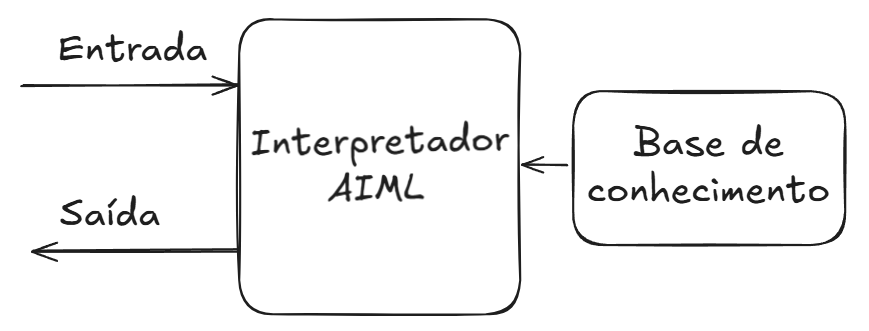
\includegraphics[width=0.8\textwidth]{./fig/aimlbase.png} 
    \label{fig:interpretador}
    \vspace{0.2cm} 
    {\footnotesize 
	
	Adaptado de \cite{Silva2007}}
\end{figure}

A técnica central empregada pelo AIML é a correspondência de padrões (\emph{pattern matching}). Este método é amplamente utilizado no desenvolvimento de chatbots, particularmente em sistemas orientados a perguntas e respostas \cite{Abdul-Kader2015}.
Uma das metas de projeto do AIML é possibilitar a fusão de bases de conhecimento de múltiplos chatbots especializados em domínios distintos.
Teoricamente, um interpretador poderia agregar essas bases, eliminando automaticamente categorias redundantes para formar um \emph{chatbot} mais abrangente \cite{Wallace2000}.

AIML é frequentemente associado aos chatbots de terceira geração \cite{Maria2010} e estima-se sua adoção em mais de 50.000 implementações em diversos idiomas. 
Extensões da linguagem foram propostas, como o iAIML, que introduziu novas \emph{tags} e incorporou o conceito de intenção com base nos princípios da Teoria da Análise da Conversação (TAC) \cite{Neves2005}. 
Adicionalmente, ferramentas baseadas na Web foram desenvolvidas para apoiar a construção de bases de conhecimento AIML \cite{Krassmann2017}. Um exemplo proeminente é o \emph{chatbot} ALICE, cuja implementação em AIML compreendia aproximadamente 16.000 categorias, cada uma potencialmente contendo múltiplas \emph{tags} XML aninhadas \cite{Wallace2000}. 
Uma representação visual desta estrutura de conhecimento é apresentada na Figura~\ref{fig:representacaovisual}.

\begin{figure}
    \centering
    \caption{Representação visual da base de conhecimento do chatbot ALICE.}
    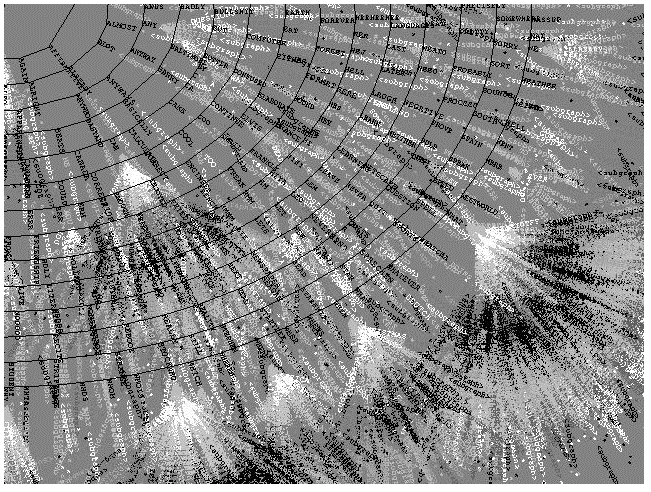
\includegraphics[width=0.7\textwidth]{./fig/image9.png} % Ajuste o caminho se necessário
    \label{fig:representacaovisual}
    \vspace{0.2cm} % Espaçamento opcional
    {\footnotesize 
	
	Retirado de \cite{Wallace2003}}
\end{figure}

\cite{Wallace2000} estabeleceu analogias entre o funcionamento de interpretadores AIML e a teoria do Raciocínio Baseado em Casos (RBC). Nessa perspectiva, as categorias AIML funcionam como "casos", onde o algoritmo identifica o padrão que melhor se alinha à entrada do usuário. 
Cada categoria estabelece um vínculo direto entre um padrão de estímulo e um modelo de resposta. Consequentemente, chatbots AIML inserem-se na tradição da robótica minimalista, reativa ou de estímulo-resposta \cite{Wallace2000}, conforme esquematizado na Figura~\ref{fig:teoriaestimulo}. 
Vale notar que a própria técnica de RBC já foi integrada a interpretadores AIML como um mecanismo para consultar fontes de dados externas e expandir a base de conhecimento do agente \cite{Kraus2008}.

\begin{figure}
    \centering
    \caption{Teoria estímulo-resposta aplicada no AIML}
    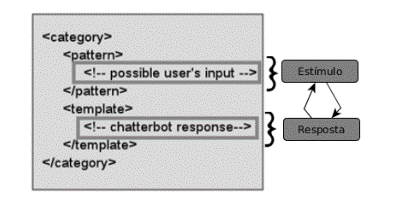
\includegraphics[width=0.7\textwidth]{./fig/image10.png} % 
    \label{fig:teoriaestimulo}
    \vspace{0.2cm}
    {\footnotesize 
	
	Retirado de \cite{Lima2017}}
\end{figure}

Os chatbots que utilizam AIML são classificados como sistemas "baseados em recuperação" (retrieval-based). 
Tais modelos operam a partir de um repositório de respostas predefinidas, selecionando a mais apropriada com base na entrada do usuário e no contexto conversacional, guiando assim o fluxo da interação. 
Esta abordagem é frequentemente empregada na construção de chatbots destinados a operar em domínios de conhecimento restritos \cite{Borah2019}.

A Figura~\ref{fig:exemplodeumabase} demonstra a estrutura elementar de um arquivo AIML. A \emph{tag} \texttt{<category>} encapsula a unidade básica de conhecimento. 
Internamente, a \emph{tag} \texttt{<pattern>} define o padrão de entrada a ser reconhecido (no exemplo, o caractere curinga \texttt{*}, que corresponde a qualquer entrada), enquanto a \emph{tag} \texttt{<template>} contém a resposta associada. No exemplo ilustrado, o \emph{chatbot} responderia "Hello!" a qualquer interação. Uma visão abstrata da árvore de conhecimento resultante pode ser observada na Figura~\ref{fig:representacaovisualabstrata}. 
O AIML padrão suporta transições baseadas primariamente em correspondência de padrões, uma limitação inerente, embora extensões específicas de interpretadores possam permitir a integração de outras técnicas de processamento.

\begin{figure}
	\centering
	\caption{Exemplo de uma base de conhecimento em AIML}
	\begin{lstlisting}
<aiml>
<category>
	<pattern>*</pattern>
	<template>Hello!</template>
</category>
</aiml>
	\end{lstlisting}	
	\label{fig:exemplodeumabase}
	\vspace{0.2cm} % Espaçamento opcional
    {\footnotesize 
	
	Retirado de \cite{Wallace2000}}
\end{figure}

\begin{figure}
    \centering
    \caption{Representação visual abstrata de uma base de conhecimento AIML}
    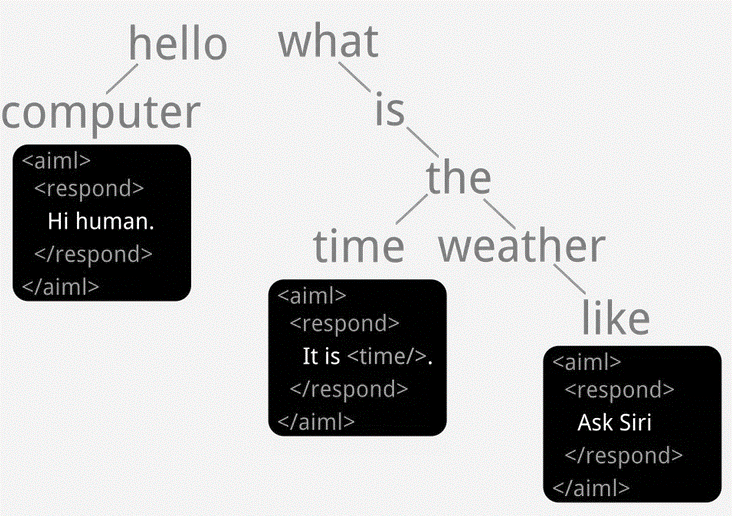
\includegraphics[width=0.8\textwidth]{./fig/image12.png} % Ajuste o caminho se necessário
    \label{fig:representacaovisualabstrata}
    \vspace{0.2cm} % Espaçamento opcional
    {\footnotesize 
	
	Retirado de \url{https://www.pandorabots.com/docs/aiml-fundamentals/}}
\end{figure}

O profissional responsável pela criação, manutenção e curadoria da base de conhecimento de um \emph{chatbot} AIML é denominado \emph{botmaster} \cite{Wallace2000}. Suas atribuições englobam a edição da base (frequentemente via ferramentas auxiliares), a análise de logs de diálogo para identificar padrões de interação e a subsequente criação ou refino de respostas. Este papel pode ser exercido por indivíduos com diferentes perfis, incluindo \emph{webmasters}, desenvolvedores, redatores, engenheiros ou outros interessados na construção de chatbots \cite{Wallace2000}.

Algumas implementações de interpretadores AIML podem incorporar capacidades rudimentares de compreensão semântica através do \emph{Resource Description Framework} (RDF)\footnote{\url{https://github.com/keiffster/program-y/wiki/RDF}}. O RDF é um padrão W3C para representação de informações na Web, usualmente por meio de triplas (sujeito-predicado-objeto) que descrevem relações entre entidades. No contexto AIML, RDF pode ser utilizado para armazenar e consultar fatos. Contudo, mesmo com tais adições, as capacidades linguísticas permanecem aquém da complexidade e do potencial gerativo da linguagem humana, conforme descrito por \cite{chomsky2002syntactic}.

Embora \cite{Hohn2019} argumente que o AIML padrão carece de um conceito explícito de "intenção" (\emph{intent}), similar ao encontrado em plataformas de \emph{Natural Language Understanding} (NLU), é possível emular o reconhecimento de intenções. Isso é tipicamente alcançado definindo categorias que representam "formas canônicas" ou "padrões atômicos" para uma intenção específica\footnote{\url{https://medium.com/pandorabots-blog/new-feature-visualize-your-aiml-26e33a590da1}}. Variações de entrada (e.g., "oi", "olá") podem ser mapeadas para uma categoria canônica (e.g., "saudação") usando a \emph{tag} \texttt{<srai>} (\emph{Symbolic Reduction Artificial Intelligence}), que redireciona o fluxo de processamento (ver Figura~\ref{fig:sodatagsrai}). Dessa forma, um \emph{chatbot} AIML pode gerenciar intenções distintas dentro de seu domínio, como realizar um pedido ou verificar o status de entrega.

\begin{figure}
    \centering
    \caption{Uso da tag \texttt{<srai>}}
    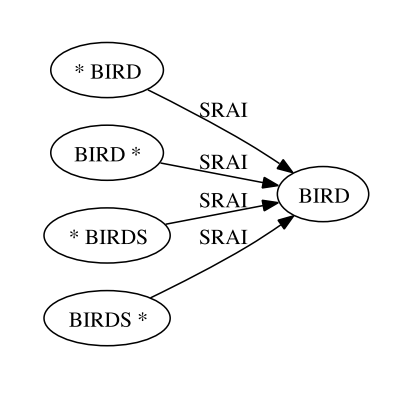
\includegraphics[width=0.5\textwidth]{./fig/image13.png} % Ajuste o caminho se necessário
    \label{fig:sodatagsrai}
    \vspace{0.2cm} % Espaçamento opcional
    {\footnotesize 
	
	Retirado de \cite{DeGasperis2013}}
\end{figure}

chatbots baseados em AIML têm obtido sucesso significativo em competições como o Prêmio Loebner. Notavelmente, o \emph{chatbot} Mitsuku\footnote{\url{https://www.pandorabots.com/mitsuku/}}, desenvolvido por Steve Worswick, conquistou múltiplos títulos recentes\footnote{\url{https://aisb.org.uk/category/loebner-prize/}}, seguindo vitórias anteriores do ALICE. \cite{Wallace2000}.

Adicionalmente, Mitsuku foi classificado em primeiro lugar numa análise comparativa envolvendo oito chatbots \cite{Sharma2020}. Nesse estudo, que avaliou atributos conversacionais com base em um conjunto padronizado de perguntas, o Google Assistant obteve a segunda posição, seguido pela Siri em terceiro. O \emph{chatbot} ALICE. alcançou a quarta posição, enquanto o ELIZA ficou na última colocação entre os sistemas comparados \cite{Sharma2020}.

\section{Tags do AIML 1.0: Explicação e Exemplos}

Esta seção descreve as principais tags do AIML, versão 1.0, com explicações e exemplos.

\paragraph{\texttt{<aiml>}} 

\textbf{Descrição:} Tag raiz que engloba todo o conteúdo AIML. 

\begin{lstlisting}
<aiml version="1.0">
	<!-- Categorias aqui -->
</aiml>
\end{lstlisting}

\paragraph{\texttt{<category>}} 

\textbf{Descrição:} Unidade básica de conhecimento, contendo um padrão e uma resposta. 

\begin{lstlisting}
<category>
	<pattern>OLÁ</pattern>
	<template>Oi! Como posso ajudar você hoje?</template>
</category>
\end{lstlisting}

\paragraph{\texttt{<pattern>}} 

\textbf{Descrição:} Define o padrão de entrada do usuário, com curingas como \texttt{*} e \texttt{\_}. 

\begin{lstlisting}
<category>
	<pattern>EU GOSTO DE *</pattern>
	<template>Que bom que você gosta de <star/>!</template>
</category>
\end{lstlisting}

\paragraph{\texttt{<template>}} 

\textbf{Descrição:} Define a resposta do bot ao padrão correspondente. 

\begin{lstlisting}
<category>
	<pattern>QUAL É O SEU NOME</pattern>
	<template>Meu nome é neo chatbot.</template>
</category> 
\end{lstlisting}

\paragraph{\texttt{<star/>}} 

\textbf{Descrição:} Captura o conteúdo do curinga \texttt{*} ou \texttt{\_}. 

\begin{lstlisting}
<category>
	<pattern>MEU NOME É *</pattern>
	<template>Olá, <star/>!</template>
</category>
\end{lstlisting}

\paragraph{\texttt{<that>}} 

\textbf{Descrição:} Considera a última resposta do bot para decidir a próxima. 

\begin{lstlisting}
<category>
	<pattern>SIM</pattern>
	<that>Você gosta de programar?</that>
	<template>Ótimo! Qual linguagem você prefere?</template>
</category>
\end{lstlisting}

\paragraph{\texttt{<topic>}} 

\textbf{Descrição:} Define um contexto ou tópico para categorias. 

\begin{lstlisting}
<category>
  <pattern>VAMOS FALAR SOBRE ESPORTE</pattern>
  <template>Ok! <topic name="esporte"/></template>
</category>
\end{lstlisting}

\paragraph{\texttt{<random>} e \texttt{<li>}} 

\textbf{Descrição:} Escolhe aleatoriamente uma resposta de uma lista. 

\begin{lstlisting}
<category>
  <pattern>COMO ESTÁ O TEMPO</pattern>
  <template>
    <random>
      <li>Está ensolarado!</li>
      <li>Está chovendo.</li>
    </random>
  </template>
</category>
\end{lstlisting}

\paragraph{\texttt{<condition>}} 

\textbf{Descrição:} Adiciona lógica condicional baseada em variáveis. 

\begin{lstlisting}
<category>
  <pattern>COMO EU ESTOU</pattern>
  <template>
    <condition name="humor">
      <li value="feliz">Você está bem!</li>
      <li>Não sei ainda!</li>
    </condition>
  </template>
</category>
\end{lstlisting}

\paragraph{\texttt{<set>} e \texttt{<get>}} 

\textbf{Descrição:} Define e recupera variáveis. 

\begin{lstlisting}
<category>
	<pattern>MEU NOME É *</pattern>
	<template><set name="nome"><star/></set>Olá, <get name="nome"/>!</template>
</category>
\end{lstlisting}

\paragraph{\texttt{<srai>}} 

\textbf{Descrição:} Redireciona a entrada para outro padrão. 

\begin{lstlisting}
<category>
	<pattern>OI</pattern>
	<template><srai>OLÁ</srai></template>
</category>
\end{lstlisting}

\paragraph{\texttt{<think>}} 

\textbf{Descrição:} Executa ações sem exibir o conteúdo. 

\begin{lstlisting}
<category>
	<pattern>EU SOU TRISTE</pattern>
	<template><think><set name="humor">triste</set></think>Sinto muito!</template>
</category>
\end{lstlisting}

\paragraph{\texttt{<person>}, \texttt{<person2>}, \texttt{<gender>}} 

\textbf{Descrição:} Transforma pronomes ou ajusta gênero. 

\begin{lstlisting}
<category>
	<pattern>EU TE AMO</pattern>
	<template><person><star/></person> ama você também!</template>
</category>
\end{lstlisting}

\paragraph{\texttt{<formal>}, \texttt{<uppercase>}, \texttt{<lowercase>}} 

\textbf{Descrição:} Formata texto (capitaliza, maiúsculas, minúsculas). 

\begin{lstlisting}
<category>
  <pattern>MEU NOME É joão</pattern>
  <template>Olá, <formal><star/></formal>!</template>
</category>
\end{lstlisting}

\paragraph{\texttt{<sentence>}} 

\textbf{Descrição:} Formata como frase (primeira letra maiúscula, ponto final). 

\begin{lstlisting}
<category>
  <pattern>oi</pattern>
  <template><sentence><star/></sentence></template>
</category>
\end{lstlisting}

\section{AIML exemplo em Python}

A seguir um exemplo do uso de um interpretador AIML em Python.

\vspace{\baselineskip}
\href{https://colab.research.google.com/github/giseldo/chatbotbook/blob/main/notebook/aiml/aiml1_1.ipynb}{
  
\includegraphics{./fig/colab-badge.png}
}

\begin{lstlisting}
# pip install aiml

import aiml

# Criar kernel (núcleo do bot)
kernel = aiml.Kernel()

# Carregar arquivos AIML
kernel.learn("std-startup.xml")
kernel.respond("LOAD AIML B")

# Loop de conversa
while True:
    user_input = input("Você: ")
    if user_input.lower() in ["sair", "exit", "quit"]:
        break
    response = kernel.respond(user_input)
    print("Bot:", response)
\end{lstlisting}

O arquivo std-startup.xml é um ponto de partida e geralmente carrega outros arquivos .aiml.

Estrutura básica de um arquivo .aiml:

\begin{lstlisting}
<aiml version="1.0.1" encoding="UTF-8">
  <category>
    <pattern>OI</pattern>
    <template>Olá! Como posso te ajudar?</template>
  </category>
  
  <category>
    <pattern>QUAL SEU NOME</pattern>
    <template>Eu sou um chatbot em AIML.</template>
  </category>
</aiml>
\end{lstlisting}

%%%%%%%%%%%%%%%%
%%%%CAPITULO%%%%
%%%%%%%%%%%%%%%%

\chapter{Processamento de Linguagem Natural}

Neste capítulo, vamos explorar os conceitos básicos de Processamento de Linguagem Natural (PLN), uma área da inteligência artificial que lida com a interação entre computadores e a linguagem humana. Veremos técnicas fundamentais como tokenização, lematização, stemização e remoção de stopwords. Além disso, vamos implementar essas técnicas utilizando as bibliotecas NLTK e SpaCy em Python.

\section{Introducão}

O \textbf{Processamento de Linguagem Natural (PLN)} é um campo  ligado à inteligência artificial, dedicando-se a equipar computadores com a capacidade de analisar e compreender a linguagem humana. 

Em um espectro mais amplo, o PLN engloba uma vasta gama de tarefas. Com PLN é possível manipular e analisar a linguagem natural, seja em sua forma escrita ou falada, com o intuito de concretizar tarefas específicas e úteis. Este processo envolve a decomposição da linguagem em unidades menores, a compreensão do seu significado intrínseco e a determinação da resposta ou ação mais adequada.

Na construção de \textit{chatbots} sua função principal reside em processar a entrada bruta do usuário, realizando a limpeza e a preparação dos dados textuais para que o sistema possa interpretar a mensagem e tomar as ações subsequentes apropriadas.

\section{Conceitos Básicos de PLN}

\subsection{Tokenização}

Tokenização é o processo de dividir um texto em unidades menores chamadas "tokens", que podem ser palavras, frases ou até mesmo sentenças. A tokenização é o primeiro passo em muitos algoritmos de PLN, pois permite que os dados textuais sejam manipulados de forma 
programática.

Este processo inicial segmenta o texto em unidades menores denominadas \textit{tokens}, que podem ser palavras, pontuações ou símbolos. A tokenização é um passo preparatório fundamental para qualquer análise linguística subsequente. 

Tokenizar não é só separar por espaços, mas também lidar com pontuações, contrações e outros aspectos que podem afetar a análise. Por exemplo, "não é" pode ser tokenizado como ["não", "é"] ou ["não", "é"], dependendo do contexto e da abordagem adotada. 

Um exemplo simples seria a frase "Eu estou feliz.", que seria tokenizada em ["Eu", "estou", "feliz", "."]. Não necessariamente uma palavra equivale a um token. Em alguns casos, como em palavras compostas ou expressões idiomáticas, um único token pode representar uma ideia ou conceito mais amplo. Por exemplo, "São Paulo" poderia ser considerado um único token em vez de dois ("São" e "Paulo"). 

Existem diferentes abordagens para tokenização, incluindo tokenização baseada em regras, onde padrões específicos são definidos para identificar tokens (geralmente utilizando expressão regular), e tokenização baseada em aprendizado de máquina, onde algoritmos aprendem a segmentar o texto com base em exemplos anteriores.

A tokenização pode ser feita de várias maneiras, dependendo do idioma e do objetivo da análise. Em inglês, por exemplo, a tokenização pode ser mais simples devido à estrutura gramatical, enquanto em idiomas como o chinês, onde não há espaços entre as palavras, a tokenização pode ser mais complexa.

%TODO explicar o que é NLTK

A seguir um exemplo do uso da biblioteca nltk e a tokenização de determinado texto, também chamado de corpus.

\vspace{\baselineskip}
\href{https://colab.research.google.com/github/giseldo/chatbotbook/blob/main/notebook/pln/pln1_1.ipynb}{
  
\includegraphics{./fig/colab-badge.png}
}

\begin{lstlisting}[language=Python]
# pip install nltk

import nltk
from nltk.tokenize import word_tokenize, sent_tokenize

# Exemplo de texto
texto = "Chatbots estão se tornando cada vez mais populares. Eles podem realizar muitas tarefas automaticamente."

# Tokenização em palavras
tokens_palavras = word_tokenize(texto)
print("Tokens de palavras:", tokens_palavras)

# Tokenização em sentenças
tokens_sentencas = sent_tokenize(texto)
print("Tokens de sentenças:", tokens_sentencas)
\end{lstlisting}

\begin{lstlisting}
Tokens de palavras: ['Chatbots', 'estão', 'se', 'tornando', 'cada', 'vez', 'mais', 'populares', '.', 'Eles', 'podem', 'realizar', 'muitas', 'tarefas', 'automaticamente', '.']
Tokens de sentenças: ['Chatbots estão se tornando cada vez mais populares.', 'Eles podem realizar muitas tarefas automaticamente.']
\end{lstlisting}


SpaCy é uma biblioteca poderosa para PLN que oferece uma interface fácil de usar e é altamente otimizada para processamento rápido. É possível também utilizar a biblioteca spacy, conforme códigos a seguir:

\vspace{\baselineskip}
\href{https://colab.research.google.com/github/giseldo/chatbotbook/blob/main/notebook/pln/pln1_1_2.ipynb}{
  
\includegraphics{./fig/colab-badge.png}
}

\begin{lstlisting}[language=Python]
# pip install spacy

# import os
# os.system("python -m spacy download pt_core_news_sm")

import spacy

# Carregar o modelo de linguagem em português
nlp = spacy.load("pt_core_news_sm")

# Exemplo de texto
texto = "Chatbots estão se tornando cada vez mais populares."

# Processando o texto
doc = nlp(texto)

# Tokenização
tokens = [token.text for token in doc]
print("Tokens:", tokens)
\end{lstlisting}

\begin{lstlisting}
Tokens: ['Chatbots', 'estão', 'se', 'tornando', 'cada', 'vez', 'mais', 'populares', '.']
\end{lstlisting}


\subsection{Lematização}

Lematização é o processo de reduzir palavras flexionadas ao seu lema, ou forma base. Diferente da stemização, a lematização leva em consideração o contexto e a gramática da palavra para obter a forma correta.

\vspace{\baselineskip}
\href{https://colab.research.google.com/github/giseldo/chatbotbook/blob/main/notebook/pln/pln1_2.ipynb}{
  
\includegraphics{./fig/colab-badge.png}
}

\begin{lstlisting}[language=Python]
# pip install nltk

# import nltk
# nltk.download('wordnet')

import nltk
from nltk.stem import WordNetLemmatizer

# Inicializando o lematizador
lemmatizer = WordNetLemmatizer()

# Exemplo de palavras
palavras = ["correndo", "correu", "corredores"]

# Lematização das palavras
lematizadas = [lemmatizer.lemmatize(palavra, pos='v') for palavra in palavras]
print("Palavras lematizadas:", lematizadas)
\end{lstlisting}

\begin{lstlisting}
Palavras lematizadas: ['correndo', 'correu', 'corredores']
\end{lstlisting}

Com spacy

\vspace{\baselineskip}
\href{https://colab.research.google.com/github/giseldo/chatbotbook/blob/main/notebook/pln/pln1_2_2.ipynb}{
  
\includegraphics{./fig/colab-badge.png}
}

\begin{lstlisting}[language=Python]
import spacy

# Carregar o modelo de linguagem em português
nlp = spacy.load("pt_core_news_sm")

# Exemplo de texto
texto = "Chatbots estão se tornando cada vez mais populares."

# Processando o texto
doc = nlp(texto)

tokens = [token.text for token in doc]
print("Tokens:", tokens)

lematizadas = [token.lemma_ for token in doc]
print("Palavras lematizadas:", lematizadas)
\end{lstlisting}

\begin{lstlisting}
Tokens: ['Chatbots', 'estão', 'se', 'tornando', 'cada', 'vez', 'mais', 'populares', '.']
Palavras lematizadas: ['chatbots', 'estar', 'se', 'tornar', 'cada', 'vez', 'mais', 'popular', '.']
\end{lstlisting}

\subsection{Stemização}

A stemização é o processo de reduzir as palavras às suas raízes ou "stems". É uma técnica mais simples que a lematização e, geralmente, não considera o contexto, o que pode levar a resultados menos precisos.

\vspace{\baselineskip}
\href{https://colab.research.google.com/github/giseldo/chatbotbook/blob/main/notebook/pln/pln1_3.ipynb}{
  
\includegraphics{./fig/colab-badge.png}
}

\begin{lstlisting}[language=Python]
from nltk.stem import PorterStemmer

# Inicializando o stemizador
stemmer = PorterStemmer()

# Exemplo de palavras
palavras = ["correndo", "correu", "corredores"]

# Stemização das palavras
stems = [stemmer.stem(palavra) for palavra in palavras]
print("Stems das palavras:", stems)
\end{lstlisting}

\begin{lstlisting}
Stems das palavras: ['correndo', 'correu', 'corredor']
\end{lstlisting}

\subsection{Stopwords}

Stopwords são palavras comuns em um idioma (como "o", "a", "e", "de", "que", etc.) que geralmente são removidas durante o pré-processamento de texto, pois não contribuem significativamente para o significado do texto. A remoção dessas palavras pode melhorar a eficácia de certos algoritmos de PLN, focando nas palavras mais informativas do texto.

\vspace{\baselineskip}
\href{https://colab.research.google.com/github/giseldo/chatbotbook/blob/main/notebook/pln/pln1_4.ipynb}{
  
\includegraphics{./fig/colab-badge.png}
}

\begin{lstlisting}[language=Python]
# pip install nltk

# import nltk
# nltk.download('stopwords')

from nltk import word_tokenize
from nltk.corpus import stopwords

# Carregar stopwords para o idioma português
stop_words = set(stopwords.words('portuguese'))

# Exemplo de texto
texto = "Chatbots estão se tornando cada vez mais populares."

# Removendo stopwords
tokens_sem_stopwords = [palavra for palavra in word_tokenize(texto) if palavra.lower() not in stop_words]
print("Texto sem stopwords:", tokens_sem_stopwords)
\end{lstlisting}

\begin{lstlisting}
Texto sem stopwords: ['Chatbots', 'tornando', 'cada', 'vez', 'populares', '.']
\end{lstlisting}

com Spacy: \\

\begin{lstlisting}[language=Python]
import spacy

# Carregar o modelo de linguagem em português
nlp = spacy.load("pt_core_news_sm")

# Exemplo de texto
texto = "Chatbots estão se tornando cada vez mais populares."

# Processando o texto
doc = nlp(texto)

tokens = [token.text for token in doc]
print("Tokens:", tokens)

# Removendo stopwords
tokens_sem_stopwords = [token.text for token in doc if not token.is_stop]
print("Texto sem stopwords:", tokens_sem_stopwords)
\end{lstlisting}
	
\subsection{Marcação Morfossintática (POS Tagging)}

Esta técnica consiste em atribuir a cada \textit{token} em um texto uma categoria gramatical, como substantivo, verbo, adjetivo, advérbio, etc.. A marcação POS é crucial para identificar entidades e compreender a estrutura gramatical das frases. Por exemplo, na frase "Eu estou aprendendo como construir chatbots", a marcação POS poderia identificar "Eu" como um pronome (PRON), "estou aprendendo" como um verbo (VERB) e "chatbots" como um substantivo (NOUN).

\subsection{Reconhecimento de Entidades Nomeadas (NER)}

O NER é a tarefa de identificar e classificar entidades nomeadas em um texto, como nomes de pessoas (PERSON), organizações (ORG), localizações geográficas (GPE, LOC), datas (DATE), valores monetários (MONEY), etc.. Por exemplo, na frase "Google tem sua sede em Mountain View, Califórnia, com uma receita de 109.65 bilhões de dólares americanos", o NER identificaria "Google" como uma organização (ORG), "Mountain View" e "Califórnia" como localizações geográficas (GPE) e "109.65 bilhões de dólares americanos" como um valor monetário (MONEY). Essa capacidade é vital para que \textit{chatbots} compreendam os detalhes relevantes nas \textit{utterances} dos usuários.

\subsection{Análise de Dependências (Dependency Parsing)}

Esta técnica examina as relações gramaticais entre as palavras em uma frase, revelando a estrutura sintática e as dependências entre os \textit{tokens}. A análise de dependências pode ajudar a entender quem está fazendo o quê a quem. Por exemplo, na frase "Reserve um voo de Bangalore para Goa", a análise de dependências pode identificar "Bangalore" e "Goa" como modificadores de "voo" através das preposições "de" e "para", respectivamente, e "Reserve" como a raiz da ação. Essa análise é útil para extrair informações sobre as intenções do usuário, mesmo em frases mais complexas.

\subsection{Identificação de Grupos Nominais (Noun Chunks)}

Esta técnica visa identificar sequências contínuas de palavras que atuam como um sintagma nominal. Grupos nominais representam entidades ou conceitos chave em uma frase. Um exemplo seria na frase "Boston Dynamics está se preparando para produzir milhares de cães robóticos", onde "Boston Dynamics" e "milhares de cães robóticos" seriam identificados como grupos nominais.

\subsection{Busca por Similaridade}

Utilizando vetores de palavras (\textit{word embeddings}), como os gerados pelo algoritmo GloVe, é possível calcular a similaridade semântica entre palavras ou frases. Essa técnica permite que \textit{chatbots} reconheçam que palavras diferentes podem ter significados relacionados. Por exemplo, "carro" e "caminhão" seriam considerados mais similares do que "carro" e "google". Isso é útil para lidar com a variedade de expressões que os usuários podem usar para expressar a mesma intenção.

\subsection{Expressões Regulares}

São padrões de texto que podem ser usados para corresponder a sequências específicas de caracteres. Embora não sejam uma técnica de PLN no mesmo sentido que as outras, as expressões regulares são ferramentas poderosas para identificar padrões em texto, como números de telefone, endereços de e-mail ou formatos específicos de entrada.

\subsection{Classificação de Texto}

Uma técnica de aprendizado de máquina que atribui um texto a uma ou mais categorias predefinidas. No contexto de \textit{chatbots}, a classificação de texto é fundamental para a detecção de intenção, onde as categorias representam as diferentes intenções do usuário. Algoritmos como o \textit{Naïve Bayes} são modelos estatísticos populares para essa tarefa, baseados no teorema de Bayes e em fortes suposições de independência entre as características. O treinamento desses classificadores requer um \textit{corpus} de dados rotulados, onde cada \textit{utterance} (entrada do usuário) é associada a uma intenção específica.


\section{Entendimento de Linguagem Natural (ULN) como Subconjunto do PLN}

O \textbf{Entendimento de Linguagem Natural (ULN)} é um subdomínio específico dentro do universo mais vasto do PLN. Enquanto o PLN abarca um conjunto diversificado de operações sobre a linguagem, o ULN se concentra de maneira particular na habilidade da máquina de apreender e interpretar a linguagem natural tal como ela é comunicada pelos seres humanos. 
Em outras palavras, o ULN é o ramo do PLN dedicado à extração de significado e à identificação da intenção por trás do texto inserido pelo usuário. As aplicações do ULN são extensas e incluem funcionalidades cruciais para \textit{chatbots}, como a capacidade de responder a perguntas, realizar buscas em linguagem natural, identificar relações entre entidades, analisar o sentimento expresso no texto, sumarizar informações textuais e auxiliar em processos de descoberta legal.

% A relação entre PLN e ULN é frequentemente ilustrada como um diagrama de Venn, onde o ULN se posiciona como um subconjunto do PLN. Essa representação sublinha que, embora o PLN englobe diversas técnicas de processamento da linguagem que não necessariamente envolvem a compreensão em profundidade do significado, o ULN se dedica especificamente à interpretação semântica do texto para que as máquinas possam, em alguma medida, "pensar" de maneira similar aos humanos.

\section{Técnicas Fundamentais de PLN para Chatbots}

A construção de \textit{chatbots} eficazes repousa sobre o emprego de diversas técnicas de PLN, cada uma contribuindo para a capacidade do sistema de interagir de forma inteligente com os usuários. 



\section{Ferramentas e Bibliotecas de PLN Populares}

\begin{itemize}
    \item \textbf{spaCy}: Uma biblioteca de PLN de código aberto em Python e Cython, conhecida por sua velocidade e eficiência. O spaCy oferece APIs intuitivas e modelos pré-treinados para diversas tarefas de PLN, incluindo tokenização, POS tagging, lematização, NER e análise de dependências. Sua arquitetura é focada em desempenho para aplicações em produção.
    \item \textbf{NLTK (Natural Language Toolkit)}: Uma biblioteca Python fundamental para PLN, oferecendo uma ampla gama de ferramentas e recursos para tarefas como tokenização, stemming, POS tagging, análise sintática e NER. O NLTK é frequentemente utilizado para fins educacionais e de pesquisa.
    \item \textbf{CoreNLP (Stanford CoreNLP)}: Um conjunto de ferramentas de PLN robusto e amplamente utilizado, desenvolvido em Java. O CoreNLP oferece capacidades abrangentes de análise linguística, incluindo POS tagging, análise de dependências, NER e análise de sentimentos. Possui APIs para integração com diversas linguagens de programação, incluindo Python.
    \item \textbf{gensim}: Uma biblioteca Python especializada em modelagem de tópicos, análise de similaridade semântica e vetores de palavras. O gensim é particularmente útil para identificar estruturas semânticas em grandes coleções de texto.
    \item \textbf{TextBlob}: Uma biblioteca Python mais simples, construída sobre NLTK e spaCy, que fornece uma interface fácil de usar para tarefas básicas de PLN, como POS tagging, análise de sentimentos e correção ortográfica.
    
	% \item \textbf{fastText}: Uma biblioteca desenvolvida pelo Facebook para aprendizado de representações de palavras e classificação de texto rápida. O fastText é eficaz no tratamento de palavras fora do vocabulário de treinamento.
	
    % \item \textbf{LUIS.ai (Language Understanding Intelligent Service)}: Uma plataforma da Microsoft Azure Cognitive Services para construir modelos de linguagem natural que podem entender as intenções dos usuários e extrair entidades de suas \textit{utterances}. LUIS utiliza técnicas de aprendizado de máquina para classificar intenções e reconhecer entidades.
    \item \textbf{Rasa NLU}: Um componente de código aberto do framework Rasa para construir \textit{chatbots}, focado em entendimento de linguagem natural. Rasa NLU permite treinar modelos personalizados para classificação de intenção e extração de entidades, oferecendo flexibilidade e controle sobre os dados.
\end{itemize}

\section{O Papel do PLN na Construção de Chatbots}

No cerne da funcionalidade de um \textit{chatbot} reside a sua capacidade de compreender as mensagens dos usuários e responder de forma adequada. O PLN desempenha um papel central nesse processo, permitindo que o \textit{chatbot}:

\begin{itemize}
    \item \textbf{Detecte a Intenção do Usuário}: Identificar o objetivo por trás da mensagem do usuário é o primeiro passo. Isso é frequentemente abordado como um problema de classificação de texto, onde o \textit{chatbot} tenta classificar a \textit{utterance} do usuário em uma das intenções predefinidas. Para detecção da intenção é possível utilziar técnicas de aprendizado de máquina, como o algoritmo \textit{Naïve Bayes}, para construir esses classificadores. Plataformas como LUIS.ai e Rasa NLU simplificam significativamente o processo de treinamento e implantação desses modelos de intenção.
    \item \textbf{Extraia Entidades Relevantes}: Além da intenção geral, as mensagens dos usuários frequentemente contêm detalhes específicos, conhecidos como entidades, que são essenciais para atender à solicitação. Por exemplo, em "Reserve um voo de Londres para Nova York amanhã", a intenção é reservar um voo, e as entidades são a cidade de origem ("Londres"), a cidade de destino ("Nova York") e a data ("amanhã"). As técnicas de NER e os modelos de extração de entidades fornecidos por ferramentas como spaCy, NLTK, CoreNLP, LUIS.ai e Rasa NLU são fundamentais para identificar e extrair essas informações cruciais.
    \item \textbf{Processe Linguagem Variada e Informal}: Os usuários podem se comunicar com \textit{chatbots} usando uma ampla gama de vocabulário, gramática e estilo, incluindo erros de digitação, abreviações e linguagem informal. As técnicas de PLN, como stemming, lematização e busca por similaridade, ajudam o \textit{chatbot} a lidar com essa variabilidade e a compreender a essência da mensagem, mesmo que não seja expressa de forma perfeitamente gramatical.
    \item \textbf{Mantenha o Contexto da Conversa}: Em conversas mais longas, o significado de uma \textit{utterance} pode depender do que foi dito anteriormente. O PLN, juntamente com outras técnicas de gerenciamento de diálogo, contribui para a capacidade do \textit{chatbot} de lembrar informações e entender referências implícitas.
\end{itemize}

\section{PLN na Arquitetura de Chatbots}

A arquitetura típica de um \textit{chatbot} envolve uma camada de processamento de linguagem natural (NLP/NLU engine) que recebe a entrada de texto do usuário. Essa camada é responsável por realizar as tarefas de PLN mencionadas anteriormente: tokenização, análise morfossintática, extração de entidades, detecção de intenção, etc.. O resultado desse processamento é uma representação estruturada da mensagem do usuário, que pode ser entendida pela lógica de negócios do \textit{chatbot}.

Com base nessa representação estruturada, um motor de decisão (\textit{decision engine}) no \textit{chatbot} pode então corresponder a intenção do usuário a fluxos de trabalho preconfigurados ou a regras de negócio específicas. Em alguns casos, a geração de linguagem natural (NLG), outro subcampo do PLN, é utilizada para formular a resposta do \textit{chatbot} ao usuário.

\section{Desafios da PLN}

\begin{itemize}
	\item Geração de Texto coerente
	\item Sintaxe e gramática
	\item semântica
	\item Contexto
	\item Ambiguidade
\end{itemize}

A Geração de Texto coerente é um desafio porque envolve não apenas a escolha de palavras, mas também a construção de frases que façam sentido no contexto da conversa. A sintaxe e gramática são importantes para garantir que o texto gerado seja gramaticalmente correto e compreensível. A semântica se refere ao significado das palavras e frases, e é importante para garantir que o texto gerado transmita a mensagem correta. O contexto é importante para entender o que foi dito anteriormente na conversa e como isso afeta a resposta atual. A ambiguidade pode surgir quando uma palavra ou frase tem múltiplos significados, tornando difícil para o modelo determinar qual interpretação é a correta.

\section{Conclusão}

Neste capítulo, cobrimos os fundamentos de Processamento de Linguagem Natural (PLN), incluindo tokenização, lematização, stemização e remoção de stopwords. Também vimos como implementar essas técnicas em Python utilizando as bibliotecas NLTK e SpaCy. Esses conceitos são essenciais para o desenvolvimento de sistemas de processamento de texto e serão a base para os tópicos mais avançados que abordaremos nos próximos capítulos.

\newpage

\section{Exercícios de Múltipla Escolha}

\begin{enumerate}
\item \textbf{O que é vetorização de texto no contexto de processamento de linguagem natural?} 
\begin{enumerate}[label=\alph*)]
\item A compressão de textos longos para reduzir o tamanho dos arquivos. 
\item A transformação de palavras ou documentos em representações numéricas. 
\item A categorização de textos em diferentes classes. 
\item A separação de um texto em frases ou parágrafos distintos. 
\end{enumerate}
%B

\item \textbf{Qual das seguintes técnicas de vetorização é baseada na frequência de termos em um documento?} 
\begin{enumerate}[label=\alph*)]
\item Word2Vec 
\item TF-IDF 
\item Bag of Words (BoW) 
\item Embeddings de Palavras 
\end{enumerate}
%B

\item \textbf{O que é a técnica Bag of Words (BoW)?} 
\begin{enumerate}[label=\alph*)]
\item Um método de combinar várias palavras em uma única representação vetorial. 
\item Um método de contar a frequência de palavras em um documento sem considerar a ordem das palavras. 
\item Um algoritmo de compressão de texto. 
\item Uma técnica para traduzir texto entre diferentes idiomas. 
\end{enumerate}
%B

\item \textbf{Qual das alternativas a seguir é uma desvantagem do modelo Bag of Words?} 
\begin{enumerate}[label=\alph*)]
\item Ele não consegue capturar a ordem das palavras. 
\item Ele é muito difícil de implementar. 
\item  Ele não suporta múltiplos idiomas. 
\item  Ele exige uma grande quantidade de dados para funcionar. 
\end{enumerate}
%A

\item \textbf{O que é um embedding de palavras?} 
\begin{enumerate}[label=\alph*)]
\item Uma matriz de números binários que representa a presença ou ausência de palavras em um texto. 
\item Um vetor de números que representa o significado semântico de uma palavra no contexto de um grande corpus de textos. 
\item Um conjunto de palavras agrupadas por temas semelhantes. 
\item Uma técnica para compactar arquivos de texto. 
\end{enumerate}
%B

\end{enumerate}

%%%%%%%%%%%%%%%%%%%%
%%%%%%CAPITULO%%%%%%
%%%%%%%%%%%%%%%%%%%%

\chapter{Intençãos e Entidades}
\label{chap:intents}

\section{Introdução}

Os Intents representam a intenção ou o propósito por trás da mensagem de um usuário ao interagir com o chatbot. Em termos mais simples, é o que o usuário deseja que o chatbot faça ou sobre o que ele quer saber.

\section{Definição e Propósito}
\label{sec:intents_definicao}

Um intent é usado para identificar programaticamente a intenção da pessoa que está usando o chatbot. O chatbot deve ser capaz de executar alguma ação com base no "intent" que detecta na mensagem do usuário. Cada tarefa que o chatbot deve realizar define um intent.

\section{Exemplos de Intents}
\label{sec:intents_exemplos}

A aplicação prática dos intents varia conforme o domínio do chatbot:
\begin{itemize}
    \item Para um chatbot de uma loja de moda, exemplos de intents seriam \texttt{busca de um produto} (quando um usuário quer ver produtos) e \texttt{endereço loja} (quando um usuário pergunta sobre lojas).
    \item Em um chatbot para pedir comida, \texttt{consultar preços} e \texttt{realizar pedido} podem ser intents distintos.
\end{itemize}

\section{Detecção de Intent}
\label{sec:intents_deteccao}

Detectar o intent da mensagem do usuário é um problema conhecido de aprendizado de máquina, realizado por meio de uma técnica chamada classificação de texto. O objetivo é classificar frases em múltiplas classes (os intents). O modelo de aprendizado de máquina é treinado com um conjunto de dados que contém exemplos de mensagens e seus intents correspondentes. Após o treinamento, o modelo pode prever o intent de novas mensagens que não foram vistas antes.

\section{Utterances (Expressões do Usuário)}
\label{sec:intents_utterances}

Cada intent pode ser expresso de várias maneiras pelo usuário. Essas diferentes formas são chamadas de \textit{utterances} ou expressões do usuário. 

Por exemplo, para o intent \texttt{realizar pedido}, as utterances poderiam ser ""Eu gostaria de fazer um pedido", "Quero pedir comida", "Como faço para pedir?", etc. Cada uma dessas expressões representa a mesma intenção, mas com palavras diferentes. O modelo de aprendizado de máquina deve ser capaz de reconhecer todas essas variações como pertencentes ao mesmo intent.

É sugerido fornecer um número ótimo de utterances variadas por intent para garantir um bom treinamento do modelo de reconhecimento.

\section{Entities (Entidades)}
\label{sec:intents_entities}

Os Intents frequentemente contêm metadados importantes chamados \textit{Entities}. Estas são palavras-chave ou frases dentro da utterance do usuário que ajudam o chatbot a identificar detalhes específicos sobre o pedido, permitindo fornecer informações mais direcionadas. Por exemplo, na frase "Eu quero pedir uma pizza de calabreza com borda rechada", as entidades podem incluir:
\begin{itemize}
	\item O \textbf{Intent} é \texttt{realizar pedido}.
	\item As \textbf{Entities} podem ser: \texttt{pizza}, \texttt{calabreza}, \texttt{borda recheada}.
\end{itemize}

As entidades extraídas permitem ao chatbot refinar sua resposta ou ação.

\section{Treinamento do Bot}
\label{sec:intents_treinamento}

O processo de treinamento envolve a construção de um modelo de aprendizado de máquina. Este modelo aprende a partir do conjunto definido de intents, suas utterances associadas e as entidades anotadas. O objetivo do treinamento é capacitar o modelo a categorizar corretamente novas utterances (que não foram vistas durante o treinamento) no intent apropriado e a extrair as entidades relevantes.

\section{Pontuação de Confiança (Confidence Score)}
\label{sec:intents_confianca}

Quando o chatbot processa uma nova mensagem do usuário, o modelo de reconhecimento de intent não apenas classifica a mensagem em um dos intents definidos, mas também fornece uma \textit{pontuação de confiança} (geralmente entre 0 e 1). Essa pontuação indica o quão seguro o modelo está de que a classificação está correta. É comum definir um \textit{limite (threshold)} de confiança. Se a pontuação do intent detectado estiver abaixo desse limite, o chatbot pode pedir esclarecimentos ao usuário em vez de executar uma ação baseada em uma suposição incerta.

\section{Uso Prático e Análise}
\label{sec:intents_uso_pratico}

Uma vez que um intent é detectado com confiança suficiente, o chatbot pode executar a ação correspondente. Isso pode envolver consultar um banco de dados, chamar uma API externa, fornecer uma resposta estática ou iniciar um fluxo de diálogo mais complexo. Além disso, a análise dos intents mais frequentemente capturados fornece insights valiosos sobre como os usuários estão interagindo com o chatbot e quais são suas principais necessidades. Essas análises são importantes tanto para a otimização do bot quanto para as decisões de negócio.

\section{Resumo e Relação com Outros Conceitos}
\label{sec:intents_resumo}

Em resumo, Intents são um conceito central na arquitetura de chatbots modernos baseados em NLU (Natural Language Understanding). Eles representam o objetivo do usuário e permitem que o chatbot compreenda a intenção por trás das mensagens para agir de forma adequada. Os Intents estão intrinsecamente ligados a outros conceitos fundamentais:
\begin{itemize}
    \item \textbf{Entities:} Fornecem os detalhes específicos dentro de um intent.
    \item \textbf{Utterances:} São as diversas maneiras como um usuário pode expressar um mesmo intent.
    \item \textbf{Actions/Responses:} São as tarefas ou respostas que o chatbot executa após identificar um intent.
\end{itemize}
A definição cuidadosa, o treinamento robusto e o gerenciamento contínuo dos intents são cruciais para a eficácia, a inteligência e a qualidade da experiência do usuário oferecida por um chatbot.

%%%%%%%%%%%%%%%%
%%%%CAPITULO%%%%
%%%%%%%%%%%%%%%%

\chapter{LLM}

\section{Introdução}

Os Modelos de Linguagem de Grande Escala, conhecidos como Large Language Models (LLMs), são sistemas avançados de inteligência artificial projetados para compreender, gerar e manipular linguagem natural de forma sofisticada. Esses modelos são alimentados por vastos conjuntos de dados textuais e utilizam técnicas de aprendizado profundo, particularmente redes neurais, para aprender padrões, contextos e nuances da linguagem.

Os LLMs são capazes de realizar uma variedade de tarefas linguísticas, incluindo tradução automática, geração de texto, resumo de informações, resposta a perguntas e até mesmo a criação de diálogos interativos. Eles funcionam com base em arquiteturas complexas, como a Transformer, que permite que o modelo preste atenção a diferentes partes de um texto simultaneamente, facilitando a compreensão do contexto e das relações semânticas entre palavras e frases.

O treinamento desses modelos envolve a exposição a enormes quantidades de texto, o que lhes permite desenvolver uma compreensão profunda da gramática, do vocabulário e dos estilos de comunicação. No entanto, essa capacidade de gerar texto coerente e relevante também levanta questões éticas e de responsabilidade, especialmente em relação à desinformação, viés algorítmico e privacidade.

Em resumo, os Modelos de Linguagem de Grande Escala representam um marco significativo na evolução da inteligência artificial, oferecendo ferramentas poderosas para a interação humano-computador e abrindo novas possibilidades para aplicações em diversas áreas, como educação, atendimento ao cliente, criação de conteúdo e muito mais.

%%%%%%%%%%%%%%%%%%%%
%%%%%%CAPITULO%%%%%%
%%%%%%%%%%%%%%%%%%%%

\chapter{Retrieval-Augmented Generation}

\section{Introdução}

Retrieval Augmented Generation (RAG) é uma abordagem inovadora que combina duas técnicas fundamentais na área de processamento de linguagem natural: recuperação de informações e geração de texto. A ideia central do RAG é aprimorar a capacidade de um modelo de linguagem ao integrá-lo com um sistema de recuperação que busca informações relevantes de uma base de dados ou de um conjunto de documentos.

Na prática, o RAG opera em duas etapas principais. Primeiro, quando uma consulta ou pergunta é feita, um mecanismo de recuperação é acionado para identificar e extrair informações pertinentes de um repositório de dados. Isso pode incluir documentos, artigos, ou qualquer outro tipo de conteúdo textual que possa fornecer contexto e detalhes adicionais sobre o tema em questão. Essa fase garante que o modelo de linguagem tenha acesso a informações atualizadas e específicas, em vez de depender apenas do conhecimento prévio que foi incorporado durante seu treinamento.

Em seguida, na segunda etapa, o modelo de linguagem utiliza as informações recuperadas para gerar uma resposta mais rica e contextualizada. Essa geração não se limita a reproduzir o conteúdo recuperado, mas sim a integrar esses dados de forma coesa, criando uma resposta que não apenas responde à pergunta, mas também fornece uma narrativa mais completa e informativa. Isso resulta em respostas que são mais precisas e relevantes, pois são fundamentadas em dados concretos e atualizados.

A combinação dessas duas etapas permite que o RAG supere algumas limitações dos modelos de linguagem tradicionais, que podem falhar em fornecer informações precisas ou atualizadas, especialmente em domínios que evoluem rapidamente. Além disso, essa abordagem é particularmente útil em aplicações como assistentes virtuais, chatbots e sistemas de perguntas e respostas, onde a precisão e a relevância da informação são cruciais para a experiência do usuário.

Em resumo, o Retrieval Augmented Generation é uma técnica poderosa que não apenas melhora a qualidade das respostas geradas por modelos de linguagem, mas também amplia o alcance e a aplicabilidade desses modelos em cenários do mundo real, onde a informação é dinâmica e em constante evolução.

%%%%%%%%%%%%%%%%
%%%%CAPITULO%%%%
%%%%%%%%%%%%%%%%


%%%%%%%%%%%%%%%%
%%%%CAPITULO%%%%
%%%%%%%%%%%%%%%%

\chapter{LangChain}

\section{Introdução}

LangChain é uma biblioteca de software de código aberto projetada para simplificar a interação com Large Language Models (LLMs) e construir aplicativos de processamento de linguagem natural robustos. Ele fornece uma camada de abstração de alto nível sobre as complexidades de trabalhar diretamente com modelos de linguagem, tornando mais acessível a criação de aplicativos de compreensão e geração de linguagem.

\section{Por que usar LangChain?}

Trabalhar com LLMs pode ser complexo devido à sua natureza sofisticada e aos requisitos de recursos computacionais. LangChain lida com muitos detalhes complexos em segundo plano, permitindo que os desenvolvedores se concentrem na construção de aplicativos de linguagem eficazes. Aqui estão algumas vantagens do uso do LangChain:

\begin{itemize}
    \item Simplicidade: LangChain oferece uma API simples e intuitiva, ocultando os detalhes complexos de interação com LLMs. Ele abstrai as nuances de carregar modelos, gerenciar recursos computacionais e executar previsões.
    
    \item Flexibilidade: A biblioteca suporta vários frameworks de deep learning, como TensorFlow e PyTorch, e pode ser integrada a diferentes LLMs. Isso oferece aos desenvolvedores a flexibilidade de escolher as ferramentas e modelos que melhor atendem às suas necessidades.
    
    \item Extensibilidade: LangChain é projetado para ser extensível, permitindo que os usuários criem seus próprios componentes personalizados. Você pode adicionar novos modelos, adaptar o processamento de texto ou desenvolver recursos específicos do domínio para atender aos requisitos exclusivos do seu aplicativo.
    
    \item Comunidade e suporte: LangChain tem uma comunidade ativa de desenvolvedores e pesquisadores que contribuem para o projeto. A documentação abrangente, tutoriais e suporte da comunidade tornam mais fácil começar e navegar por quaisquer desafios que surgirem durante o desenvolvimento.
    
\end{itemize}
\section{Arquitetura do LangChain}

A arquitetura do LangChain pode ser entendida em três componentes principais:

Camada de Abstração: Esta camada fornece uma interface simples e unificada para interagir com diferentes LLMs. Ele abstrai as complexidades de carregar, inicializar e executar previsões em modelos, oferecendo uma API consistente independentemente do modelo subjacente.

Camada de Processamento de Texto: O LangChain inclui ferramentas robustas para processamento de texto, incluindo tokenização, análise sintática, reconhecimento de entidades nomeadas (NER) e muito mais. Esta camada prepara os dados de entrada e saída para que possam ser processados de forma eficaz pelos modelos de linguagem.

Camada de Modelo: Aqui é onde os próprios LLMs residem. O LangChain suporta uma variedade de modelos de linguagem, desde modelos pré-treinados de uso geral até modelos personalizados específicos de domínio. Esta camada lida com a execução de previsões, gerenciamento de recursos computacionais e interação com as APIs dos modelos.

\section{Exemplo Básico: Consultando um LLM}

Vamos ver um exemplo simples de como usar o LangChain para consultar um LLM e obter uma resposta. Neste exemplo, usaremos o gpt-4o-mini da OpenAI, para responder a uma pergunta.

Primeiro, importe as bibliotecas necessárias e configure o cliente LangChain. Em seguida, carregue o modelo de linguagem desejado. Agora, você pode usar o modelo para fazer uma consulta. Vamos perguntar quem é o presidente do Brasil.

\vspace{\baselineskip}
\href{https://colab.research.google.com/github/giseldo/chatbotbook/blob/main/notebook/cap9.ipynb}{
  
\includegraphics{./fig/colab-badge.png}
}

\begin{lstlisting}[language=Python, caption=Exemplo de uso do LangChain]
from langchain.chat_models import init_chat_model
from langchain_core.messages import HumanMessage
import os

OPENAI_API_KEY = os.environ.get("OPENAI_API_KEY")

model = init_chat_model("gpt-4o-mini", model_provider="openai", 						openai_api_key=OPENAI_API_KEY)

user_message = HumanMessage(content="Quem é o presidente do Brasil?")

response = model.invoke([user_message])

print(response.content)
\end{lstlisting}

\begin{lstlisting}
Até a minha última atualização em outubro de 2023, o presidente do Brasil é Luiz Inácio Lula da Silva. Ele assumiu o cargo em janeiro de 2023. Para informações mais atualizadas, recomendo verificar fontes de notícias recentes.
\end{lstlisting}

Este exemplo básico demonstra a simplicidade de usar o LangChain para interagir com LLMs. No entanto, o LangChain oferece muito mais recursos e funcionalidades para construir aplicativos de chatbot mais robustos.

%%%%%%%%%%%%%%%%
%%%%CAPITULO%%%%
%%%%%%%%%%%%%%%%

\chapter{Fluxos em LLM}

\section{Introdução}

Modelos de Linguagem Grandes (LLMs), como a família GPT, são incrivelmente poderosos na compreensão e geração de texto. Uma maneira eficaz e relativamente rápida de criar um chatbot funcional é através da \textbf{engenharia de prompts}. Em vez de codificar regras complexas e árvores de decisão manualmente, você "programa" o LLM fornecendo-lhe um conjunto detalhado de instruções iniciais (o prompt).

\section{Introdução}

O prompt é o texto inicial que você fornece ao LLM. Ele define:

\begin{enumerate}
    \item \textbf{O Papel do Chatbot:} Quem ele é (um atendente de pizzaria, um consultor de moda, etc.).
    \item \textbf{O Objetivo da Conversa:} O que ele precisa alcançar (vender uma pizza, ajudar a escolher uma roupa, abrir uma conta, etc.).
    \item \textbf{As Regras da Conversa:} A sequência exata de perguntas a fazer, as opções válidas para cada pergunta, e como lidar com diferentes respostas do usuário (lógica condicional).
    \item \textbf{O Tom e Estilo:} Se o chatbot deve ser formal, informal, amigável, etc. (embora não especificado nos exemplos, pode ser adicionado).
    \item \textbf{O Formato da Saída Final:} Como as informações coletadas devem ser apresentadas no final.
\end{enumerate}

\section*{Como Funciona?}

\begin{enumerate}
    \item \textbf{Definição:} Você escreve um prompt detalhado que descreve o fluxo da conversa passo a passo.
    \item \textbf{Instrução:} Você alimenta este prompt no LLM.
    \item \textbf{Execução:} O LLM usa o prompt como seu guia mestre. Ele inicia a conversa com o usuário seguindo o primeiro passo definido no prompt, faz as perguntas na ordem especificada, valida as respostas (se instruído), segue os caminhos condicionais e, finalmente, gera a saída desejada.
    \item \textbf{Iteração:} Se o chatbot não se comportar exatamente como esperado, você ajusta e refina o prompt até que ele siga as regras perfeitamente.
\end{enumerate}

\section*{Vantagens:}

\begin{itemize}
    \item \textbf{Rapidez:} Muito mais rápido do que desenvolver um chatbot tradicional do zero.
    \item \textbf{Flexibilidade:} Fácil de modificar o comportamento alterando o prompt.
    \item \textbf{Capacidade Conversacional:} Aproveita a habilidade natural do LLM para conversas fluidas.
\end{itemize}

\section*{Limitações:}

\begin{itemize}
    \item \textbf{Controle Fino:} Pode ser mais difícil garantir que sempre siga exatamente um caminho lógico muito complexo, embora prompts detalhados minimizem isso.
    \item \textbf{Estado:} Gerenciar estados complexos ao longo de conversas muito longas pode exigir técnicas de prompt mais avançadas.
\end{itemize}

\section*{Exemplos}

Dados os requisitos de negócio a seguir iremos implementar os chatbots utilizanddo LLM. \\

\textbf{1 Pizzaria} \\

\begin{itemize}[nosep]
	\item Construa um chatbot para uma pizzaria. O chatbot será responsável por vender uma pizza.
	\item Verifique com o usuário qual o o tipo de massa desejado da pizza (pan ou fina).
	\item Verifique o recheio (queijo, calabresa ou bacon)
	\item Se o usuário escolheu massa pan verifique qual o recheio da borda (gorgonzola ou cheddar)
	\item Ao final deve ser exibido as opções escolhidas.
\end{itemize} 

\vspace{\baselineskip}

\textbf{2 Loja de Roupas} \\

\begin{itemize}[nosep]
	\item Construa um chatbot para uma loja de roupas, o chatbot será responsável por vender uma calça ou camisa.
	\item Verifique se o usuário quer uma calça ou uma camisa.
	\item Se o usuário quiser uma calça:
	\item pergunte o tamanho da calça (34, 35 ou 36)
	\item pergunte o tipo de fit da calça pode ser slim fit, regular fit, skinny fit.
	\item Se ele quiser uma camisa:
	\item verifique se a camisa é (P, M ou g)
	\item verifique se ele deseja gola (v, redonda ou polo).
	\item Ao final informe as opções escolhidas com uma mensagem informando que o pedido está sendo processado.
\end{itemize} 

\vspace{\baselineskip}

\textbf{3 Empresa de Turismo} \\

\begin{itemize}[nosep]
	\item Este chatbot deve ser utilizado por uma empresa de turismo para vender um pacote turístico
	\item Verifique com o usuário quais das cidades disponíveis ele quer viajar (maceio, aracaju ou fortaleza)
	\item Se ele for para maceio:
	\item verifique se ele já conhece as belezas naturais da cidade.
	\item sugira os dois pacotes (nove ilhas e orla de alagoas)
	\item Se ele for a aracaju:
	\item verifique com o usuário quais dos dois passeios disponíveis serão escolhidos. existem duisponíveis um na passarela do carangueijo e outro na orla de aracaju.
	\item informe que somente existe passagem de ônibus e verifique se mesmo assim ele quer continuar
	\item Caso ele deseje ir a fortaleza:
	\item informe que o único pacote são as falasias cearenses.
	\item verifique se ele irá de ônibus ou de avião para o ceará
	\item Verifique a forma de pagamento cartão ou débito em todas as opções.
	\item Ao final informe as opções escolhidas com uma mensagem informando que o pedido está sendo processado.
\end{itemize} 

\vspace{\baselineskip}

\textbf{4 Banco Financeiro} \\

\begin{itemize}[nosep]
	\item Crie uma aplicação para um banco que será responsável por abrir uma conta corrente para um usuário.
	\item Verifique se o usuário já tem conta em outros bancos.
	\item Caso o usuário tenha conta em outros bancos verifique se ele quer fazer portabilidade
	\item Verifique o nome do correntista.
	\item Verifique qual o saldo que será depositado, zero ou um outro valor inicial.
	\item Verifique se o usuário quer um empréstimo.
	\item Ao final informe o nome do correntista, se ele quis um empréstimo e se ele fez portabilidade e o valor inicial da conta.
\end{itemize} 

\vspace{\baselineskip}

\textbf{5 Universidade} \\

\begin{itemize}[nosep]
	\item Desenvolver um chatbot para realização de matricula em duas disciplinas eletivas.
	\item O chatbot apresenta as duas disciplinas eletivas (Inteligência artificial Avançado, Aprendizagem de Máquina)
	\item Verificar se ele tem o pré-requisito introdução a programação para ambas as disciplinas.
	\item Se ele escolher Inteligência artificial avançada necessário confirmar se ele cursou inteligência artificial.
	\item Ao final informe qual o nome das disciplina em que ele se matriculou.
\end{itemize} 

\vspace{\baselineskip}

\textbf{Aplicando aos Exemplos:} \\

A seguir, mostramos como os fluxos de conversa do exercício anterior podem ser traduzidos em prompts para um LLM. Cada prompt instrui o modelo a agir como o chatbot específico e seguir as regras definidas.

\vspace{\baselineskip}

\textbf{Exemplos de Prompts} \\

\textbf{Exemplo 1: Pizzaria} \\

\textbf{Prompt para o LLM:} \\

\begin{lstlisting}
Você é um chatbot de atendimento de uma pizzaria. Sua tarefa é anotar o pedido de pizza de um cliente. 

Não responda nada fora deste contexto. Diga que não sabe.

Siga EXATAMENTE estes passos:

1.  Pergunte ao cliente qual o tipo de massa desejado. As únicas opções válidas são "pan" ou "fina".
    * Exemplo de pergunta: "Olá! Qual tipo de massa você prefere para sua pizza: pan ou fina?"
2.  Depois que o cliente escolher a massa, pergunte qual o recheio desejado. As únicas opções válidas são "queijo", "calabresa" ou "bacon".
    * Exemplo de pergunta: "Ótima escolha! E qual recheio você gostaria: queijo, calabresa ou bacon?"
3.  APENAS SE o cliente escolheu a massa "pan" no passo 1, pergunte qual o recheio da borda. As únicas opções válidas são "gorgonzola" ou "cheddar".
    * Exemplo de pergunta (apenas para massa pan): "Para a massa pan, temos borda recheada! Você prefere com gorgonzola ou cheddar?"
4.  Após coletar todas as informações necessárias (massa, recheio e recheio da borda, se aplicável), exiba um resumo claro do pedido com todas as opções escolhidas pelo cliente.
    * Exemplo de resumo: "Perfeito! Seu pedido ficou assim: Pizza com massa [massa escolhida], recheio de [recheio escolhido] [se aplicável: e borda recheada com [recheio da borda escolhido]]."

Inicie a conversa agora seguindo o passo 1.

\end{lstlisting}

\vspace{\baselineskip}
	
\textbf{Exemplo 2: Loja de Roupas} \\

\textbf{Prompt para o LLM:} \\

\begin{lstlisting}

Você é um chatbot de vendas de uma loja de roupas. Seu objetivo é ajudar o cliente a escolher uma calça ou uma camisa. 

Não responda nada fora deste contexto. Diga que não sabe.

Siga EXATAMENTE estes passos:

1.  Pergunte ao cliente se ele está procurando por uma "calça" ou uma "camisa".
	* Exemplo de pergunta: "Bem-vindo(a) à nossa loja! Você está procurando por uma calça ou uma camisa hoje?"
2.  SE o cliente responder "calça":
	a.  Pergunte o tamanho da calça. As únicas opções válidas são "34", "35" ou "36".
		* Exemplo de pergunta: "Para calças, qual tamanho você usa: 34, 35 ou 36?"
	b.  Depois do tamanho, pergunte o tipo de fit da calça. As únicas opções válidas são "slim fit", "regular fit" ou "skinny fit".
		* Exemplo de pergunta: "E qual tipo de fit você prefere: slim fit, regular fit ou skinny fit?"
3.  SE o cliente responder "camisa":
	a.  Pergunte o tamanho da camisa. As únicas opções válidas são "P", "M" ou "G".
		* Exemplo de pergunta: "Para camisas, qual tamanho você prefere: P, M ou G?"
	b.  Depois do tamanho, pergunte o tipo de gola. As únicas opções válidas são "V", "redonda" ou "polo".
		* Exemplo de pergunta: "E qual tipo de gola você gostaria: V, redonda ou polo?"
4.  Após coletar todas as informações (tipo de peça e suas especificações), apresente um resumo das opções escolhidas e informe que o pedido está sendo processado.
	* Exemplo de resumo (Cal\c{c}a): "Entendido! Voc\^e escolheu uma cal\c{c}a tamanho [tamanho] com fit [fit]. Seu pedido est\'a sendo processado."
	* Exemplo de resumo (Camisa): "Entendido! Você escolheu uma camisa tamanho [tamanho] com gola [gola]. Seu pedido está sendo processado."
	

Inicie a conversa agora seguindo o passo 1.
\end{lstlisting}

\vspace{\baselineskip}

\textbf{Exemplo 3: Empresa de Turismo} \\

\textbf{Prompt para o LLM:} \\

\begin{lstlisting}
Você é um agente de viagens virtual de uma empresa de turismo. Sua tarefa é ajudar um cliente a escolher e configurar um pacote turístico. 

Não responda nada fora deste contexto. Diga que não sabe.

Siga EXATAMENTE estes passos:

1.  Pergunte ao cliente para qual das cidades disponíveis ele gostaria de viajar. As únicas opções são "Maceió", "Aracaju" ou "Fortaleza".
    * Exemplo de pergunta: "Olá! Temos ótimos pacotes para Maceió, Aracaju e Fortaleza. Qual desses destinos te interessa mais?"
2.  SE o cliente escolher "Maceió":
    a.  Pergunte se ele já conhece as belezas naturais da cidade. (A resposta não altera o fluxo, é apenas conversacional).
        * Exemplo de pergunta: "Maceió é linda! Você já conhece as belezas naturais de lá?"
    b.  Sugira os dois pacotes disponíveis: "Nove Ilhas" e "Orla de Alagoas". Pergunte qual ele prefere.
        * Exemplo de pergunta: "Temos dois pacotes incríveis em Maceió: 'Nove Ilhas' e 'Orla de Alagoas'. Qual deles você prefere?"
    c.  Vá para o passo 5.
3.  SE o cliente escolher "Aracaju":
    a.  Pergunte qual dos dois passeios disponíveis ele prefere: "Passarela do Caranguejo" ou "Orla de Aracaju".
        * Exemplo de pergunta: "Em Aracaju, temos passeios pela 'Passarela do Caranguejo' e pela 'Orla de Aracaju'. Qual te atrai mais?"
    b.  Informe ao cliente que para Aracaju, no momento, só temos transporte via ônibus. Pergunte se ele deseja continuar mesmo assim.
        * Exemplo de pergunta: "Importante: para Aracaju, nosso transporte é apenas de ônibus. Podemos continuar com a reserva?"
    c.  Se ele confirmar, vá para o passo 5. Se não, agradeça e encerre.
4.  SE o cliente escolher "Fortaleza":
    a.  Informe que o pacote disponível é o "Falésias Cearenses".
        * Exemplo de informação: "Para Fortaleza, temos o pacote especial 'Falésias Cearenses'."
    b.  Pergunte se ele prefere ir de "ônibus" ou "avião" para o Ceará.
        * Exemplo de pergunta: "Como você prefere viajar para o Ceará: de ônibus ou avião?"
    c.  Vá para o passo 5.
5.  Depois de definir o destino, pacote/passeio e transporte (se aplicável), pergunte qual a forma de pagamento preferida. As únicas opções são "cartão" ou "débito".
    * Exemplo de pergunta: "Para finalizar, como você prefere pagar: cartão ou débito?"
6.  Ao final, apresente um resumo completo das opções escolhidas (destino, pacote/passeio, transporte se aplicável, forma de pagamento) e informe que o pedido está sendo processado.
    * Exemplo de resumo: "Confirmado! Seu pacote para [Destino] inclui [Pacote/Passeio], transporte por [Ônibus/Avião, se aplicável], com pagamento via [Forma de Pagamento]. Seu pedido está sendo processado!"

Inicie a conversa agora seguindo o passo 1.
\end{lstlisting}

\vspace{\baselineskip}

\textbf{Exemplo 4: Banco Financeiro} \\

\textbf{Prompt para o LLM:} \\

\begin{lstlisting}
Você é um assistente virtual de um banco e sua função é auxiliar usuários na abertura de uma conta corrente. 

Não responda nada fora deste contexto. Diga que não sabe.

Siga EXATAMENTE estes passos:

1.  Pergunte ao usuário se ele já possui conta em outros bancos. Respostas esperadas: "sim" ou "não".
	* Exemplo de pergunta: "Bem-vindo(a) ao nosso banco! Para começar, você já possui conta corrente em alguma outra instituição bancária?"
2.  APENAS SE a resposta for "sim", pergunte se ele gostaria de fazer a portabilidade da conta para o nosso banco. Respostas esperadas: "sim" ou "não".
	* Exemplo de pergunta: "Entendido. Você gostaria de solicitar a portabilidade da sua conta existente para o nosso banco?"
3.  Pergunte o nome completo do futuro correntista.
	* Exemplo de pergunta: "Por favor, informe o seu nome completo para o cadastro."
4.  Pergunte qual será o valor do depósito inicial na conta. Informe que pode ser "zero" ou qualquer outro valor.
	* Exemplo de pergunta: "Qual valor você gostaria de depositar inicialmente? Pode ser R$ 0,00 ou outro valor à sua escolha."
5.  Pergunte se o usuário tem interesse em solicitar um empréstimo pré-aprovado junto com a abertura da conta. Respostas esperadas: "sim" ou "não".
	* Exemplo de pergunta: "Você teria interesse em verificar uma oferta de empréstimo pré-aprovado neste momento?"
6.  Ao final, apresente um resumo com as informações coletadas: nome do correntista, se solicitou portabilidade (sim/não), se solicitou empréstimo (sim/não) e o valor do depósito inicial.
	* Exemplo de resumo: "Perfeito! Finalizamos a solicitação. Resumo da abertura: Correntista: [Nome Completo], Portabilidade Solicitada: [Sim/Não], Empréstimo Solicitado: [Sim/Não], Depósito Inicial: R$ [Valor]."

Inicie a conversa agora seguindo o passo 1.
\end{lstlisting}

\vspace{\baselineskip}

\textbf{Exemplo 5: Universidade} 

\textbf{Prompt para o LLM:} \\

\begin{lstlisting}[language=Tex]

Você é um assistente de matrícula de uma universidade. Sua tarefa é ajudar um aluno a se matricular em até duas disciplinas eletivas. 

Não responda nada fora deste contexto. Diga que não sabe.

Siga EXATAMENTE estes passos:

1.  Apresente as duas disciplinas eletivas disponíveis: "Inteligência Artificial Avançado" e "Aprendizagem de Máquina".
    * Exemplo de apresentação: "Olá! Temos duas disciplinas eletivas disponíveis para matrícula: 'Inteligência Artificial Avançado' e 'Aprendizagem de Máquina'."
2.  Verifique se o aluno possui o pré-requisito obrigatório "Introdução à Programação", que é necessário para AMBAS as disciplinas. Pergunte se ele já cursou e foi aprovado nesta disciplina. Respostas esperadas: "sim" ou "não".
    * Exemplo de pergunta: "Para cursar qualquer uma delas, é necessário ter sido aprovado em 'Introdução à Programação'. Você já cumpriu esse pré-requisito?"
3.  SE a resposta for "não", informe que ele não pode se matricular nas eletivas no momento e encerre a conversa.
    * Exemplo de mensagem: "Entendo. Infelizmente, sem o pré-requisito 'Introdução à Programação', não é possível se matricular nestas eletivas agora. Procure a coordenação para mais informações."
4.  SE a resposta for "sim" (possui o pré-requisito):
    a.  Pergunte em qual(is) das duas disciplinas ele deseja se matricular. Ele pode escolher uma ou ambas.
        * Exemplo de pergunta: "Ótimo! Em qual(is) disciplina(s) você gostaria de se matricular: 'Inteligência Artificial Avançado', 'Aprendizagem de Máquina' ou ambas?"
    b.  APENAS SE o aluno escolher "Inteligência Artificial Avançado" (seja sozinha ou junto com a outra), pergunte se ele já cursou a disciplina "Inteligência Artificial". Respostas esperadas: "sim" ou "não".
        * Exemplo de pergunta (se escolheu IA Avançado): "Para cursar 'Inteligência Artificial Avançado', é recomendado ter cursado 'Inteligência Artificial' anteriormente. Você já cursou essa disciplina?"
        * (Nota: O prompt original não especifica o que fazer se ele NÃO cursou IA. Vamos assumir que ele ainda pode se matricular, mas a pergunta serve como um aviso ou coleta de dados).
    c.  Após coletar as escolhas e a informação sobre IA (se aplicável), informe as disciplinas em que o aluno foi efetivamente matriculado. Liste apenas as disciplinas que ele escolheu E para as quais ele confirmou ter os pré-requisitos verificados neste fluxo (no caso, 'Introdução à Programação').
        * Exemplo de finalização (matriculado em ambas, confirmou IA): "Matrícula realizada com sucesso! Você está matriculado em: Inteligência Artificial Avançado e Aprendizagem de Máquina."
        * Exemplo de finalização (matriculado apenas em Aprendizagem de Máquina): "Matrícula realizada com sucesso! Você está matriculado em: Aprendizagem de Máquina."
        * Exemplo de finalização (matriculado em IA Avançado, mesmo sem ter cursado IA antes): "Matrícula realizada com sucesso! Você está matriculado em: Inteligência Artificial Avançado."

Inicie a conversa agora seguindo o passo 1.
\end{lstlisting}

\vspace{\baselineskip}

\begin{figure}[!htbp]
	\centering
	\caption{Chatbot criado com LLM (ChatGPT)}
	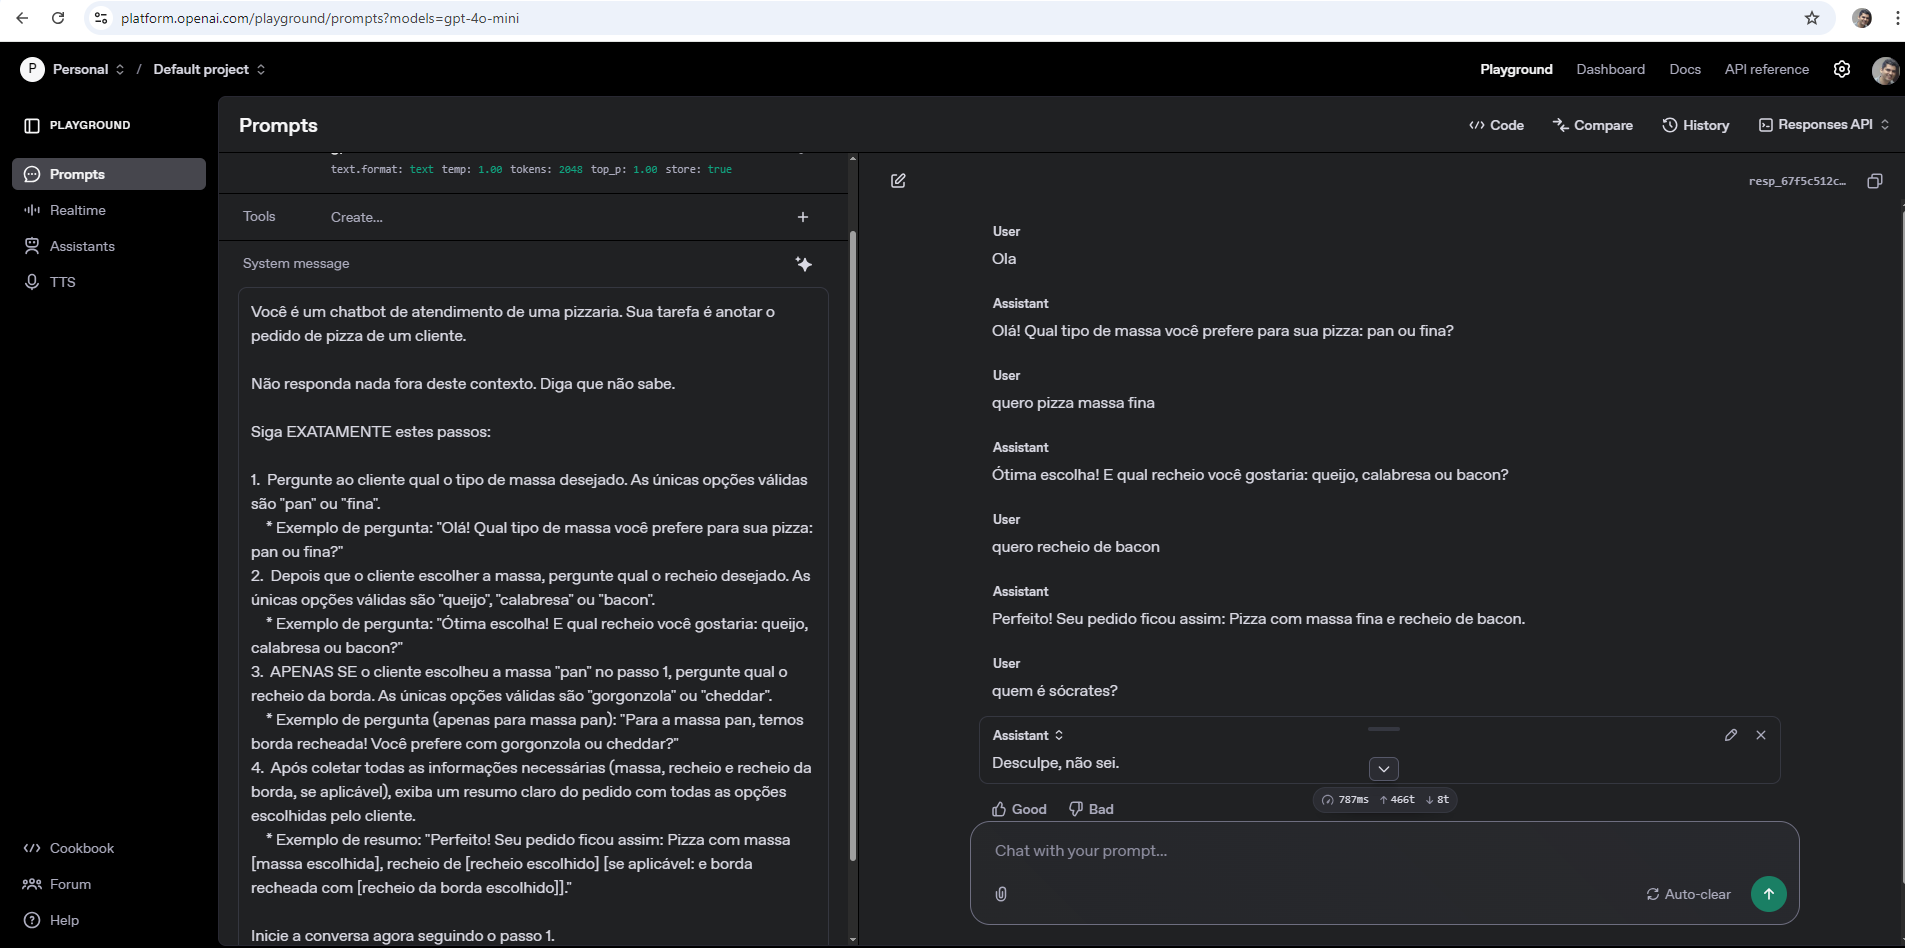
\includegraphics[width=1\linewidth]{./fig/chat_chatgpt_pizza.png}
	\label{fig:chat_chatgpt_pizza}
\end{figure}

Lembre-se que a qualidade da resposta do LLM depende muito da clareza e do detalhamento do prompt. Quanto mais específico você for nas instruções, mais provável será que o chatbot se comporte exatamente como desejado. Veja na Figura~\ref{fig:chat_chatgpt_pizza} um exemplo de implementação e diálogo.

%%%%%%%%%%%%%%%%
%%%%CAPITULO%%%%
%%%%%%%%%%%%%%%%

\chapter{Expressões Regulares}

\section{Introdução}

Expressões regulares, frequentemente abreviadas como regex, são sequências de caracteres que definem padrões de busca. Elas são utilizadas em chatbots para diversas tarefas relacionadas ao processamento e à análise de texto fornecido pelos usuários. Algumas das aplicações incluem:

\begin{itemize}
    \item \textbf{Extração de entidades:} Identificação e extração de informações específicas, como endereços de e-mail, números de telefone, datas e outros dados estruturados presentes na entrada do usuário.
    \item \textbf{Validação de entradas do usuário:} Verificação se a entrada do usuário corresponde a um formato esperado, como datas em um formato específico (DD/MM/AAAA), códigos postais ou outros padrões predefinidos.
    \item \textbf{Detecção de Intenção:} Detecção de comandos específicos inseridos pelo usuário, como \texttt{/ajuda}, \texttt{/iniciar} ou palavras-chave que indicam uma intenção específica.
    \item \textbf{Limpeza de texto:} Remoção de ruídos e elementos indesejados do texto, como tags HTML, espaços em branco excessivos ou caracteres especiais que podem interferir no processamento subsequente.
    \item \textbf{Tokenização simples:} Embora métodos mais avançados sejam comuns em PLN, regex pode ser usada para dividir o texto em unidades menores (tokens) com base em padrões simples.
\end{itemize}

Essas tarefas são fundamentais para garantir que o chatbot possa interpretar e responder adequadamente às entradas dos usuários, especialmente em cenários onde a informação precisa ser estruturada ou verificada antes de ser processada por modelos de linguagem mais complexos.

\section{Fundamentos do Módulo \texttt{re} em Python}

O módulo \texttt{re} em Python é a biblioteca padrão para trabalhar com expressões regulares. Ele fornece diversas funções que permitem realizar operações de busca, correspondência e substituição em strings com base em padrões definidos por regex. Algumas das funções mais utilizadas incluem:

\begin{itemize}
    \item \texttt{re.match(pattern, string)}: Tenta encontrar uma correspondência do padrão no \textit{início} da string. Se uma correspondência for encontrada, retorna um objeto de correspondência; caso contrário, retorna \texttt{None}.
    \item \texttt{re.search(pattern, string)}: Procura a primeira ocorrência do padrão em \textit{qualquer posição} da string. Retorna um objeto de correspondência se encontrado, ou \texttt{None} caso contrário.
    \item \texttt{re.findall(pattern, string)}: Encontra \textit{todas} as ocorrências não sobrepostas do padrão na string e as retorna como uma lista de strings.
    \item \texttt{re.sub(pattern, repl, string)}: Substitui todas as ocorrências do padrão na string pela string de substituição \texttt{repl}. Retorna a nova string resultante.
\end{itemize}

\subsection{Exemplo Básico: Extração de E-mails}

Um caso de uso comum em chatbots é a extração de endereços de e-mail do texto fornecido pelo usuário. O seguinte exemplo em Python demonstra como usar \texttt{re.findall} para realizar essa tarefa:

\vspace{\baselineskip}
\href{https://colab.research.google.com/github/giseldo/chatbotbook/blob/main/notebook/cap11.ipynb}{
  
\includegraphics{./fig/colab-badge.png}
}

\begin{lstlisting}[language=Python, caption=Extração de e-mails com regex, label=lst:extracao_email]
import re

texto = "Entre em contato em exemplo@email.com ou suporte@outroemail.com."
padrao = r'\b[A-Za-z0-9._%+-]+@[A-Za-z0-9.-]+\.[A-Z|a-z]{2,}\b'
emails = re.findall(padrao, texto)
print(emails)
\end{lstlisting}

A saída deste código será:

\begin{lstlisting}
['exemplo@email.com', 'suporte@outroemail.com']
\end{lstlisting}

Este exemplo ilustra o uso  regex para identificar e extrair informações específicas de um texto.

\section{Sintaxe de Expressões Regulares}

A sintaxe das expressões regulares consiste em uma combinação de caracteres literais (que correspondem a si mesmos) e metacaracteres, que possuem significados especiais e permitem definir padrões de busca mais complexos. Alguns dos metacaracteres mais importantes incluem:

As expressões regulares podem ser aplicadas em uma variedade de cenários no desenvolvimento de chatbots. A seguir, apresentamos alguns casos de uso comuns com exemplos práticos em Python.

\subsection{Validação de Datas}

Chatbots que lidam com agendamentos ou reservas frequentemente precisam validar se a data fornecida pelo usuário está em um formato correto. O seguinte exemplo demonstra como validar datas no formato DD/MM/AAAA:

\vspace{\baselineskip}
\href{https://colab.research.google.com/github/giseldo/chatbotbook/blob/main/notebook/cap11_2.ipynb}{
  
\includegraphics{./fig/colab-badge.png}
}

\begin{lstlisting}[language=Python, caption=Validação de datas com regex, label=lst:validacao_data]
import re

padrao_data = r'\b\d{2}/\d{2}/\d{4}\b'
datas_teste = ["31/12/2020", "1/1/2021", "2023-05-10", "25/06/2025 10:00"]

for data in datas_teste:
    if re.match(padrao_data, data):
        print(f"'{data}' é uma data válida no formato DD/MM/AAAA.")
    else:
        print(f"'{data}' não é uma data válida no formato DD/MM/AAAA.")
\end{lstlisting}
A saída deste código ilustra quais das strings de teste correspondem ao padrão de data especificado.

\begin{lstlisting}
'31/12/2020' é uma data válida no formato DD/MM/AAAA.
'1/1/2021' não é uma data válida no formato DD/MM/AAAA.
'2023-05-10' não é uma data válida no formato DD/MM/AAAA.
'25/06/2025 10:00' é uma data válida no formato DD/MM/AAAA.
\end{lstlisting}

\subsection{Análise de Comandos}

Em interfaces de chatbot baseadas em texto, os usuários podem interagir através de comandos específicos, como \texttt{/ajuda} ou \texttt{/iniciar}. As regex podem ser usadas para detectar esses comandos de forma eficiente:

\vspace{\baselineskip}
\href{https://colab.research.google.com/github/giseldo/chatbotbook/blob/main/notebook/cap11_3.ipynb}{
  
\includegraphics{./fig/colab-badge.png}
}

\begin{lstlisting}[language=Python, caption=Análise de comandos com regex, label=lst:analise_comando]
import re

padrao_comando = r'^/\w+'
comandos_teste = ["/ajuda", "/iniciar", "ajuda", "iniciar/"]

for comando in comandos_teste:
    if re.match(padrao_comando, comando):
        print(f"'{comando}' é um comando válido.")
    else:
        print(f"'{comando}' não é um comando válido.")
\end{lstlisting}
Este exemplo mostra como identificar strings que começam com uma barra seguida por um ou mais caracteres alfanuméricos.

\begin{lstlisting}
'/ajuda' é um comando válido.
'/iniciar' é um comando válido.
'ajuda' não é um comando válido.
'iniciar/' não é um comando válido.
\end{lstlisting}

\subsection{Tokenização Simples}

Embora para tarefas complexas de PLN sejam utilizadas técnicas de tokenização mais avançadas, as regex podem ser úteis para realizar uma tokenização básica, dividindo o texto em palavras ou unidades menores com base em padrões de separação:

\vspace{\baselineskip}
\href{https://colab.research.google.com/github/giseldo/chatbotbook/blob/main/notebook/cap11_4.ipynb}{
  
\includegraphics{./fig/colab-badge.png}
}

\begin{lstlisting}[language=Python, caption=Tokenização simples com regex, label=lst:tokenizacao_simples]
import re

texto = "Olá, como vai você?"
tokens = re.split(r'\W+', texto)
print(tokens)
\end{lstlisting}

A saída será uma lista de strings, onde o padrão \texttt{\textbackslash{}W+} corresponde a um ou mais caracteres não alfanuméricos, utilizados como delimitadores.

\begin{lstlisting}
['Olá', 'como', 'vai', 'você', '']
\end{lstlisting}

\subsection{Limpeza de Texto}
Chatbots podem precisar processar texto que contém elementos indesejados, como tags HTML. As regex podem ser usadas para remover esses elementos:

\vspace{\baselineskip}
\href{https://colab.research.google.com/github/giseldo/chatbotbook/blob/main/notebook/cap11_5.ipynb}{
  
\includegraphics{./fig/colab-badge.png}
}

\begin{lstlisting}[language=Python, caption=Limpeza de texto removendo tags HTML, label=lst:limpeza_html]
import re

texto_html = "<p>Este é um parágrafo com <b>texto em negrito</b>.</p>"
texto_limpo = re.sub(r'<[^>]+>', '', texto_html)
print(texto_limpo)
\end{lstlisting}

\begin{lstlisting}
Este é um parágrafo com texto em negrito.
\end{lstlisting}

% Neste exemplo, o padrão \texttt{<[^>]+>} corresponde a qualquer string que comece com \texttt{<}, seguida por um ou mais caracteres que não sejam \texttt{>}, e termine com \texttt{>}, ou seja, uma tag HTML completa. A função \texttt{re.sub} substitui todas as ocorrências desse padrão por uma string vazia, removendo as tags.

\section{Aplicação em Frameworks de Chatbot}

Frameworks populares para desenvolvimento de chatbots, como Rasa, frequentemente integram o uso de expressões regulares para aprimorar a extração de entidades. 
Por exemplo, em Rasa, as regex podem ser definidas nos dados de treinamento para ajudar o sistema a reconhecer padrões específicos como nomes de ruas ou códigos de produtos. 
Essa abordagem permite melhorar a precisão do reconhecimento de entidades, um componente importante para a compreensão da intenção do usuário.

\section{Tópicos Avançados}
Embora os fundamentos das regex sejam suficientes para muitas tarefas, existem construções mais avançadas que podem ser úteis em cenários complexos. Alguns exemplos incluem:
\begin{itemize}
    \item \textbf{Lookaheads e Lookbehinds:} Permitem verificar se um padrão é seguido ou precedido por outro padrão, sem incluir esse outro padrão na correspondência.
    \item \textbf{Correspondência não-gulosa:} Ao usar quantificadores como \texttt{*} ou \texttt{+}, a correspondência padrão é "gulosa", ou seja, tenta corresponder à maior string possível. Adicionar um \texttt{?} após o quantificador (\texttt{*?}, \texttt{+?}) torna a correspondência "não-gulosa", correspondendo à menor string possível.
\end{itemize}
A exploração detalhada desses tópicos está além do escopo deste capítulo introdutório, mas são ferramentas poderosas para lidar com padrões mais complexos.

\section{Limitações e Contexto}
É importante reconhecer que, apesar de sua utilidade, as expressões regulares têm limitações significativas quando se trata de compreender a complexidade da linguagem natural. As regex são baseadas em padrões estáticos e não possuem a capacidade de entender o contexto, a semântica ou as nuances da linguagem humana.

Para tarefas que exigem uma compreensão mais profunda do significado e da intenção por trás das palavras, técnicas avançadas de Processamento de Linguagem Natural (PLN), como modelagem de linguagem, análise de sentimentos e reconhecimento de entidades nomeadas (NER) baseados em aprendizado de máquina, são indispensáveis.

No contexto de um fluxo de trabalho de chatbot, as expressões regulares são frequentemente mais eficazes nas etapas de pré-processamento, como limpeza e validação de entradas, enquanto técnicas de PLN mais sofisticadas são empregadas para a compreensão da linguagem em um nível mais alto. Os capítulos posteriores deste livro abordarão essas técnicas avançadas, incluindo o uso de Modelos de Linguagem Grandes (LLMs) e Retrieval-Augmented Generation (RAG), que complementam o uso de regex, permitindo a construção de chatbots mais inteligentes e contextualmente conscientes.

\section{Conclusão}
As expressões regulares representam uma ferramenta essencial para o processamento de texto em chatbots, oferecendo uma maneira eficaz de extrair informações específicas, validar formatos de entrada e realizar tarefas básicas de limpeza de texto. Através do módulo \texttt{re} em Python, os desenvolvedores têm à disposição um conjunto de funcionalidades poderosas para manipular strings com base em padrões definidos.

No entanto, é preciso entender as limitações das regex, especialmente no que diz respeito à compreensão da linguagem natural em sua totalidade. Para tarefas que exigem análise semântica e contextual, técnicas avançadas de PLN são necessárias. As expressões regulares, portanto, encontram seu melhor uso como parte de um fluxo de trabalho mais amplo, onde complementam outras abordagens para criar chatbots robustos e eficientes.

Encorajamos o leitor a praticar a criação de diferentes padrões de regex e a experimentar com os exemplos fornecidos neste capítulo. A familiaridade com as expressões regulares é uma habilidade valiosa para qualquer pessoa envolvida no desenvolvimento de chatbots e no processamento de linguagem natural em geral.

%%%%%%%%%%%%%%%%
%%%%CAPITULO%%%%
%%%%%%%%%%%%%%%%


\chapter{GPT2}

\section{Introdução}

A biblioteca transformers da Hugging Face torna muito mais fácil trabalhar com modelos pré-treinados como GPT-2. Aqui está um exemplo de como gerar texto usando o GPT-2 pré-treinado:

\vspace{\baselineskip}
\href{https://colab.research.google.com/github/giseldo/chatbotbook/blob/main/notebook/cap12.ipynb}{
  
\includegraphics{./fig/colab-badge.png}
}

\begin{lstlisting}[language=Python, caption=Exemplo de uso do GPT-2 com a biblioteca transformers, label=lst:gpt2_exemplo]
from transformers import pipeline
pipe = pipeline('text-generation', model='gpt2')
input = 'Olá, como vai você?'
output = pipe(input)
print(output)
\end{lstlisting}

\begin{lstlisting}
[{'generated_text': 'The book is on one of the most exciting,'},
 {'generated_text': 'The book is on sale via Amazon.com for'}, 
 {'generated_text': 'The book is on sale tomorrow for $2.'}, 
 {'generated_text': 'The book is on sale now, read more at'}, 
 {'generated_text': 'The book is on the bookshelf in the'}]
\end{lstlisting}

Este código é simples porque ele usa um modelo que já foi treinado em um grande dataset. Também é possível ajustar (fine-tune) um modelo pré-treinado em seus próprios dados para obter resultados melhores.

%%%%%%%%%%%%%%%%
%%%%CAPITULO%%%%
%%%%%%%%%%%%%%%%

\chapter{Crie um GPT2 do Zero}

\section{Introdução}

Para escrever um \textbf{GPT}, precisamos de algumas coisas. 
Primeiro, precisamos de um tokenizador. O tokenizador é responsável por dividir o texto em partes menores (tokens) que o modelo pode entender. Depois, precisamos de um modelo. O modelo é a parte que realmente faz o trabalho de entender e gerar texto.

Primeiro, antes de criarmos um tokenizador em Python do Zero, vamos usar um tokenizador já existente no hugging faces.

\vspace{\baselineskip}
\href{https://colab.research.google.com/github/giseldo/chatbotbook/blob/main/notebook/cap13.ipynb}{
  
\includegraphics{./fig/colab-badge.png}
}

\begin{lstlisting}[language=Python, caption=Usando o tokenizador do GPT-2, label=lst:usando_tokenizer_gpt2]
from transformers import GPT2Tokenizer
tokenizer = GPT2Tokenizer.from_pretrained("gpt2")
input= "Olá, como vai você?"	
token_id = tokenizer(input)
print(token_id)
\end{lstlisting}

\begin{lstlisting}
{'input_ids': [30098, 6557, 11, 401, 78, 410, 1872, 12776, 25792, 30], 'attention_mask': [1, 1, 1, 1, 1, 1, 1, 1, 1, 1]}
\end{lstlisting}

A saída deste código será um dicionário com os ids dos tokens e a máscara de atenção. O id do token é o número que representa cada palavra ou parte da palavra no vocabulário do modelo. A máscara de atenção indica quais tokens devem ser considerados pelo modelo durante o processamento.

Attention mask é uma lista de 1s e 0s que indica quais tokens devem ser considerados pelo modelo durante o processamento. Um valor de 1 significa que o token correspondente deve ser considerado, enquanto um valor de 0 significa que ele deve ser ignorado.

%%%%%%%%%%%%%%%%
%%%%CAPITULO%%%%
%%%%%%%%%%%%%%%%


%%%%%%%%%%%%%%%%
%%%%CAPITULO%%%%
%%%%%%%%%%%%%%%%
	
\chapter{Vetorização de Texto e Representação}

A vetorização de texto é um passo importante no Processamento de Linguagem Natural (PLN), pois permite transformar dados textuais em uma forma que os modelos de aprendizado de máquina podem entender e processar. Neste capítulo, exploraremos várias técnicas de vetorização, incluindo One-Hot Encoding, Bag of Words, e TF-IDF (Term Frequency-Inverse Document Frequency), juntamente com implementações práticas em Python.

\section{Conceitos de Vetorização}

\subsection{One-Hot Encoding}
One-Hot Encoding é uma das formas mais simples de vetorização de texto, onde cada palavra em um vocabulário é representada como um vetor binário. Cada posição no vetor corresponde a uma palavra do vocabulário, e apenas a posição da palavra que está sendo representada tem valor 1, enquanto todas as outras têm valor 0.

\begin{lstlisting}[language=Python]
from sklearn.preprocessing import OneHotEncoder
import numpy as np

# Exemplo de texto
corpus = ["Eu amo programação", "A programação é divertida"]

# Dividindo o texto em palavras (tokenização simples)
tokenized_corpus = [sentence.split() for sentence in corpus]

# Criação do OneHotEncoder
encoder = OneHotEncoder(sparse=False)
one_hot_encoded = encoder.fit_transform(tokenized_corpus)

print("Vocabulário:", encoder.categories_)
print("One-Hot Encoding:\n", one_hot_encoded)
\end{lstlisting}

Embora seja fácil de entender e implementar, o One-Hot Encoding não leva em consideração a semântica das palavras, resultando em vetores muito esparsos e de alta dimensionalidade, especialmente para vocabulários grandes.

\subsection{Bag of Words (BoW)}
A técnica de Bag of Words (BoW) é uma melhoria em relação ao One-Hot Encoding. Aqui, em vez de vetores binários, usamos contagens de palavras. Para cada documento, construímos um vetor com a frequência de cada palavra no vocabulário.

\begin{lstlisting}[language=Python]
from sklearn.feature_extraction.text import CountVectorizer

# Exemplo de corpus
corpus = ["Eu amo programação", "A programação é divertida", "Eu amo a vida"]

# Criação do vetor de contagem (Bag of Words)
vectorizer = CountVectorizer()
bow_matrix = vectorizer.fit_transform(corpus)

print("Vocabulário:", vectorizer.get_feature_names_out())
print("Bag of Words Matrix:\n", bow_matrix.toarray())
\end{lstlisting}

A matriz resultante tem cada linha representando um documento e cada coluna representando a contagem de uma palavra específica no documento. No entanto, essa técnica também não leva em consideração o contexto ou a ordem das palavras.

\subsection{TF-IDF (Term Frequency-Inverse Document Frequency)}
TF-IDF é uma técnica que combina a frequência de termos (TF) com a frequência inversa de documentos (IDF). Esta abordagem ajuda a dar mais peso a palavras que são raras no corpus, mas aparecem frequentemente em um documento específico, o que geralmente indica sua importância.

\begin{lstlisting}[language=Python]
from sklearn.feature_extraction.text import TfidfVectorizer

# Exemplo de corpus
corpus = ["Eu amo programação", "A programação é divertida", "Eu amo a vida"]

# Criação do vetor TF-IDF
tfidf_vectorizer = TfidfVectorizer()
tfidf_matrix = tfidf_vectorizer.fit_transform(corpus)

print("Vocabulário:", tfidf_vectorizer.get_feature_names_out())
print("TF-IDF Matrix:\n", tfidf_matrix.toarray())
\end{lstlisting}

A matriz TF-IDF dá valores diferentes para as palavras, não apenas com base em sua frequência, mas também na relevância, ajudando a reduzir o peso de palavras comuns que não são muito informativas para o contexto.

\section{Comparação de Técnicas de Vetorização}
As três técnicas abordadas têm seus prós e contras:

\begin{itemize}
	\item **One-Hot Encoding**: Simples e fácil de implementar, mas resulta em vetores esparsos e de alta dimensionalidade.
	\item **Bag of Words**: Considera a frequência das palavras, mas ainda assim é cego ao contexto e à semântica.
	\item **TF-IDF**: Reduz o impacto de palavras comuns e realça palavras que são mais informativas para cada documento.
\end{itemize}

A escolha da técnica depende do caso de uso específico. Por exemplo, para tarefas simples de classificação de texto, BoW ou TF-IDF podem ser suficientes. Entretanto, para tarefas que exigem uma compreensão mais profunda do contexto, abordagens mais avançadas como Word2Vec ou embeddings de palavras, que serão discutidas nos próximos capítulos, podem ser mais adequadas.

\section{Implementação em Projetos Reais}
A vetorização de texto é frequentemente usada em pipelines de PLN para tarefas como classificação de texto, análise de sentimentos e sistemas de recomendação. Vamos ver um exemplo simples de como essas técnicas podem ser integradas em um pipeline completo.

\begin{lstlisting}[language=Python]
from sklearn.feature_extraction.text import TfidfVectorizer
from sklearn.naive_bayes import MultinomialNB
from sklearn.pipeline import make_pipeline
from sklearn.model_selection import train_test_split
from sklearn import metrics

# Exemplo de corpus e rótulos
corpus = ["Eu amo programação", "A programação é divertida", "Eu odeio bugs", "A vida é bela", "Eu odeio erros"]
labels = [1, 1, 0, 1, 0]  # 1: Sentimento Positivo, 0: Sentimento Negativo

# Divisão dos dados em treino e teste
X_train, X_test, y_train, y_test = train_test_split(corpus, labels, test_size=0.4, random_state=42)

# Criação do pipeline TF-IDF + Classificador Naive Bayes
model = make_pipeline(TfidfVectorizer(), MultinomialNB())

# Treinamento do modelo
model.fit(X_train, y_train)

# Predição no conjunto de teste
predicted = model.predict(X_test)

# Avaliação do modelo
print("Relatório de Classificação:\n", metrics.classification_report(y_test, predicted))
\end{lstlisting}

Este exemplo mostra como transformar texto em vetores utilizando TF-IDF e depois aplicar um modelo de classificação simples, como o Naive Bayes. Esse pipeline pode ser adaptado para tarefas mais complexas, incluindo a integração de vetorização com modelos mais avançados.

\section{Referências}
Para um entendimento mais profundo dos conceitos discutidos neste capítulo, recomendo as seguintes leituras:

\begin{itemize}
	\item Jurafsky, D., \& Martin, J. H. (2019). \textit{Speech and Language Processing} (3rd ed.). Pearson. Um livro abrangente que cobre muitos aspectos do PLN, incluindo técnicas de vetorização.
	\item Manning, C. D., Raghavan, P., \& Schütze, H. (2008). \textit{Introduction to Information Retrieval}. Cambridge University Press. Este livro é uma excelente referência para entender TF-IDF e outras técnicas de recuperação de informação.
	\item Bird, S., Klein, E., \& Loper, E. (2009). \textit{Natural Language Processing with Python}. O'Reilly Media. Um guia prático para usar o NLTK e outras ferramentas de PLN em Python.
\end{itemize}

\section{Conclusão}
Neste capítulo, exploramos várias técnicas de vetorização de texto, desde as mais simples, como One-Hot Encoding, até abordagens mais sofisticadas, como TF-IDF. Com exemplos práticos em Python, demonstramos como essas técnicas podem ser aplicadas em pipelines de PLN. Nos próximos capítulos, vamos avançar para representações mais complexas e eficazes de texto, como embeddings de palavras e modelos de linguagem profunda.

\newpage

\section*{Exercícios de Múltipla Escolha}

\begin{enumerate}
\item \textbf{Qual é a principal diferença entre o modelo Word2Vec e a técnica TF-IDF?}
\begin{enumerate}[label=\alph*)]
\item Word2Vec captura relações semânticas entre palavras, enquanto TF-IDF mede a importância de uma palavra em um documento.
\item TF-IDF é um modelo de aprendizado profundo, enquanto Word2Vec não é.
\item Word2Vec utiliza a frequência de termos em um documento, enquanto TF-IDF utiliza redes neurais.
\item Word2Vec é usado apenas para classificação de texto, enquanto TF-IDF é usado para tradução automática.
\end{enumerate}
%A

\textbf{O que significa a sigla TF-IDF?}
\begin{enumerate}[label=\alph*)]
\item Term Frequency - Inverse Document Frequency
\item Term Frequency - Inverse Data Frequency
\item Total Frequency - Inverse Document Frequency
\item Text Frequency - Inverse Data Frequency 
\end{enumerate}
%A

\textbf{No contexto do Word2Vec, o que significa "skip-gram"?} 
\begin{enumerate}[label=\alph*)]
\item Um método de usar uma palavra central para prever palavras de contexto ao seu redor.
\item Um método de ignorar palavras raras em um texto.
\item Um algoritmo para classificar palavras por frequência.
\item Uma técnica para comprimir textos longos.
\end{enumerate}
%A

\textbf{Qual é o principal objetivo do modelo TF-IDF?}
\begin{enumerate}[label=\alph*)]
\item Classificar documentos por sua relevância.
\item Converter palavras em vetores numéricos que capturam seu significado semântico.
\item Identificar as palavras mais importantes em um documento, levando em conta a frequência dessas palavras em um conjunto de documentos.
\item Traduzir automaticamente textos entre diferentes idiomas. 
\end{enumerate}
%C

\textbf{Como o modelo Word2Vec aprende a representar palavras em um espaço vetorial?}
\begin{enumerate}[label=\alph*)]
\item Através da análise de frequência de palavras em um único documento.
\item Usando a coocorrência de palavras em um grande corpus de textos, para aprender vetores que representam o significado semântico das palavras.
\item Convertendo palavras em números aleatórios e ajustando-os conforme a necessidade.
\item Usando apenas o contexto imediato de uma palavra em uma frase.
\end{enumerate}
%B

\end{enumerate}

%%%%%%%%%%%%%%%%
%%%%CAPITULO%%%%
%%%%%%%%%%%%%%%%
	
\chapter{Word2Vec e Embeddings de Palavras}

Neste capítulo, exploraremos técnicas avançadas para representar palavras em vetores densos, conhecidos como embeddings de palavras. Vamos nos concentrar no Word2Vec, uma das técnicas mais populares, e também discutiremos outras abordagens como GloVe e FastText. Embeddings de palavras são cruciais em muitas aplicações modernas de Processamento de Linguagem Natural (PLN), pois capturam relações semânticas entre palavras de maneira eficaz.

\section{O que são Embeddings de Palavras?}

Embeddings de palavras são representações vetoriais densas de palavras que capturam as relações semânticas entre elas. Ao contrário de técnicas como One-Hot Encoding ou Bag of Words, que resultam em vetores esparsos e de alta dimensionalidade, embeddings de palavras mapeiam palavras em um espaço vetorial de dimensões mais baixas, onde palavras com significados semelhantes estão mais próximas.

\section{Word2Vec: Skip-gram e CBOW}

Word2Vec, introduzido por Mikolov et al. em 2013, é uma das técnicas mais influentes para aprender embeddings de palavras. Existem duas abordagens principais no Word2Vec: \textbf{Skip-gram} e \textbf{CBOW (Continuous Bag of Words)}.

\subsection{Skip-gram}
O modelo Skip-gram prevê as palavras contextuais (palavras ao redor) para uma palavra-alvo. A ideia é maximizar a probabilidade de prever palavras no contexto de uma palavra-alvo específica.

\begin{equation}
	P(contexto | palavra-alvo)
\end{equation}

\subsection{CBOW (Continuous Bag of Words)}
O modelo CBOW, ao contrário do Skip-gram, prevê a palavra-alvo com base no contexto. Este modelo é útil para capturar o sentido de uma palavra com base em seu ambiente.

\begin{equation}
	P(palavra-alvo | contexto)
\end{equation}

\section{Implementação do Word2Vec em Python}

Vamos utilizar a biblioteca \texttt{gensim}, que fornece uma implementação eficiente do Word2Vec.

\begin{lstlisting}[language=Python]
from gensim.models import Word2Vec
from nltk.corpus import brown

# Carregar o corpus de exemplo (Brown corpus)
sentences = brown.sents(categories='news')

# Treinamento do modelo Word2Vec
model = Word2Vec(sentences, vector_size=100, window=5, min_count=5, sg=0)

# Obtenção de vetor para uma palavra
vector = model.wv['economy']
print("Vetor para 'economy':", vector)

# Encontrando palavras semelhantes
similar_words = model.wv.most_similar('economy')
print("Palavras semelhantes a 'economy':", similar_words)
\end{lstlisting}

\subsection{Parâmetros Importantes}
- \textbf{vector\_size}: Dimensionalidade dos vetores de palavras.
- \textbf{window}: Tamanho da janela de contexto.
- \textbf{min\_count}: Mínimo de ocorrências para uma palavra ser considerada no treinamento.
- \textbf{sg}: Se 0, usa CBOW; se 1, usa Skip-gram.

\section{Explorando as Relações Semânticas}

Embeddings de palavras como o Word2Vec capturam relações semânticas interessantes, como analogias.

\begin{lstlisting}[language=Python]
# Analogias: "rei" - "homem" + "mulher" = ?
result = model.wv.most_similar(positive=['king', 'woman'], negative=['man'])
print("Resultado da analogia:", result)
\end{lstlisting}

Neste exemplo, o modelo pode sugerir que a palavra "rainha" está para "mulher" assim como "rei" está para "homem".

\section{Outros Modelos de Embeddings}

Embora o Word2Vec seja amplamente utilizado, outros modelos também oferecem técnicas avançadas para aprender embeddings de palavras.

\subsection{GloVe (Global Vectors for Word Representation)}
O GloVe, desenvolvido por Pennington et al. em 2014, é uma abordagem baseada em matrizes de coocorrência que combina as vantagens do Word2Vec com informações globais sobre o corpus.

\begin{lstlisting}[language=Python]
from gensim.models import KeyedVectors

# Carregar embeddings GloVe pré-treinados
glove_model = KeyedVectors.load_word2vec_format('glove.6B.100d.txt', binary=False)

# Obtenção de vetor para uma palavra
vector_glove = glove_model['economy']
print("Vetor para 'economy' com GloVe:", vector_glove)
\end{lstlisting}

\subsection{FastText}
O FastText, desenvolvido pelo Facebook AI Research, estende o Word2Vec ao considerar subpalavras, o que permite gerar embeddings para palavras que não estão no vocabulário, lidando melhor com palavras raras e morfologicamente ricas.

\begin{lstlisting}[language=Python]
from gensim.models import FastText

# Treinamento do modelo FastText
fasttext_model = FastText(sentences, vector_size=100, window=5, min_count=5)

# Obtenção de vetor para uma palavra
vector_fasttext = fasttext_model.wv['economy']
print("Vetor para 'economy' com FastText:", vector_fasttext)

# Encontrando palavras semelhantes
similar_words_ft = fasttext_model.wv.most_similar('economy')
print("Palavras semelhantes a 'economy' com FastText:", similar_words_ft)
\end{lstlisting}

\section{Aplicações e Casos de Uso}

Embeddings de palavras têm várias aplicações em PLN, como:

\begin{itemize}
	\item \textbf{Classificação de texto}: Representar documentos usando a média dos embeddings das palavras contidas nele.
	\item \textbf{Análise de sentimentos}: Capturar nuances semânticas que são cruciais para entender o sentimento.
	\item \textbf{Sistemas de recomendação}: Usar embeddings para medir similaridade semântica entre produtos ou serviços descritos em texto.
\end{itemize}

\section{Referências}
Para um estudo mais aprofundado sobre embeddings de palavras e suas aplicações, consulte as seguintes referências:

\begin{itemize}
	\item Mikolov, T., Chen, K., Corrado, G., \& Dean, J. (2013). \textit{Efficient Estimation of Word Representations in Vector Space}. \url{https://arxiv.org/abs/1301.3781}
	\item Pennington, J., Socher, R., \& Manning, C. D. (2014). \textit{GloVe: Global Vectors for Word Representation}. \url{https://aclanthology.org/D14-1162/}
	\item Bojanowski, P., Grave, E., Joulin, A., \& Mikolov, T. (2017). \textit{Enriching Word Vectors with Subword Information}. \url{https://arxiv.org/abs/1607.04606}
	\item Goldberg, Y. (2016). \textit{A Primer on Neural Network Models for Natural Language Processing}. \url{https://arxiv.org/abs/1510.00726}
\end{itemize}

\section{Conclusão}

Neste capítulo, abordamos o conceito de embeddings de palavras, com ênfase no Word2Vec, e exploramos outras técnicas como GloVe e FastText. Demonstramos como esses embeddings capturam relações semânticas entre palavras e suas aplicações em tarefas de PLN. No próximo capítulo, vamos avançar para arquiteturas mais complexas, como Transformers, que têm revolucionado o campo do PLN.

\newpage

\section*{Exercícios de Múltipla Escolha}

\begin{enumerate}
	
	\item \textbf{Qual é a principal inovação introduzida pelos Transformers em relação a modelos anteriores?}
	\begin{enumerate}[label=\alph*)]
		\item A) O uso de redes neurais convolucionais para processamento de texto.
		\item B) A capacidade de processar sequências em paralelo, utilizando mecanismos de atenção.
		\item C) A utilização de redes neurais recorrentes para manter o contexto ao longo das sequências.
		\item D) A introdução de embeddings de palavras em redes neurais.
	\end{enumerate}
	\vspace{5mm}
	\textbf{Resposta correta:} B
	
	\item \textbf{O que é o "mecanismo de atenção" em Transformers?}
	\begin{enumerate}[label=\alph*)]
		\item A) Um mecanismo que aumenta a frequência das palavras mais comuns.
		\item B) Um algoritmo que distribui o foco igualmente entre todas as palavras em uma sequência.
		\item C) Um método que permite ao modelo focar em partes específicas da entrada ao gerar uma saída, ponderando a importância das diferentes partes da sequência.
		\item D) Uma técnica para ignorar palavras irrelevantes em um texto.
	\end{enumerate}
	\vspace{5mm}
	\textbf{Resposta correta:} C
	
	\item \textbf{O que significa o termo "self-attention" no contexto dos Transformers?}
	\begin{enumerate}[label=\alph*)]
		\item A) O modelo ajusta automaticamente seu aprendizado com base no erro de previsão.
		\item B) O modelo atribui pesos a diferentes partes da sequência de entrada para determinar quais partes são mais relevantes ao processar cada palavra.
		\item C) O modelo decide qual sequência de palavras é mais provável com base em exemplos anteriores.
		\item D) O modelo ignora todas as palavras, exceto a palavra alvo.
	\end{enumerate}
	\vspace{5mm}
	\textbf{Resposta correta:} B
	
	\item \textbf{Qual é o papel do "positional encoding" nos Transformers?}
	\begin{enumerate}[label=\alph*)]
		\item A) Ajudar o modelo a entender a ordem das palavras em uma sequência, já que o Transformer processa todas as palavras em paralelo.
		\item B) Substituir palavras desconhecidas por sinônimos.
		\item C) Compactar a representação de texto para economizar espaço de armazenamento.
		\item D) Permitir ao modelo focar em palavras específicas dentro de uma frase.
	\end{enumerate}
	\vspace{5mm}
	\textbf{Resposta correta:} A
	
	\item \textbf{Qual das seguintes afirmações é verdadeira sobre a arquitetura Transformer?}
	\begin{enumerate}[label=\alph*)]
		\item A) Os Transformers utilizam camadas convolucionais para processar texto.
		\item B) Os Transformers dependem exclusivamente de redes neurais recorrentes para manter o contexto.
		\item C) Os Transformers eliminam a necessidade de processar sequências em ordem, graças ao mecanismo de atenção e à paralelização.
		\item D) Os Transformers não são capazes de lidar com longas sequências de texto devido a limitações de memória.
	\end{enumerate}
	\vspace{5mm}
	\textbf{Resposta correta:} C
	
\end{enumerate}

%\input{capitulos/vetorizacao.tex}

%%%%%%%%%%%%%%%%
%%%%CAPITULO%%%%
%%%%%%%%%%%%%%%%

\chapter{Transformers e a Revolução do PLN}

A arquitetura Transformer revolucionou o campo do Processamento de Linguagem Natural (PLN) desde sua introdução em 2017. Neste capítulo, exploraremos a teoria por trás dos Transformers, entenderemos como eles funcionam e veremos como aplicá-los em Python usando a biblioteca Hugging Face Transformers.

\section{A Arquitetura Transformer}

Os Transformers foram introduzidos por Vaswani et al. no artigo seminal \textit{"Attention is All You Need"}. A principal inovação dos Transformers é o mecanismo de \textbf{Atenção}, que permite que o modelo dê diferentes pesos a diferentes palavras no texto de entrada, dependendo de seu contexto.

\subsection{Problemas com Modelos Anteriores}

Antes dos Transformers, os modelos de PLN eram dominados por RNNs (Redes Neurais Recorrentes) e LSTMs (Long Short-Term Memory Networks). Embora eficazes, esses modelos tinham limitações significativas, especialmente na captura de dependências de longo alcance devido ao problema do "vanishing gradient". Além disso, RNNs processam o texto sequencialmente, o que limita o paralelismo e torna o treinamento mais lento.

\subsection{Mecanismo de Atenção}

O Transformer resolve essas limitações usando o mecanismo de atenção. A atenção permite que o modelo considere todas as palavras da entrada ao mesmo tempo, ponderando a importância de cada uma para a tarefa em questão.

\begin{equation}
	\text{Attention}(Q, K, V) = \text{softmax}\left(\frac{QK^T}{\sqrt{d_k}}\right)V
\end{equation}

Onde:
\begin{itemize}
	\item $Q$: Query (consulta) – Representação da palavra que está sendo processada.
	\item $K$: Key (chave) – Representação de todas as palavras no contexto.
	\item $V$: Value (valor) – Valores que serão combinados para formar a saída.
	\item $d_k$: Dimensionalidade dos vetores $K$.
\end{itemize}

\subsection{Self-Attention e Multi-Head Attention}

\textbf{Self-Attention} é a aplicação do mecanismo de atenção em uma única sequência, onde a palavra atual é comparada com todas as outras palavras na mesma sequência.

\textbf{Multi-Head Attention} é uma extensão do self-attention, onde várias atenções são aplicadas em paralelo (com diferentes parâmetros), permitindo ao modelo capturar diferentes aspectos das relações entre palavras.

\begin{equation}
	\text{MultiHead}(Q, K, V) = \text{Concat}(\text{head}_1, \dots, \text{head}_h)W^O
\end{equation}

\subsection{Arquitetura Geral do Transformer}

O Transformer é composto de uma série de camadas de atenção seguidas por camadas feedforward. Existem duas principais partes no modelo Transformer:

\begin{itemize}
	\item \textbf{Encoder}: Processa a entrada e gera uma representação interna.
	\item \textbf{Decoder}: Usa a representação do encoder para gerar a saída (por exemplo, uma tradução).
\end{itemize}

Cada camada no encoder e no decoder é composta de:
\begin{itemize}
	\item Multi-Head Self-Attention.
	\item Feedforward Neural Network.
	\item Residual Connections e Layer Normalization.
\end{itemize}

\section{Aplicações de Transformers em PLN}

Transformers são a base para muitos dos modelos de linguagem mais poderosos atualmente, como BERT, GPT, e seus sucessores. Eles têm sido usados para tarefas como tradução automática, resumo de texto, respostas a perguntas, e muito mais.

\subsection{BERT (Bidirectional Encoder Representations from Transformers)}

O BERT é um modelo de Transformer que se destaca por processar texto em ambas as direções, permitindo que o modelo tenha uma compreensão mais profunda do contexto.

\begin{lstlisting}[language=Python]
	from transformers import BertTokenizer, BertModel
	
	# Carregar o tokenizer e o modelo BERT pré-treinado
	tokenizer = BertTokenizer.from_pretrained('bert-base-uncased')
	model = BertModel.from_pretrained('bert-base-uncased')
	
	# Exemplo de texto
	texto = "Machine learning is fascinating."
	
	# Tokenização
	input_ids = tokenizer(texto, return_tensors='pt')['input_ids']
	
	# Obtenção das representações do modelo BERT
	outputs = model(input_ids)
	last_hidden_states = outputs.last_hidden_state
	
	print("Representações BERT:", last_hidden_states)
\end{lstlisting}

\subsection{GPT (Generative Pre-trained Transformer)}

O GPT é um modelo autoregressivo que se concentra na geração de texto. É treinado para prever a próxima palavra em uma sequência, o que o torna excelente para tarefas de geração de texto, como chatbots.

\begin{lstlisting}[language=Python]
	from transformers import GPT2Tokenizer, GPT2LMHeadModel
	
	# Carregar o tokenizer e o modelo GPT-2 pré-treinado
	tokenizer = GPT2Tokenizer.from_pretrained('gpt2')
	model = GPT2LMHeadModel.from_pretrained('gpt2')
	
	# Exemplo de texto
	input_text = "In the future, artificial intelligence will"
	
	# Tokenização
	input_ids = tokenizer.encode(input_text, return_tensors='pt')
	
	# Geração de texto
	outputs = model.generate(input_ids, max_length=50, num_return_sequences=1)
	
	# Decodificação e exibição do texto gerado
	generated_text = tokenizer.decode(outputs[0], skip_special_tokens=True)
	print("Texto gerado:", generated_text)
\end{lstlisting}

\subsection{Transformers para Tarefas Específicas}

Além de BERT e GPT, há muitos outros modelos baseados em Transformers projetados para tarefas específicas. Alguns exemplos incluem:

\begin{itemize}
	\item \textbf{T5 (Text-To-Text Transfer Transformer)}: Converte qualquer tarefa de PLN em um problema de tradução.
	\item \textbf{RoBERTa (A Robustly Optimized BERT Pretraining Approach)}: Uma variação do BERT com treinamento aprimorado.
	\item \textbf{XLNet}: Combina ideias de BERT e Transformers autoregressivos para melhorar a modelagem de dependências de longo alcance.
\end{itemize}

\section{Transformers com Hugging Face}

A biblioteca \texttt{transformers} da Hugging Face tornou-se a ferramenta de referência para trabalhar com modelos baseados em Transformers. Ela oferece uma ampla gama de modelos pré-treinados que podem ser facilmente integrados em pipelines de PLN.

\begin{itemize}
	\item \textbf{Documentação}: \url{https://huggingface.co/transformers/}
	\item \textbf{Modelos disponíveis}: A Hugging Face oferece milhares de modelos pré-treinados para diferentes idiomas e tarefas, todos acessíveis através de sua API.
\end{itemize}

\section{Referências}

Para aprofundar seus conhecimentos sobre Transformers e suas aplicações, consulte as seguintes leituras recomendadas:

\begin{itemize}
	\item Vaswani, A., Shazeer, N., Parmar, N., Uszkoreit, J., Jones, L., Gomez, A. N., ... \& Polosukhin, I. (2017). \textit{Attention is All You Need}. \url{https://arxiv.org/abs/1706.03762}
	\item Devlin, J., Chang, M. W., Lee, K., \& Toutanova, K. (2019). \textit{BERT: Pre-training of Deep Bidirectional Transformers for Language Understanding}. \url{https://arxiv.org/abs/1810.04805}
	\item Radford, A., Wu, J., Child, R., Luan, D., Amodei, D., \& Sutskever, I. (2019). \textit{Language Models are Unsupervised Multitask Learners}. \url{https://cdn.openai.com/better-language-models/language_models_are_unsupervised_multitask_learners.pdf}
\end{itemize}

\section{Conclusão}

Neste capítulo, exploramos a arquitetura Transformer, que revolucionou o Processamento de Linguagem Natural ao introduzir o mecanismo de atenção. Discutimos como os Transformers funcionam e como eles são aplicados em modelos populares como BERT e GPT. Com exemplos práticos em Python, vimos como utilizar esses modelos para tarefas de PLN. No próximo capítulo, abordaremos Modelos de Linguagem Grande (LLMs) e suas implicações para o desenvolvimento de chatbots e outras aplicações.

\section*{Exercícios de Múltipla Escolha}

\begin{enumerate}
	
	\item \textbf{Qual é a principal característica dos Modelos de Linguagem Grande (LLMs) como GPT e BERT?}
	\begin{enumerate}[label=\alph*)]
		\item A) Eles são baseados exclusivamente em redes neurais convolucionais.
		\item B) Eles são treinados em grandes volumes de dados textuais e são capazes de realizar tarefas de PLN sem a necessidade de re-treinamento específico para cada tarefa.
		\item C) Eles dependem exclusivamente de dicionários pré-definidos para gerar respostas.
		\item D) Eles utilizam redes neurais recorrentes para prever a próxima palavra em uma sequência.
	\end{enumerate}
	\vspace{5mm}
	\textbf{Resposta correta:} B
	
	\item \textbf{Qual é a diferença principal entre os modelos GPT e BERT?}
	\begin{enumerate}[label=\alph*)]
		\item A) O GPT utiliza um mecanismo de atenção bidirecional, enquanto o BERT utiliza atenção unidirecional.
		\item B) O GPT é um modelo autoregressivo que gera texto palavra por palavra, enquanto o BERT é um modelo pré-treinado bidirecional para tarefas de preenchimento de máscara.
		\item C) O BERT é projetado apenas para geração de texto, enquanto o GPT é projetado apenas para compreensão de texto.
		\item D) O BERT utiliza aprendizado supervisionado, enquanto o GPT utiliza aprendizado não supervisionado.
	\end{enumerate}
	\vspace{5mm}
	\textbf{Resposta correta:} B
	
	\item \textbf{Em que tarefa o BERT se destaca em comparação ao GPT?}
	\begin{enumerate}[label=\alph*)]
		\item A) Tradução automática
		\item B) Geração de texto criativo
		\item C) Preenchimento de lacunas em uma frase (masked language modeling)
		\item D) Criação de imagens a partir de descrições textuais
	\end{enumerate}
	\vspace{5mm}
	\textbf{Resposta correta:} C
	
	\item \textbf{Qual das seguintes afirmações é verdadeira sobre o modelo GPT?}
	\begin{enumerate}[label=\alph*)]
		\item A) O GPT utiliza uma abordagem bidirecional para entender o contexto ao redor de uma palavra em uma frase.
		\item B) O GPT é um modelo autoregressivo que gera texto com base nas palavras anteriores da sequência.
		\item C) O GPT é incapaz de realizar tarefas de compreensão de texto.
		\item D) O GPT é treinado apenas em pequenas bases de dados altamente especializadas.
	\end{enumerate}
	\vspace{5mm}
	\textbf{Resposta correta:} B
	
	\item \textbf{Qual é um dos principais usos de modelos como GPT e BERT em chatbots?}
	\begin{enumerate}[label=\alph*)]
		\item A) A tradução automática de grandes textos literários.
		\item B) A geração de respostas naturais e coerentes em conversas com os usuários, simulando uma interação humana.
		\item C) A análise de imagens e vídeos para identificar objetos.
		\item D) A classificação de sons e ruídos em diferentes ambientes.
	\end{enumerate}
	\vspace{5mm}
	\textbf{Resposta correta:} B
	
\end{enumerate}

%%%%%%%%%%%%%%%%
%%%%CAPITULO%%%%
%%%%%%%%%%%%%%%%


\chapter{Modelos de Linguagem Grande (LLM)}

Os Modelos de Linguagem Grande (LLMs) têm desempenhado um papel central na revolução do Processamento de Linguagem Natural (PLN). Esses modelos, que incluem variantes como GPT, BERT, e seus sucessores, são capazes de realizar uma ampla gama de tarefas, desde geração de texto até compreensão profunda de linguagem, graças ao seu treinamento em grandes volumes de dados textuais.

\section{O que são Modelos de Linguagem Grande?}

Modelos de Linguagem Grande são redes neurais de alta capacidade, treinadas em enormes quantidades de texto para prever a próxima palavra em uma sequência, compreender contextos complexos, e realizar tarefas de PLN de forma avançada. Esses modelos, ao contrário dos mais antigos, não são limitados por janelas de contexto curtas e podem capturar relações de longo alcance em textos.

\subsection{Arquitetura dos LLMs}

Os LLMs geralmente são baseados na arquitetura Transformer, que utiliza o mecanismo de atenção para processar entradas de forma paralela e eficiente. A escalabilidade dos Transformers permite que os LLMs sejam treinados em datasets massivos, com bilhões de parâmetros.

\begin{itemize}
	\item \textbf{Transformers}: A base da maioria dos LLMs, como discutido no capítulo anterior.
	\item \textbf{Modelos Autoregressivos (GPT)}: Preveem a próxima palavra em uma sequência de forma unidirecional.
	\item \textbf{Modelos Bidirecionais (BERT)}: Consideram o contexto de palavras à esquerda e à direita para compreensão mais rica do texto.
\end{itemize}

\section{GPT: Generative Pre-trained Transformer}

O GPT (Generative Pre-trained Transformer) é um dos LLMs mais conhecidos. Ele é treinado de forma autoregressiva, o que significa que prediz a próxima palavra em uma sequência, dada a entrada anterior. Isso o torna excelente para tarefas de geração de texto.

\subsection{GPT-2 e GPT-3}

\textbf{GPT-2} foi uma versão inicial e poderosa do GPT, contendo 1.5 bilhões de parâmetros. Ele mostrou que, ao ser treinado em grandes quantidades de texto, poderia gerar conteúdo coerente e complexo.

\textbf{GPT-3} é uma evolução ainda maior, com 175 bilhões de parâmetros. Esse modelo pode realizar uma ampla gama de tarefas de PLN sem a necessidade de ajustes finos específicos, simplesmente recebendo exemplos de como a tarefa deve ser executada (aprendizado por poucos exemplos, ou few-shot learning).

\begin{lstlisting}[language=Python]
	from transformers import GPT2Tokenizer, GPT2LMHeadModel
	
	# Carregar o tokenizer e o modelo GPT-2
	tokenizer = GPT2Tokenizer.from_pretrained('gpt2')
	model = GPT2LMHeadModel.from_pretrained('gpt2')
	
	# Entrada de exemplo
	input_text = "Chatbots modernos podem"
	
	# Tokenização
	input_ids = tokenizer.encode(input_text, return_tensors='pt')
	
	# Geração de texto
	outputs = model.generate(input_ids, max_length=50, num_return_sequences=1)
	
	# Decodificação e exibição do texto gerado
	generated_text = tokenizer.decode(outputs[0], skip_special_tokens=True)
	print("Texto gerado:", generated_text)
\end{lstlisting}

\subsection{Aplicações de GPT}

O GPT tem sido aplicado em diversas áreas, incluindo:

\begin{itemize}
	\item \textbf{Geração de Texto}: Criação de conteúdo, histórias, artigos, etc.
	\item \textbf{Assistentes Virtuais}: Implementação de sistemas de diálogo baseados em IA.
	\item \textbf{Tradução Automática}: Utilização de contexto amplo para melhorar a tradução entre idiomas.
\end{itemize}

\section{BERT: Bidirectional Encoder Representations from Transformers}

O BERT (Bidirectional Encoder Representations from Transformers) introduziu uma nova forma de treinamento, onde o modelo considera tanto o contexto à esquerda quanto à direita de uma palavra-alvo, resultando em uma compreensão mais profunda da linguagem.

\subsection{Pré-treinamento e Ajuste Fino}

O BERT é primeiro pré-treinado em uma grande quantidade de texto usando duas tarefas principais:

\begin{itemize}
	\item \textbf{Masked Language Modeling (MLM)}: Palavras aleatórias são mascaradas, e o modelo é treinado para prever essas palavras.
	\item \textbf{Next Sentence Prediction (NSP)}: O modelo é treinado para entender a relação entre duas frases consecutivas.
\end{itemize}

Depois de pré-treinado, o BERT pode ser ajustado finamente para tarefas específicas como classificação de texto, resposta a perguntas, etc.

\begin{lstlisting}[language=Python]
	from transformers import BertTokenizer, BertForSequenceClassification
	from torch.nn.functional import softmax
	
	# Carregar o tokenizer e o modelo BERT
	tokenizer = BertTokenizer.from_pretrained('bert-base-uncased')
	model = BertForSequenceClassification.from_pretrained('bert-base-uncased')
	
	# Entrada de exemplo
	input_text = "Chatbots são muito úteis para automação."
	
	# Tokenização
	input_ids = tokenizer(input_text, return_tensors='pt')
	
	# Predição
	outputs = model(**input_ids)
	probs = softmax(outputs.logits, dim=-1)
	
	print("Probabilidades de classe:", probs)
\end{lstlisting}

\subsection{Aplicações de BERT}

O BERT é amplamente utilizado em:

\begin{itemize}
	\item \textbf{Classificação de Texto}: Sentiment analysis, detecção de spam, etc.
	\item \textbf{Respostas a Perguntas}: Modelos que podem entender e responder perguntas baseadas em contextos fornecidos.
	\item \textbf{Extração de Informações}: Extração de entidades nomeadas, relações entre entidades, etc.
\end{itemize}

\section{Outros Modelos de Linguagem Grande}

Além de GPT e BERT, há vários outros modelos de LLM que desempenham papéis importantes no ecossistema de PLN:

\subsection{T5 (Text-To-Text Transfer Transformer)}

O T5 transforma qualquer tarefa de PLN em um problema de tradução, onde a entrada e a saída são tratadas como texto. Isso simplifica o ajuste fino para diferentes tarefas.

\begin{lstlisting}[language=Python]
	from transformers import T5Tokenizer, T5ForConditionalGeneration
	
	# Carregar o tokenizer e o modelo T5
	tokenizer = T5Tokenizer.from_pretrained('t5-small')
	model = T5ForConditionalGeneration.from_pretrained('t5-small')
	
	# Entrada de exemplo
	input_text = "translate English to German: The weather is nice today."
	
	# Tokenização
	input_ids = tokenizer.encode(input_text, return_tensors='pt')
	
	# Geração de texto
	outputs = model.generate(input_ids)
	
	# Decodificação e exibição do texto gerado
	generated_text = tokenizer.decode(outputs[0], skip_special_tokens=True)
	print("Tradução gerada:", generated_text)
\end{lstlisting}

\subsection{XLNet}

O XLNet combina vantagens dos modelos autoregressivos e bidirecionais, como o GPT e BERT, para capturar dependências de longo alcance de forma mais eficiente.

\begin{lstlisting}[language=Python]
	from transformers import XLNetTokenizer, XLNetLMHeadModel
	
	# Carregar o tokenizer e o modelo XLNet
	tokenizer = XLNetTokenizer.from_pretrained('xlnet-base-cased')
	model = XLNetLMHeadModel.from_pretrained('xlnet-base-cased')
	
	# Entrada de exemplo
	input_text = "Natural Language Processing is"
	
	# Tokenização
	input_ids = tokenizer.encode(input_text, return_tensors='pt')
	
	# Geração de texto
	outputs = model.generate(input_ids, max_length=50, num_return_sequences=1)
	
	# Decodificação e exibição do texto gerado
	generated_text = tokenizer.decode(outputs[0], skip_special_tokens=True)
	print("Texto gerado com XLNet:", generated_text)
\end{lstlisting}

\subsection{DistilBERT}

O DistilBERT é uma versão reduzida do BERT, com menos parâmetros, mas mantendo uma alta performance, o que o torna mais eficiente para uso em produção.

\section{Impacto dos Modelos de Linguagem Grande}

Os LLMs estão transformando a maneira como interagimos com a linguagem natural. Eles não só melhoraram a precisão das tarefas tradicionais de PLN, mas também abriram novas possibilidades, como geração de texto criativo, modelos de diálogo avançados, e muito mais.

No entanto, os LLMs também levantam questões importantes sobre ética, viés e uso responsável da IA. A comunidade de pesquisa está ativamente explorando maneiras de mitigar esses riscos e garantir que esses modelos sejam utilizados de forma justa e segura.

\section{Referências}

Para explorar mais sobre Modelos de Linguagem Grande e seus impactos, veja as seguintes referências:

\begin{itemize}
	\item Brown, T., Mann, B., Ryder, N., Subbiah, M., Kaplan, J., Dhariwal, P., ... \& Amodei, D. (2020). \textit{Language Models are Few-Shot Learners}. \url{https://arxiv.org/abs/2005.14165}
	\item Devlin, J., Chang, M. W., Lee, K., \& Toutanova, K. (2019). \textit{BERT: Pre-training of Deep Bidirectional Transformers for Language Understanding}. \url{https://arxiv.org/abs/1810.04805}
	\item Raffel, C., Shazeer, N., Roberts, A., Lee, K., Narang, S., Matena, M., ... \& Liu, P. J. (2020). \textit{Exploring the Limits of Transfer Learning with a Unified Text-to-Text Transformer}. \url{https://arxiv.org/abs/1910.10683}
\end{itemize}

\section{Conclusão}

Neste capítulo, exploramos os Modelos de Linguagem Grande (LLM), incluindo suas arquiteturas, técnicas de treinamento e principais aplicações. Modelos como GPT, BERT, T5 e XLNet exemplificam como os LLMs estão redefinindo o campo do PLN. Com exemplos práticos, demonstramos como esses modelos podem ser aplicados em uma variedade de tarefas. No próximo capítulo, discutiremos técnicas de ajuste fino e como adaptar esses modelos para tarefas específicas com eficiência.

\section*{Exercícios de Múltipla Escolha}

\begin{enumerate}
	
	\item \textbf{O que é ajuste fino (fine-tuning) de um modelo pré-treinado?}
	\begin{enumerate}[label=\alph*)]
		\item A) A criação de um novo modelo a partir do zero.
		\item B) A adaptação de um modelo pré-treinado para uma tarefa específica usando um conjunto de dados menor e específico.
		\item C) A otimização de hiperparâmetros de um modelo sem modificar seus pesos.
		\item D) O treinamento de um modelo exclusivamente em dados de alta qualidade.
	\end{enumerate}
	\vspace{5mm}
	\textbf{Resposta correta:} B
	
	\item \textbf{Qual é uma das principais vantagens do ajuste fino de modelos pré-treinados?}
	\begin{enumerate}[label=\alph*)]
		\item A) Reduz a necessidade de dados de treinamento específicos para uma nova tarefa.
		\item B) Garante que o modelo não precisará ser treinado novamente.
		\item C) Remove completamente a necessidade de validação cruzada.
		\item D) Evita qualquer risco de overfitting.
	\end{enumerate}
	\vspace{5mm}
	\textbf{Resposta correta:} A
	
	\item \textbf{Em que tipo de tarefa o ajuste fino é particularmente útil?}
	\begin{enumerate}[label=\alph*)]
		\item A) Tarefas que exigem uma grande quantidade de dados não rotulados.
		\item B) Tarefas específicas que requerem adaptação de um modelo geral para um domínio particular.
		\item C) Tarefas que não envolvem aprendizado de máquina.
		\item D) Tarefas de compressão de dados para armazenamento eficiente.
	\end{enumerate}
	\vspace{5mm}
	\textbf{Resposta correta:} B
	
	\item \textbf{Qual das seguintes abordagens é recomendada ao realizar ajuste fino para evitar overfitting?}
	\begin{enumerate}[label=\alph*)]
		\item A) Aumentar a taxa de aprendizado para forçar o modelo a aprender rapidamente.
		\item B) Congelar algumas camadas do modelo pré-treinado e treinar apenas as camadas superiores.
		\item C) Reduzir drasticamente o tamanho do conjunto de dados de treinamento.
		\item D) Utilizar apenas um pequeno subconjunto do modelo pré-treinado.
	\end{enumerate}
	\vspace{5mm}
	\textbf{Resposta correta:} B
	
	\item \textbf{Qual das seguintes técnicas pode ser usada para melhorar o ajuste fino em um modelo pré-treinado?}
	\begin{enumerate}[label=\alph*)]
		\item A) Aumentar o tamanho do lote para melhorar a estabilidade do treinamento.
		\item B) Implementar o decaimento da taxa de aprendizado ao longo do treinamento.
		\item C) Treinar o modelo apenas por uma época para evitar overfitting.
		\item D) Usar técnicas de normalização de batch para manter a média e variância constantes.
	\end{enumerate}
	\vspace{5mm}
	\textbf{Resposta correta:} B
	
\end{enumerate}

%%%%%%%%%%%%%%%%
%%%%CAPITULO%%%%
%%%%%%%%%%%%%%%%

\chapter{Fine-Tuning de Modelos Pré-Treinados}

O ajuste fino (fine-tuning) de modelos pré-treinados é uma técnica fundamental no Processamento de Linguagem Natural (PLN) moderno, especialmente ao trabalhar com Modelos de Linguagem Grande (LLMs). Fine-tuning permite adaptar um modelo geral para tarefas específicas, como classificação de texto, análise de sentimentos, ou geração de linguagem, utilizando um conjunto de dados menor e específico.

\section{O Que é Fine-Tuning?}

Fine-tuning é o processo de tomar um modelo pré-treinado em uma grande quantidade de dados gerais e adaptá-lo para uma tarefa específica. Este processo envolve ajustar os pesos do modelo, mas com uma taxa de aprendizado menor para não "desaprender" o que foi aprendido durante o pré-treinamento. Modelos como BERT \cite{devlin2019bert}, GPT \cite{radford2019language}, e T5 \cite{raffel2020exploring} são comumente fine-tuned para tarefas específicas.

\subsection{Por que Fine-Tuning é Importante?}

A principal vantagem do fine-tuning é a eficiência: permite que os modelos aprendam rapidamente uma nova tarefa, utilizando relativamente poucos dados. Além disso, modelos pré-treinados já capturam padrões linguísticos gerais, o que torna o ajuste fino uma abordagem poderosa para resolver problemas específicos sem precisar treinar um modelo do zero.

\section{Fine-Tuning na Prática}

O processo de fine-tuning geralmente envolve os seguintes passos:

\begin{itemize}
	\item \textbf{Escolha do Modelo}: Selecionar um modelo pré-treinado adequado para a tarefa. Modelos como BERT e GPT são populares devido à sua versatilidade.
	\item \textbf{Preparação dos Dados}: Os dados precisam estar formatados de maneira que sejam compatíveis com a tarefa específica, como classificação de texto ou resposta a perguntas.
	\item \textbf{Configuração do Treinamento}: Ajuste de hiperparâmetros como a taxa de aprendizado, número de épocas e tamanho do lote.
	\item \textbf{Treinamento}: Executar o treinamento do modelo no conjunto de dados específico.
	\item \textbf{Avaliação}: Avaliar o desempenho do modelo ajustado em um conjunto de validação ou teste.
\end{itemize}

\subsection{Exemplo de Fine-Tuning com BERT}

Vamos realizar o fine-tuning de um modelo BERT para uma tarefa de classificação de sentimentos usando o conjunto de dados IMDb.

\begin{lstlisting}[language=Python]
	from transformers import BertTokenizer, BertForSequenceClassification, Trainer, TrainingArguments
	from datasets import load_dataset
	
	# Carregar o dataset IMDb
	dataset = load_dataset("imdb")
	
	# Carregar o tokenizer e o modelo BERT
	tokenizer = BertTokenizer.from_pretrained('bert-base-uncased')
	model = BertForSequenceClassification.from_pretrained('bert-base-uncased')
	
	# Tokenizar os dados
	def tokenize_function(examples):
	return tokenizer(examples['text'], padding='max_length', truncation=True)
	
	tokenized_datasets = dataset.map(tokenize_function, batched=True)
	
	# Definir argumentos de treinamento
	training_args = TrainingArguments(
	output_dir='./results',
	evaluation_strategy="epoch",
	learning_rate=2e-5,
	per_device_train_batch_size=16,
	per_device_eval_batch_size=16,
	num_train_epochs=3,
	weight_decay=0.01,
	)
	
	# Criar o Trainer
	trainer = Trainer(
	model=model,
	args=training_args,
	train_dataset=tokenized_datasets['train'],
	eval_dataset=tokenized_datasets['test'],
	)
	
	# Treinar o modelo
	trainer.train()
	
	# Avaliar o modelo
	eval_result = trainer.evaluate()
	print(f"Resultado da Avaliação: {eval_result}")
\end{lstlisting}

Neste exemplo, utilizamos o modelo BERT e a biblioteca \texttt{datasets} da Hugging Face para carregar o conjunto de dados IMDb, que é usado para tarefas de classificação de sentimentos. O processo de tokenização é realizado com o \texttt{BertTokenizer}, seguido pelo treinamento do modelo usando o \texttt{Trainer}, que automatiza o processo de fine-tuning.

\section{Considerações sobre Fine-Tuning}

Embora o fine-tuning seja uma técnica poderosa, é importante considerar alguns desafios:

\begin{itemize}
	\item \textbf{Overfitting}: Ajustar demais o modelo para os dados de treinamento específicos pode reduzir a generalização para novos dados.
	\item \textbf{Biases Inerentes}: Se o modelo pré-treinado já contém vieses, o fine-tuning pode reforçá-los, especialmente se os dados de treinamento forem limitados ou enviesados.
	\item \textbf{Requisitos Computacionais}: Fine-tuning de LLMs pode ser computacionalmente intensivo, especialmente para modelos maiores como GPT-3.
\end{itemize}

\subsection{Técnicas Avançadas de Fine-Tuning}

Algumas abordagens avançadas para melhorar o processo de fine-tuning incluem:

\begin{itemize}
	\item \textbf{Learning Rate Warmup}: Aumentar gradualmente a taxa de aprendizado no início do treinamento para evitar grandes atualizações de peso que poderiam desestabilizar o modelo.
	\item \textbf{Layer-Wise Learning Rate Decay}: Aplicar diferentes taxas de aprendizado para diferentes camadas do modelo, com camadas inferiores aprendendo mais lentamente.
	\item \textbf{Data Augmentation}: Aumentar a diversidade do conjunto de dados de treinamento para melhorar a robustez do modelo.
\end{itemize}

\section{Casos de Uso de Fine-Tuning}

O fine-tuning tem uma vasta gama de aplicações em PLN, incluindo:

\begin{itemize}
	\item \textbf{Classificação de Texto}: Análise de sentimentos, detecção de spam, categorização de notícias.
	\item \textbf{Respostas a Perguntas}: Modelos que respondem a perguntas baseadas em um contexto textual específico.
	\item \textbf{Geração de Texto}: Fine-tuning de modelos como GPT para gerar textos específicos de um domínio, como redação de artigos científicos.
	\item \textbf{Tradução Automática}: Adaptação de modelos de tradução para dialetos ou linguagens específicas.
\end{itemize}

\section{Referências}

\textbf{Referências Citadas no Texto}:

\begin{itemize}
	\item Devlin, J., Chang, M. W., Lee, K., \& Toutanova, K. (2019). BERT: Pre-training of Deep Bidirectional Transformers for Language Understanding. \textit{arXiv preprint arXiv:1810.04805}.
	\item Radford, A., Wu, J., Child, R., Luan, D., Amodei, D., \& Sutskever, I. (2019). Language Models are Unsupervised Multitask Learners. \textit{OpenAI}.
	\item Raffel, C., Shazeer, N., Roberts, A., Lee, K., Narang, S., Matena, M., ... \& Liu, P. J. (2020). Exploring the Limits of Transfer Learning with a Unified Text-to-Text Transformer. \textit{arXiv preprint arXiv:1910.10683}.
\end{itemize}

\textbf{Referências em BibTeX}:

\begin{verbatim}
	@article{devlin2019bert,
		title={BERT: Pre-training of Deep Bidirectional Transformers for Language Understanding},
		author={Devlin, Jacob and Chang, Ming-Wei and Lee, Kenton and Toutanova, Kristina},
		journal={arXiv preprint arXiv:1810.04805},
		year={2019}
	}
	
	@article{radford2019language,
		title={Language Models are Unsupervised Multitask Learners},
		author={Radford, Alec and Wu, Jeffrey and Child, Rewon and Luan, David and Amodei, Dario and Sutskever, Ilya},
		journal={OpenAI},
		year={2019}
	}
	
	@article{raffel2020exploring,
		title={Exploring the Limits of Transfer Learning with a Unified Text-to-Text Transformer},
		author={Raffel, Colin and Shazeer, Noam and Roberts, Adam and Lee, Katherine and Narang, Sharan and Matena, Michael and Zhou, Yanqi and Li, Wei and Liu, Peter J},
		journal={arXiv preprint arXiv:1910.10683},
		year={2020}
	}
\end{verbatim}

\section{Conclusão}

Neste capítulo, exploramos o processo de fine-tuning de modelos pré-treinados, discutindo sua importância, desafios e aplicações práticas. O fine-tuning permite que modelos de linguagem grande sejam adaptados para tarefas específicas com eficiência, tornando-os extremamente versáteis em diversas aplicações de PLN. No próximo capítulo, discutiremos Retrieval-Augmented Generation (RAG), uma técnica que combina a recuperação de informações com a geração de texto para criar sistemas ainda mais robustos.

\section*{Exercícios de Múltipla Escolha}

\begin{enumerate}
	
	\item \textbf{O que é Retrieval-Augmented Generation (RAG)?}
	\begin{enumerate}[label=\alph*)]
		\item A) Uma técnica que combina a recuperação de informações com a geração de texto para criar respostas mais informadas e contextuais.
		\item B) Um método de compressão de texto que reduz o tamanho dos dados sem perda de informação.
		\item C) Uma abordagem para treinar modelos de linguagem exclusivamente em dados não rotulados.
		\item D) Uma técnica para traduzir textos entre diferentes idiomas.
	\end{enumerate}
	\vspace{5mm}
	\textbf{Resposta correta:} A
	
	\item \textbf{Qual é a principal vantagem de usar RAG em chatbots?}
	\begin{enumerate}[label=\alph*)]
		\item A) A capacidade de gerar respostas baseadas em dados estáticos sem necessidade de atualização.
		\item B) A habilidade de integrar informações externas e atualizadas, permitindo respostas mais precisas e relevantes.
		\item C) A eliminação da necessidade de modelos de linguagem grande.
		\item D) A redução dos custos de treinamento de modelos.
	\end{enumerate}
	\vspace{5mm}
	\textbf{Resposta correta:} B
	
	\item \textbf{No processo de RAG, qual é o papel do componente de "recuperação"?}
	\begin{enumerate}[label=\alph*)]
		\item A) Gerar novas informações com base em uma sequência de texto fornecida.
		\item B) Recuperar documentos, passagens ou dados relevantes de uma base de conhecimento para serem usados na geração de uma resposta.
		\item C) Executar a tradução de texto de um idioma para outro.
		\item D) Classificar textos em diferentes categorias.
	\end{enumerate}
	\vspace{5mm}
	\textbf{Resposta correta:} B
	
	\item \textbf{Qual das seguintes estratégias é usada para melhorar a precisão das respostas em um sistema RAG?}
	\begin{enumerate}[label=\alph*)]
		\item A) Utilizar um modelo de linguagem unidirecional.
		\item B) Combinar a recuperação de informações com a geração de texto, onde a informação recuperada guia a resposta gerada.
		\item C) Implementar somente a geração de texto sem recuperação de informações.
		\item D) Usar exclusivamente redes neurais convolucionais para processamento de texto.
	\end{enumerate}
	\vspace{5mm}
	\textbf{Resposta correta:} B
	
	\item \textbf{Qual das seguintes afirmativas é verdadeira sobre a arquitetura RAG?}
	\begin{enumerate}[label=\alph*)]
		\item A) RAG utiliza apenas modelos de recuperação e não depende de modelos de geração de texto.
		\item B) RAG é eficiente para gerar respostas em tempo real com base em grandes volumes de dados externos.
		\item C) RAG não é capaz de integrar informações externas ao contexto de uma conversa.
		\item D) RAG é uma abordagem exclusiva para análise de sentimentos em texto.
	\end{enumerate}
	\vspace{5mm}
	\textbf{Resposta correta:} B
	
\end{enumerate}

%%%%%%%%%%%%%%%%
%%%%CAPITULO%%%%
%%%%%%%%%%%%%%%%

\chapter{Retrieval-Augmented Generation (RAG)}

A técnica de \textit{Retrieval-Augmented Generation} (RAG) representa uma evolução significativa no campo do Processamento de Linguagem Natural (PLN). Ao combinar a capacidade de recuperação de informações com a geração de texto, RAG cria sistemas que podem gerar respostas mais precisas e contextualizadas, especialmente em cenários onde a informação relevante precisa ser extraída de grandes bases de dados ou documentos.

\section{O Que é RAG?}

RAG é uma abordagem que une dois componentes principais:

\begin{itemize}
	\item \textbf{Recuperação de Informação (Retrieval)}: Envolve buscar documentos, parágrafos ou passagens relevantes a partir de uma grande coleção de dados.
	\item \textbf{Geração de Texto (Generation)}: Uma vez que a informação relevante é recuperada, um modelo de linguagem, como GPT ou BART, é utilizado para gerar uma resposta coerente e informativa baseada nas informações recuperadas.
\end{itemize}

Dessa forma, RAG é capaz de responder a perguntas e gerar conteúdo que não apenas utiliza o contexto imediato, mas também consulta uma base de conhecimento externa, aumentando a precisão e a relevância das respostas.

\section{Arquitetura de RAG}

A arquitetura de RAG pode ser dividida em duas partes principais:

\subsection{Encoder-Retriever}

Nesta etapa, o sistema utiliza um modelo de codificação, como BERT ou DPR (Dense Passage Retriever), para transformar a consulta e os documentos em representações vetoriais. O sistema então utiliza essas representações para calcular a similaridade e recuperar as passagens mais relevantes.

\subsection{Decoder-Generator}

Após a recuperação das passagens, um modelo gerador, como BART ou T5, é utilizado para concatenar as passagens recuperadas e gerar uma resposta final. Esse modelo pode ser treinado para entender e integrar informações de múltiplas passagens, proporcionando uma resposta mais completa.

\section{Implementação de RAG com Python}

Vamos implementar um exemplo simples de RAG usando as bibliotecas da Hugging Face, incluindo o modelo DPR para recuperação e o modelo BART para geração de texto.

\subsection{Recuperação de Passagens com DPR}

Primeiro, precisamos carregar e configurar o modelo DPR para recuperar passagens relevantes a partir de uma base de dados.

\begin{lstlisting}[language=Python]
	from transformers import DPRQuestionEncoder, DPRQuestionEncoderTokenizer
	from transformers import DPRContextEncoder, DPRContextEncoderTokenizer
	from transformers import BertTokenizer, BertModel
	import torch
	
	# Carregar o tokenizer e o modelo para as consultas (questions)
	question_tokenizer = DPRQuestionEncoderTokenizer.from_pretrained("facebook/dpr-question_encoder-single-nq-base")
	question_encoder = DPRQuestionEncoder.from_pretrained("facebook/dpr-question_encoder-single-nq-base")
	
	# Carregar o tokenizer e o modelo para os contextos (passages)
	context_tokenizer = DPRContextEncoderTokenizer.from_pretrained("facebook/dpr-ctx_encoder-single-nq-base")
	context_encoder = DPRContextEncoder.from_pretrained("facebook/dpr-ctx_encoder-single-nq-base")
	
	# Exemplo de consulta
	query = "What is Retrieval-Augmented Generation?"
	
	# Codificar a consulta
	query_input = question_tokenizer(query, return_tensors="pt")
	query_embedding = question_encoder(**query_input).pooler_output
	
	# Exemplo de passagens
	passages = [
	"Retrieval-Augmented Generation is a technique that combines retrieval of relevant information with text generation.",
	"It allows for more accurate and contextually relevant answers by consulting external knowledge bases.",
	"RAG is particularly useful in scenarios where the information required to answer a query is not present in the training data of the language model."
	]
	
	# Codificar as passagens
	passage_inputs = context_tokenizer(passages, padding=True, truncation=True, return_tensors="pt")
	passage_embeddings = context_encoder(**passage_inputs).pooler_output
	
	# Calcular similaridade e selecionar a passagem mais relevante
	similarity_scores = torch.matmul(query_embedding, passage_embeddings.T)
	best_passage_index = torch.argmax(similarity_scores, dim=1).item()
	best_passage = passages[best_passage_index]
	
	print("Passagem mais relevante:", best_passage)
\end{lstlisting}

Neste exemplo, utilizamos o modelo DPR para codificar uma consulta e várias passagens, e então calculamos a similaridade entre a consulta e as passagens para recuperar a mais relevante.

\subsection{Geração de Texto com BART}

Uma vez que a passagem mais relevante foi recuperada, utilizamos o modelo BART para gerar uma resposta coerente.

\begin{lstlisting}[language=Python]
	from transformers import BartTokenizer, BartForConditionalGeneration
	
	# Carregar o tokenizer e o modelo BART
	bart_tokenizer = BartTokenizer.from_pretrained("facebook/bart-large")
	bart_model = BartForConditionalGeneration.from_pretrained("facebook/bart-large")
	
	# Concatenar a consulta com a passagem relevante
	input_text = query + " " + best_passage
	
	# Codificar e gerar resposta
	input_ids = bart_tokenizer.encode(input_text, return_tensors="pt")
	generated_ids = bart_model.generate(input_ids, max_length=50, num_beams=4, early_stopping=True)
	generated_text = bart_tokenizer.decode(generated_ids[0], skip_special_tokens=True)
	
	print("Resposta gerada:", generated_text)
\end{lstlisting}

Este código gera uma resposta baseada na passagem recuperada, criando uma resposta informativa que combina a informação relevante com a geração de texto fluida.

\section{Aplicações de RAG}

A técnica RAG tem várias aplicações práticas, incluindo:

\begin{itemize}
	\item \textbf{Sistemas de Resposta a Perguntas}: Sistemas que precisam consultar bases de conhecimento extensivas para responder a perguntas de forma precisa.
	\item \textbf{Assistentes Virtuais Avançados}: Assistentes que necessitam de acesso a informações específicas e detalhadas, além do treinamento inicial do modelo.
	\item \textbf{Geração de Conteúdo}: Criação de conteúdo especializado que requer consulta de fontes externas para garantir precisão e relevância.
\end{itemize}

\section{Considerações e Desafios de RAG}

Embora poderosa, a técnica RAG também apresenta alguns desafios:

\begin{itemize}
	\item \textbf{Escalabilidade}: A recuperação de informações em bases de dados muito grandes pode ser computacionalmente intensiva.
	\item \textbf{Relevância das Passagens}: A qualidade das respostas geradas depende fortemente da relevância das passagens recuperadas.
	\item \textbf{Treinamento Conjunto}: Treinar os componentes de recuperação e geração de maneira conjunta pode ser complexo e requer grandes volumes de dados.
\end{itemize}

\section{Referências}

\textbf{Referências Citadas no Texto}:

\begin{itemize}
	\item Lewis, P., Perez, E., Piktus, A., Petroni, F., Karpukhin, V., Goyal, N., ... \& Riedel, S. (2020). Retrieval-Augmented Generation for Knowledge-Intensive NLP Tasks. \textit{arXiv preprint arXiv:2005.11401}.
	\item Karpukhin, V., Oguz, B., Min, S., Lewis, P., Wu, L., Edunov, S., ... \& Yih, W. T. (2020). Dense Passage Retrieval for Open-Domain Question Answering. \textit{arXiv preprint arXiv:2004.04906}.
\end{itemize}

\textbf{Referências em BibTeX}:

\begin{verbatim}
	@article{lewis2020retrieval,
		title={Retrieval-Augmented Generation for Knowledge-Intensive NLP Tasks},
		author={Lewis, Patrick and Perez, Ethan and Piktus, Aleksandra and Petroni, Fabio and Karpukhin, Vladimir and Goyal, Naman and Khandelwal, Urvashi and Lewis, Mike and Yih, Wen-tau and Rockt{\"a}schel, Tim and others},
		journal={arXiv preprint arXiv:2005.11401},
		year={2020}
	}
	
	@article{karpukhin2020dense,
		title={Dense Passage Retrieval for Open-Domain Question Answering},
		author={Karpukhin, Vladimir and Oguz, Barlas and Min, Sewon and Lewis, Patrick and Wu, Ledell and Edunov, Sergey and Chen, Danqi and Yih, Wen-tau},
		journal={arXiv preprint arXiv:2004.04906},
		year={2020}
	}
\end{verbatim}

\section{Conclusão}

Neste capítulo, exploramos a técnica de Retrieval-Augmented Generation (RAG), uma abordagem poderosa que combina a recuperação de informações com a geração de texto. Vimos como implementar RAG em Python usando modelos como DPR e BART, e discutimos as aplicações e desafios dessa técnica. No próximo capítulo, vamos explorar modelos como LLaMA, que são projetados para eficiência em tarefas de PLN.

\section*{Exercícios de Múltipla Escolha}

\begin{enumerate}
	
	\item \textbf{Qual é o principal objetivo do LLaMA (Large Language Model Meta AI)?}
	\begin{enumerate}[label=\alph*)]
		\item A) Criar um modelo de linguagem massivo e pesado para tarefas específicas.
		\item B) Oferecer um modelo de linguagem grande e eficiente que pode ser treinado e implantado com menor custo computacional.
		\item C) Desenvolver um modelo de linguagem exclusivamente para tarefas de tradução automática.
		\item D) Implementar um modelo de linguagem focado apenas em reconhecimento de voz.
	\end{enumerate}
	\vspace{5mm}
	\textbf{Resposta correta:} B
	
	\item \textbf{Como o LLaMA se diferencia de outros Modelos de Linguagem Grande (LLMs) como GPT-3?}
	\begin{enumerate}[label=\alph*)]
		\item A) LLaMA é um modelo maior e mais caro para treinar do que GPT-3.
		\item B) LLaMA é projetado para ser mais leve e eficiente, com diferentes tamanhos de modelo, enquanto ainda oferece alto desempenho em tarefas de PLN.
		\item C) LLaMA só pode ser utilizado para tarefas de visão computacional.
		\item D) LLaMA depende de dados estruturados enquanto GPT-3 usa dados não estruturados.
	\end{enumerate}
	\vspace{5mm}
	\textbf{Resposta correta:} B
	
	\item \textbf{Em que contexto o LLaMA seria especialmente vantajoso para ser utilizado?}
	\begin{enumerate}[label=\alph*)]
		\item A) Em dispositivos com recursos computacionais limitados, onde modelos grandes como GPT-3 não podem ser executados eficientemente.
		\item B) Em servidores de alto desempenho que exigem modelos extremamente grandes.
		\item C) Em ambientes que não necessitam de processamento de linguagem natural.
		\item D) Para operações que requerem apenas reconhecimento de fala em tempo real.
	\end{enumerate}
	\vspace{5mm}
	\textbf{Resposta correta:} A
	
	\item \textbf{Qual das seguintes afirmações é verdadeira sobre a arquitetura do LLaMA?}
	\begin{enumerate}[label=\alph*)]
		\item A) LLaMA é baseado em uma arquitetura de redes neurais convolucionais.
		\item B) LLaMA utiliza a arquitetura Transformer, otimizada para eficiência em termos de parâmetros e recursos computacionais.
		\item C) LLaMA não é capaz de realizar tarefas de compreensão de texto.
		\item D) LLaMA foi projetado exclusivamente para tarefas de visão computacional.
	\end{enumerate}
	\vspace{5mm}
	\textbf{Resposta correta:} B
	
	\item \textbf{Qual é uma das principais aplicações do LLaMA em chatbots?}
	\begin{enumerate}[label=\alph*)]
		\item A) Tradução automática de textos literários complexos.
		\item B) Implementação de assistentes virtuais que precisam operar em dispositivos móveis com recursos limitados.
		\item C) Análise de grandes volumes de imagens e vídeos.
		\item D) Classificação de sons em ambientes ruidosos.
	\end{enumerate}
	\vspace{5mm}
	\textbf{Resposta correta:} B
	
\end{enumerate}

%%%%%%%%%%%%%%%%
%%%%CAPITULO%%%%
%%%%%%%%%%%%%%%%

\chapter{LLaMA: Modelos Pequenos e Eficientes}

O LLaMA (Large Language Model Meta AI) representa uma inovação no campo dos modelos de linguagem, projetado para ser uma alternativa eficiente e acessível aos modelos de linguagem gigantescos como GPT-3. Desenvolvido pela Meta AI (anteriormente Facebook AI), o LLaMA visa oferecer modelos de linguagem poderosos que podem ser treinados e implantados com menor custo computacional, sem sacrificar a qualidade das previsões.

\section{O Que é LLaMA?}

LLaMA é uma família de modelos de linguagem grandes (LLMs) que são menores em tamanho, mas ainda mantêm a capacidade de realizar tarefas complexas de PLN. A abordagem de LLaMA é baseada em uma arquitetura de Transformer, semelhante a outros LLMs, mas otimizada para eficiência em termos de parâmetros e recursos computacionais.

\subsection{Características Principais}

\begin{itemize}
	\item \textbf{Tamanho Reduzido}: LLaMA é projetado para ser mais leve que os modelos gigantescos, com diferentes variantes que variam de 7B a 65B parâmetros.
	\item \textbf{Eficiência Computacional}: Devido ao seu design otimizado, o LLaMA pode ser treinado em menos tempo e com menos recursos, tornando-o acessível para organizações menores e pesquisadores.
	\item \textbf{Versatilidade}: Apesar de seu tamanho reduzido, o LLaMA é capaz de realizar uma ampla gama de tarefas de PLN, incluindo geração de texto, tradução, e compreensão de linguagem.
\end{itemize}

\section{Arquitetura do LLaMA}

A arquitetura do LLaMA é baseada no Transformer, mas com várias otimizações que permitem que ele mantenha uma alta qualidade de predição enquanto usa menos parâmetros e recursos computacionais.

\subsection{Camadas Transformer Otimizadas}

O LLaMA utiliza camadas Transformer com melhorias específicas para otimizar o uso de memória e tempo de processamento. As principais diferenças incluem:

\begin{itemize}
	\item \textbf{Atenção Multi-Head Otimizada}: Reduz a redundância ao calcular a atenção em múltiplas cabeças.
	\item \textbf{Feedforward Otimizado}: Utiliza técnicas de compressão para reduzir o número de operações necessárias.
	\item \textbf{Parâmetros Compactos}: Redução do número de parâmetros, mantendo a capacidade de capturar relações complexas na linguagem.
\end{itemize}

\subsection{Treinamento e Escalabilidade}

O LLaMA foi treinado em grandes corpora de dados textuais, incluindo múltiplos idiomas e domínios. A arquitetura permite que o modelo seja escalado de maneira eficiente, com versões menores (7B parâmetros) adequadas para tarefas menos intensivas e versões maiores (65B parâmetros) competindo com modelos de ponta como GPT-3.

\section{Implementação de LLaMA em Python}

Embora o LLaMA seja relativamente novo, é possível utilizar as ferramentas da Hugging Face para trabalhar com variantes do modelo ou implementações semelhantes.

\subsection{Exemplo de Geração de Texto com LLaMA}

Vamos utilizar uma versão de LLaMA para realizar uma tarefa simples de geração de texto. Assumiremos que a variante LLaMA foi integrada à Hugging Face Transformers.

\begin{lstlisting}[language=Python]
	from transformers import AutoTokenizer, AutoModelForCausalLM
	
	# Carregar o tokenizer e o modelo LLaMA
	tokenizer = AutoTokenizer.from_pretrained("meta-llama/LLaMA-7B")
	model = AutoModelForCausalLM.from_pretrained("meta-llama/LLaMA-7B")
	
	# Texto de entrada
	input_text = "Artificial intelligence is transforming the world of"
	
	# Tokenizar e gerar texto
	input_ids = tokenizer.encode(input_text, return_tensors="pt")
	generated_ids = model.generate(input_ids, max_length=50, num_beams=5, early_stopping=True)
	generated_text = tokenizer.decode(generated_ids[0], skip_special_tokens=True)
	
	print("Texto gerado:", generated_text)
\end{lstlisting}

Neste exemplo, carregamos o tokenizer e o modelo LLaMA e geramos um texto baseado em um prompt de entrada. O código pode ser ajustado para diferentes tamanhos de modelos e diferentes tarefas de geração de texto.

\section{Aplicações de LLaMA}

Devido à sua eficiência e versatilidade, LLaMA pode ser aplicado em uma variedade de cenários, incluindo:

\begin{itemize}
	\item \textbf{Assistentes Virtuais}: Implementação de assistentes que podem ser executados em dispositivos com recursos limitados.
	\item \textbf{Geração de Conteúdo}: Produção de artigos, histórias e outros conteúdos textuais de alta qualidade.
	\item \textbf{Tradução Automática}: Modelos LLaMA menores podem ser usados para traduções em tempo real em dispositivos móveis.
	\item \textbf{Análise de Sentimentos}: Aplicações que exigem processamento eficiente de grandes volumes de dados textuais.
\end{itemize}

\section{Comparação com Outros Modelos}

Quando comparado com modelos maiores como GPT-3, o LLaMA oferece um excelente equilíbrio entre desempenho e eficiência. Ele é particularmente útil em cenários onde os recursos computacionais são limitados ou onde a implantação em escala é uma consideração chave.

\subsection{Vantagens}

\begin{itemize}
	\item \textbf{Redução de Custos}: Menor demanda por recursos computacionais, resultando em custos reduzidos para treinamento e implantação.
	\item \textbf{Escalabilidade}: Pode ser facilmente adaptado para diferentes tarefas e ambientes.
	\item \textbf{Rapidez}: Menor latência em inferências devido ao menor tamanho do modelo.
\end{itemize}

\subsection{Limitações}

\begin{itemize}
	\item \textbf{Capacidade Limitada}: Embora eficiente, modelos menores podem não capturar todas as nuances de linguagem que modelos maiores conseguem.
	\item \textbf{Menor Variedade de Tarefas}: Pode ser menos adequado para tarefas extremamente complexas que exigem modelos com bilhões de parâmetros.
\end{itemize}

\section{Referências}

\textbf{Referências Citadas no Texto}:

\begin{itemize}
	\item Touvron, H., Lavril, T., Izacard, G., Martinet, X., Lachaux, M.-A., Lacroix, T., ... \& Joulin, A. (2023). LLaMA: Open and Efficient Foundation Language Models. \textit{arXiv preprint arXiv:2302.13971}.
\end{itemize}

\textbf{Referências em BibTeX}:

\begin{verbatim}
	@article{touvron2023llama,
		title={LLaMA: Open and Efficient Foundation Language Models},
		author={Touvron, Hugo and Lavril, Thibaut and Izacard, Gautier and Martinet, Xavier and Lachaux, Marie-Anne and Lacroix, Timoth{\'e}e and Rozi{\`e}re, Baptiste and Goyal, Naman and Hambro, Eric and Azhar, Faisal and others},
		journal={arXiv preprint arXiv:2302.13971},
		year={2023}
	}
\end{verbatim}

\section{Conclusão}

Neste capítulo, exploramos o LLaMA, um modelo de linguagem projetado para ser eficiente e acessível sem comprometer a capacidade de realizar tarefas complexas de PLN. Com uma arquitetura otimizada e foco em eficiência computacional, LLaMA oferece uma alternativa prática para modelos gigantescos como GPT-3. Vimos também como implementar LLaMA em Python para tarefas de geração de texto, e discutimos suas aplicações e limitações. No próximo capítulo, vamos abordar como integrar essas técnicas em chatbots e sistemas de diálogo avançados.

\section*{Exercícios de Múltipla Escolha}

\begin{enumerate}
	
	\item \textbf{Qual é o principal objetivo ao integrar técnicas avançadas como RAG, Fine-Tuning e LLaMA em chatbots?}
	\begin{enumerate}[label=\alph*)]
		\item A) Criar chatbots que operam exclusivamente em dispositivos móveis.
		\item B) Melhorar a precisão, relevância e capacidade de adaptação dos chatbots em diferentes cenários.
		\item C) Reduzir o tamanho do modelo ao mínimo possível.
		\item D) Evitar o uso de inteligência artificial em chatbots.
	\end{enumerate}
	\vspace{5mm}
	\textbf{Resposta correta:} B
	
	\item \textbf{Como a técnica Retrieval-Augmented Generation (RAG) contribui para a eficiência de chatbots?}
	\begin{enumerate}[label=\alph*)]
		\item A) Reduzindo o tempo de treinamento dos modelos.
		\item B) Permitindo que o chatbot acesse e utilize informações externas para gerar respostas mais precisas e contextuais.
		\item C) Substituindo completamente o processo de fine-tuning em modelos grandes.
		\item D) Facilitando a compressão de dados de texto em formato binário.
	\end{enumerate}
	\vspace{5mm}
	\textbf{Resposta correta:} B
	
	\item \textbf{Qual é a vantagem de utilizar Fine-Tuning em um modelo como o LLaMA antes de integrá-lo em um chatbot?}
	\begin{enumerate}[label=\alph*)]
		\item A) Reduzir o custo de desenvolvimento do chatbot.
		\item B) Adaptar o modelo para responder de maneira mais eficaz a consultas específicas de um domínio particular.
		\item C) Garantir que o modelo funcione apenas em idiomas específicos.
		\item D) Aumentar o número de parâmetros do modelo para melhorar a precisão.
	\end{enumerate}
	\vspace{5mm}
	\textbf{Resposta correta:} B
	
	\item \textbf{Por que é importante considerar a escalabilidade ao integrar técnicas avançadas em chatbots?}
	\begin{enumerate}[label=\alph*)]
		\item A) Para garantir que o chatbot possa ser implantado em múltiplos idiomas sem qualquer modificação.
		\item B) Para assegurar que o chatbot possa lidar com um grande volume de interações simultâneas sem perda de desempenho.
		\item C) Para eliminar a necessidade de armazenamento de dados.
		\item D) Para garantir que o chatbot possa operar sem qualquer conexão à internet.
	\end{enumerate}
	\vspace{5mm}
	\textbf{Resposta correta:} B
	
	\item \textbf{Qual das seguintes estratégias pode ajudar a melhorar a personalização das respostas de um chatbot utilizando técnicas avançadas?}
	\begin{enumerate}[label=\alph*)]
		\item A) Implementar caching de respostas comuns.
		\item B) Utilizar dados históricos de interações para ajustar as respostas às preferências do usuário.
		\item C) Reduzir o número de camadas no modelo para melhorar a eficiência.
		\item D) Evitar o uso de técnicas de machine learning para gerar respostas.
	\end{enumerate}
	\vspace{5mm}
	\textbf{Resposta correta:} B
	
\end{enumerate}

%%%%%%%%%%%%%%%%
%%%%CAPITULO%%%%
%%%%%%%%%%%%%%%%

\chapter{Integração de Técnicas em Chatbots Avançados}

Neste capítulo, vamos explorar como integrar as técnicas discutidas nos capítulos anteriores para construir chatbots avançados e altamente eficientes. Abordaremos a utilização de Modelos de Linguagem Grande (LLMs), Fine-Tuning, Retrieval-Augmented Generation (RAG), e LLaMA em um único sistema, visando criar experiências de diálogo sofisticadas e personalizadas.

\section{Desenhando um Chatbot Avançado}

A construção de um chatbot avançado requer a combinação de várias técnicas para garantir que ele seja capaz de entender, processar e responder a uma ampla gama de consultas de usuários. Vamos revisar os principais componentes:

\begin{itemize}
	\item \textbf{Modelo de Linguagem Grande (LLM)}: A base para a compreensão e geração de linguagem natural.
	\item \textbf{Fine-Tuning}: Adaptar o LLM a domínios ou tarefas específicas.
	\item \textbf{Retrieval-Augmented Generation (RAG)}: Melhorar a relevância e precisão das respostas, combinando recuperação de informações com geração de texto.
	\item \textbf{LLaMA}: Utilizar um modelo mais eficiente para sistemas de produção que precisam balancear desempenho e custo.
\end{itemize}

\section{Arquitetura de um Chatbot Avançado}

A arquitetura de um chatbot avançado pode ser desenhada de forma modular, combinando diferentes técnicas de acordo com a necessidade da aplicação. Abaixo está um esboço de uma arquitetura típica:

\begin{enumerate}
	\item \textbf{Entrada do Usuário}: A entrada do usuário é capturada e tokenizada.
	\item \textbf{Análise Preliminar}: A entrada é analisada para determinar a intenção e extrair entidades importantes.
	\item \textbf{Recuperação de Informações (RAG)}: Se necessário, o chatbot recupera informações relevantes de uma base de dados externa.
	\item \textbf{Geração de Resposta (LLM)}: Utiliza o LLM, potencialmente ajustado com fine-tuning, para gerar uma resposta baseada na entrada e nas informações recuperadas.
	\item \textbf{Resposta ao Usuário}: A resposta gerada é enviada de volta ao usuário.
\end{enumerate}

\subsection{Fluxo de Dados}

O fluxo de dados em um chatbot que utiliza essas técnicas pode ser descrito como:

\begin{itemize}
	\item \textbf{Entrada} $\rightarrow$ \textbf{Tokenização} $\rightarrow$ \textbf{Recuperação de Informações (opcional)} $\rightarrow$ \textbf{Geração de Resposta} $\rightarrow$ \textbf{Saída}
\end{itemize}

\section{Implementação de um Chatbot com LLaMA e RAG}

Vamos agora implementar um chatbot que utiliza LLaMA como o modelo principal para geração de respostas e RAG para recuperar informações adicionais, se necessário.

\subsection{Configuração Inicial}

Primeiro, configuramos os componentes principais, como o modelo LLaMA para geração de respostas e DPR (Dense Passage Retrieval) para recuperação de informações.

\begin{lstlisting}[language=Python]
	from transformers import AutoTokenizer, AutoModelForCausalLM, DPRQuestionEncoder, DPRContextEncoder
	
	# Carregar o tokenizer e o modelo LLaMA
	llama_tokenizer = AutoTokenizer.from_pretrained("meta-llama/LLaMA-7B")
	llama_model = AutoModelForCausalLM.from_pretrained("meta-llama/LLaMA-7B")
	
	# Configurar DPR para recuperação de passagens
	question_encoder = DPRQuestionEncoder.from_pretrained("facebook/dpr-question_encoder-single-nq-base")
	context_encoder = DPRContextEncoder.from_pretrained("facebook/dpr-ctx_encoder-single-nq-base")
\end{lstlisting}

\subsection{Processamento da Entrada e Recuperação de Informações}

Em seguida, implementamos a lógica para processar a entrada do usuário e, se necessário, recuperar informações relevantes de uma base de dados.

\begin{lstlisting}[language=Python]
	def retrieve_relevant_passage(query, passages):
	query_input = llama_tokenizer(query, return_tensors="pt")
	query_embedding = question_encoder(**query_input).pooler_output
	
	passage_inputs = llama_tokenizer(passages, padding=True, truncation=True, return_tensors="pt")
	passage_embeddings = context_encoder(**passage_inputs).pooler_output
	
	similarity_scores = torch.matmul(query_embedding, passage_embeddings.T)
	best_passage_index = torch.argmax(similarity_scores, dim=1).item()
	
	return passages[best_passage_index]
	
	# Exemplo de passagens
	passages = [
	"LLaMA é um modelo de linguagem desenvolvido pela Meta AI.",
	"RAG combina recuperação de informações com geração de texto.",
	"GPT-3 é um dos maiores modelos de linguagem disponíveis."
	]
	
	# Entrada do usuário
	user_input = "O que é LLaMA?"
	
	# Recuperar a passagem mais relevante
	relevant_passage = retrieve_relevant_passage(user_input, passages)
\end{lstlisting}

\subsection{Geração de Resposta com LLaMA}

Finalmente, usamos o modelo LLaMA para gerar uma resposta, utilizando tanto a entrada original do usuário quanto a passagem recuperada.

\begin{lstlisting}[language=Python]
	# Concatenar a consulta com a passagem relevante
	input_text = user_input + " " + relevant_passage
	
	# Geração da resposta
	input_ids = llama_tokenizer.encode(input_text, return_tensors="pt")
	generated_ids = llama_model.generate(input_ids, max_length=50, num_beams=5, early_stopping=True)
	response = llama_tokenizer.decode(generated_ids[0], skip_special_tokens=True)
	
	print("Resposta do chatbot:", response)
\end{lstlisting}

Neste exemplo, o chatbot gera uma resposta baseada na combinação da entrada do usuário e na informação relevante recuperada, criando uma resposta informativa e contextualizada.

\section{Desafios na Implementação de Chatbots Avançados}

Implementar chatbots avançados com múltiplas técnicas apresenta vários desafios, incluindo:

\begin{itemize}
	\item \textbf{Complexidade Computacional}: Combinar modelos como LLaMA e DPR pode ser computacionalmente intensivo, especialmente em aplicações em tempo real.
	\item \textbf{Treinamento de Qualidade}: O fine-tuning e a configuração de modelos precisam ser bem ajustados para garantir que o chatbot seja eficaz e relevante em suas respostas.
	\item \textbf{Integração de Sistemas}: Garantir que os diferentes componentes (recuperação, geração, etc.) funcionem de maneira coesa pode ser desafiador.
\end{itemize}

\section{Casos de Uso de Chatbots Avançados}

Os chatbots avançados podem ser aplicados em uma variedade de cenários, como:

\begin{itemize}
	\item \textbf{Serviço ao Cliente}: Fornecer suporte automatizado, mas altamente personalizado, em tempo real.
	\item \textbf{Assistência Médica}: Ajudar na triagem de sintomas ou fornecer informações médicas básicas.
	\item \textbf{Educação}: Criar tutores virtuais que podem responder a perguntas de estudantes de maneira precisa e contextualizada.
\end{itemize}

\section{Referências}

\textbf{Referências Citadas no Texto}:

\begin{itemize}
	\item Touvron, H., Lavril, T., Izacard, G., Martinet, X., Lachaux, M.-A., Lacroix, T., ... \& Joulin, A. (2023). LLaMA: Open and Efficient Foundation Language Models. \textit{arXiv preprint arXiv:2302.13971}.
	\item Lewis, P., Perez, E., Piktus, A., Petroni, F., Karpukhin, V., Goyal, N., ... \& Riedel, S. (2020). Retrieval-Augmented Generation for Knowledge-Intensive NLP Tasks. \textit{arXiv preprint arXiv:2005.11401}.
\end{itemize}

\textbf{Referências em BibTeX}:

\begin{verbatim}
	@article{touvron2023llama,
		title={LLaMA: Open and Efficient Foundation Language Models},
		author={Touvron, Hugo and Lavril, Thibaut and Izacard, Gautier and Martinet, Xavier and Lachaux, Marie-Anne and Lacroix, Timoth{\'e}e and Rozi{\`e}re, Baptiste and Goyal, Naman and Hambro, Eric and Azhar, Faisal and others},
		journal={arXiv preprint arXiv:2302.13971},
		year={2023}
	}
	
	@article{lewis2020retrieval,
		title={Retrieval-Augmented Generation for Knowledge-Intensive NLP Tasks},
		author={Lewis, Patrick and Perez, Ethan and Piktus, Aleksandra and Petroni, Fabio and Karpukhin, Vladimir and Goyal, Naman and Khandelwal, Urvashi and Lewis, Mike and Yih, Wen-tau and Rockt{\"a}schel, Tim and others},
		journal={arXiv preprint arXiv:2005.11401},
		year={2020}
	}
\end{verbatim}

\section{Conclusão}

Neste capítulo, integramos várias técnicas discutidas anteriormente para criar um chatbot avançado, capaz de fornecer respostas precisas e contextualizadas utilizando LLaMA e RAG. A implementação dessas técnicas oferece uma base sólida para o desenvolvimento de sistemas de diálogo altamente eficientes. No próximo capítulo, exploraremos a implantação desses chatbots em diferentes plataformas e a otimização para desempenho em produção.

\section*{Exercícios de Múltipla Escolha}

\begin{enumerate}
	
	\item \textbf{Qual é a principal consideração ao escolher uma plataforma de implantação para um chatbot?}
	\begin{enumerate}[label=\alph*)]
		\item A) O tamanho do modelo de linguagem usado.
		\item B) O público-alvo e os requisitos específicos de interação do chatbot.
		\item C) A capacidade do chatbot de realizar tarefas em tempo real.
		\item D) O idioma principal em que o chatbot foi treinado.
	\end{enumerate}
	\vspace{5mm}
	\textbf{Resposta correta:} B
	
	\item \textbf{Por que é importante realizar a otimização do modelo antes da implantação de um chatbot em produção?}
	\begin{enumerate}[label=\alph*)]
		\item A) Para garantir que o chatbot funcione sem a necessidade de atualizações futuras.
		\item B) Para reduzir o uso de recursos computacionais e melhorar o tempo de resposta em produção.
		\item C) Para eliminar a necessidade de monitoramento contínuo.
		\item D) Para permitir que o chatbot funcione apenas em um único idioma.
	\end{enumerate}
	\vspace{5mm}
	\textbf{Resposta correta:} B
	
	\item \textbf{Qual das seguintes práticas pode ajudar a garantir a segurança de um chatbot implantado?}
	\begin{enumerate}[label=\alph*)]
		\item A) Desativar todos os logs de interação do usuário.
		\item B) Implementar criptografia de dados e controles de acesso rigorosos.
		\item C) Evitar o uso de autenticação para acelerar as interações.
		\item D) Manter o código-fonte do chatbot em plataformas abertas.
	\end{enumerate}
	\vspace{5mm}
	\textbf{Resposta correta:} B
	
	\item \textbf{Qual é a vantagem de usar containers e orquestração na implantação de chatbots?}
	\begin{enumerate}[label=\alph*)]
		\item A) Permitir que o chatbot seja executado exclusivamente em dispositivos móveis.
		\item B) Facilitar o gerenciamento, escalabilidade e atualização do chatbot em ambientes de produção.
		\item C) Aumentar a complexidade do processo de implantação.
		\item D) Garantir que o chatbot opere apenas em redes locais.
	\end{enumerate}
	\vspace{5mm}
	\textbf{Resposta correta:} B
	
	\item \textbf{Como a integração com aplicativos de mensagens, como WhatsApp ou Slack, pode beneficiar um chatbot?}
	\begin{enumerate}[label=\alph*)]
		\item A) Permite que o chatbot interaja diretamente com os usuários em plataformas onde eles já estão ativos, melhorando o alcance e a conveniência.
		\item B) Garante que o chatbot funcione apenas em horários comerciais.
		\item C) Elimina a necessidade de monitoramento e manutenção do chatbot.
		\item D) Limita as funcionalidades do chatbot para apenas responder a perguntas básicas.
	\end{enumerate}
	\vspace{5mm}
	\textbf{Resposta correta:} A
	
\end{enumerate}

%%%%%%%%%%%%%%%%
%%%%CAPITULO%%%%
%%%%%%%%%%%%%%%%

\chapter{Manutenção e Atualização Contínua de Chatbots}

Implantar um chatbot é apenas o início de sua jornada. Para garantir que ele continue a atender às necessidades dos usuários de forma eficaz e segura, é essencial implementar um processo contínuo de manutenção e atualização. Neste capítulo, vamos explorar as melhores práticas para manter um chatbot em operação, incluindo monitoramento, atualização de modelos, coleta e análise de feedback dos usuários, e práticas para prevenir a deterioração do desempenho.

\section{A Importância da Manutenção Contínua}

Um chatbot que não é mantido adequadamente pode rapidamente se tornar obsoleto, irrelevante ou até prejudicial para a experiência do usuário. A manutenção contínua é necessário para:

\begin{itemize}
	\item \textbf{Atualizar Conhecimento}: Adaptar o chatbot a novas informações, gírias ou mudanças de contexto.
	\item \textbf{Melhorar o Desempenho}: Ajustar o chatbot com base no feedback do usuário para aprimorar a precisão e a relevância das respostas.
	\item \textbf{Garantir a Segurança}: Aplicar patches de segurança e atualizações para proteger o chatbot de vulnerabilidades.
	\item \textbf{Adaptar-se às Mudanças no Ambiente}: Ajustar o chatbot às mudanças na infraestrutura técnica, como atualizações em APIs de integração.
\end{itemize}

\section{Monitoramento Contínuo}

O monitoramento contínuo do chatbot em produção é fundamental para identificar problemas de desempenho, compreender como os usuários estão interagindo com o sistema e detectar comportamentos inesperados ou indesejados.

\subsection{Métricas de Monitoramento}

Algumas métricas importantes para monitorar incluem:

\begin{itemize}
	\item \textbf{Tempo de Resposta}: Mede quanto tempo o chatbot leva para responder a uma consulta. Respostas lentas podem indicar problemas de desempenho.
	\item \textbf{Taxa de Erro}: A frequência com que o chatbot falha em entender ou responder corretamente a uma consulta.
	\item \textbf{Satisfação do Usuário}: Pode ser medida diretamente através de pesquisas ou indiretamente através da análise de interações positivas ou negativas.
	\item \textbf{Uso de Recursos}: Monitorar o uso de CPU, memória e outras infraestruturas para garantir que o chatbot opere de forma eficiente.
\end{itemize}

\subsection{Ferramentas de Monitoramento}

Ferramentas populares para monitoramento de chatbots incluem:

\begin{itemize}
	\item \textbf{Prometheus + Grafana}: Usadas para monitorar métricas de desempenho e criar dashboards visuais.
	\item \textbf{Elasticsearch + Kibana}: Para análise e visualização de logs e interações do usuário.
	\item \textbf{Sentry}: Monitoramento de erros em tempo real, ajudando a detectar e corrigir problemas rapidamente.
\end{itemize}

\section{Atualização de Modelos}

Com o tempo, os modelos de linguagem usados pelos chatbots podem se tornar desatualizados, especialmente se o domínio de aplicação estiver em constante evolução. A atualização dos modelos pode envolver:

\subsection{Retraining (Re-treinamento)}

\begin{itemize}
	\item \textbf{Dados Novos}: Incorporar novos dados para que o modelo se adapte a mudanças de linguagem, gírias, ou tópicos emergentes.
	\item \textbf{Ajuste Fino Contínuo}: Realizar fine-tuning periódico com base em novos exemplos de interações reais dos usuários.
\end{itemize}

\subsection{Técnicas de Incremental Learning}

O aprendizado incremental permite que o chatbot aprenda continuamente com novas informações sem a necessidade de re-treinamento completo, preservando o conhecimento adquirido anteriormente.

\begin{lstlisting}[language=Python]
	from transformers import Trainer, TrainingArguments
	
	# Exemplo de ajuste fino contínuo em um modelo BERT
	training_args = TrainingArguments(
	output_dir='./results',
	num_train_epochs=1,
	per_device_train_batch_size=16,
	per_device_eval_batch_size=16,
	logging_dir='./logs',
	logging_steps=10,
	)
	
	# Atualizar o modelo com novos dados
	trainer = Trainer(
	model=model,
	args=training_args,
	train_dataset=new_training_data,
	eval_dataset=validation_data
	)
	
	trainer.train()
\end{lstlisting}

\section{Feedback do Usuário e Melhorias Contínuas}

O feedback dos usuários é uma fonte valiosa de informações para melhorar o chatbot. Processos automatizados e manuais de coleta e análise de feedback ajudam a identificar áreas para aprimoramento.

\subsection{Coleta de Feedback}

\begin{itemize}
	\item \textbf{Solicitação Direta}: Perguntar diretamente aos usuários sobre sua satisfação com as respostas fornecidas.
	\item \textbf{Análise de Sentimento}: Usar algoritmos para analisar o sentimento geral das interações dos usuários com o chatbot.
\end{itemize}

\subsection{Aplicação de Feedback}

\begin{itemize}
	\item \textbf{Ajuste de Respostas}: Refinar respostas problemáticas identificadas através do feedback.
	\item \textbf{Atualização do Modelo}: Incluir novos dados ou ajustar o modelo para melhor atender às necessidades dos usuários.
\end{itemize}

\section{Prevenção de Deterioração de Desempenho}

Com o tempo, chatbots podem sofrer de deterioração de desempenho devido a mudanças no ambiente ou desgaste do modelo. Estratégias para prevenir isso incluem:

\begin{itemize}
	\item \textbf{Monitoramento de Drift}: Detectar e corrigir quando o desempenho do modelo começa a se degradar em relação a novas entradas de dados.
	\item \textbf{Avaliações Regulares}: Realizar testes regulares para garantir que o chatbot continue operando conforme esperado.
	\item \textbf{Versão de Controle}: Manter versões anteriores do chatbot para comparação e possível rollback em caso de problemas com novas versões.
\end{itemize}

\section{Segurança e Privacidade}

Garantir a segurança contínua e a privacidade dos dados do usuário é uma prioridade. Isso envolve:

\subsection{Aplicação de Patches de Segurança}

Manter o ambiente e as dependências do chatbot atualizados com os patches de segurança mais recentes.

\subsection{Gestão de Dados Sensíveis}

Implementar medidas para proteger dados sensíveis, incluindo criptografia de dados em repouso e em trânsito, e conformidade com regulamentos como GDPR.

\section{Referências}

\textbf{Referências Citadas no Texto}:

\begin{itemize}
	\item Sculley, D., Holt, G., Golovin, D., Davydov, E., Phillips, T., Ebner, D., ... \& Young, M. (2015). Hidden Technical Debt in Machine Learning Systems. \textit{Advances in Neural Information Processing Systems}, 28.
	\item Amershi, S., Begel, A., Bird, C., DeLine, R., Gall, H., Kamar, E., ... \& Zimmermann, T. (2019). Software Engineering for Machine Learning: A Case Study. \textit{Proceedings of the 41st International Conference on Software Engineering}.
\end{itemize}

\textbf{Referências em BibTeX}:

\begin{verbatim}
	@inproceedings{sculley2015hidden,
		title={Hidden Technical Debt in Machine Learning Systems},
		author={Sculley, D. and Holt, G. and Golovin, D. and Davydov, E. and Phillips, T. and Ebner, D. and others},
		booktitle={Advances in Neural Information Processing Systems},
		volume={28},
		year={2015}
	}
	
	@inproceedings{amershi2019software,
		title={Software Engineering for Machine Learning: A Case Study},
		author={Amershi, Saleema and Begel, Andrew and Bird, Christian and DeLine, Robert and Gall, Harald and Kamar, Ece and Nagappan, Nachi and Nushi, Besmira and Zimmermann, Thomas},
		booktitle={Proceedings of the 41st International Conference on Software Engineering},
		pages={291--300},
		year={2019}
	}
\end{verbatim}

\section{Conclusão}

A manutenção e atualização contínua de chatbots são essenciais para garantir que eles permaneçam relevantes, eficazes e seguros ao longo do tempo. Este capítulo explorou as melhores práticas para monitorar, atualizar e melhorar continuamente os chatbots, desde a coleta de feedback até a prevenção de deterioração de desempenho. Com essas práticas, você pode garantir que seu chatbot ofereça uma experiência de usuário de alta qualidade e que esteja sempre alinhado às necessidades em constante mudança dos usuários e do ambiente em que opera. No próximo capítulo, vamos concluir o livro com uma revisão das técnicas discutidas e sugestões de futuros avanços no campo dos chatbots.

\section*{Exercícios de Múltipla Escolha}

\begin{enumerate}
	
	\item \textbf{Por que é importante realizar a manutenção contínua de um chatbot em produção?}
	\begin{enumerate}[label=\alph*)]
		\item A) Para garantir que o chatbot permaneça atualizado, relevante e capaz de lidar com mudanças no ambiente ou nas necessidades dos usuários.
		\item B) Para reduzir o número de interações que o chatbot pode realizar por dia.
		\item C) Para garantir que o chatbot funcione apenas em horários comerciais.
		\item D) Para desativar temporariamente o chatbot e evitar o desgaste de hardware.
	\end{enumerate}
	\vspace{5mm}
	\textbf{Resposta correta:} A
	
	\item \textbf{Qual das seguintes métricas é essencial para monitorar o desempenho de um chatbot em produção?}
	\begin{enumerate}[label=\alph*)]
		\item A) Taxa de compressão de dados.
		\item B) Tempo de resposta do chatbot.
		\item C) Tamanho do código-fonte do chatbot.
		\item D) Número de desenvolvedores envolvidos no projeto.
	\end{enumerate}
	\vspace{5mm}
	\textbf{Resposta correta:} B
	
	\item \textbf{Como o feedback dos usuários pode ser utilizado para melhorar um chatbot?}
	\begin{enumerate}[label=\alph*)]
		\item A) Ignorando o feedback dos usuários para manter a consistência das respostas.
		\item B) Ajustando as respostas do chatbot e atualizando o modelo com base nas sugestões e críticas dos usuários.
		\item C) Reduzindo o tempo de atividade do chatbot para evitar problemas relatados.
		\item D) Mantendo as respostas do chatbot sem alterações, independentemente do feedback.
	\end{enumerate}
	\vspace{5mm}
	\textbf{Resposta correta:} B
	
	\item \textbf{Qual das seguintes práticas ajuda a prevenir a deterioração do desempenho de um chatbot ao longo do tempo?}
	\begin{enumerate}[label=\alph*)]
		\item A) Realizar avaliações regulares do modelo e implementar monitoramento de drift para detectar quando o desempenho começa a decair.
		\item B) Aumentar a complexidade do modelo constantemente sem revisões periódicas.
		\item C) Desativar o chatbot durante horários de pico para evitar sobrecarga.
		\item D) Evitar atualizações para manter a estabilidade do sistema.
	\end{enumerate}
	\vspace{5mm}
	\textbf{Resposta correta:} A
	
	\item \textbf{Qual das seguintes abordagens é necessária para garantir a segurança contínua dos chatbots em produção?}
	\begin{enumerate}[label=\alph*)]
		\item A) Aplicar patches de segurança regularmente e garantir a conformidade com regulamentos de proteção de dados.
		\item B) Reduzir o uso de autenticação para facilitar o acesso dos usuários.
		\item C) Manter o código do chatbot desatualizado para evitar incompatibilidades.
		\item D) Evitar o uso de criptografia para melhorar o desempenho.
	\end{enumerate}
	\vspace{5mm}
	\textbf{Resposta correta:} A
	
\end{enumerate}

%%%%%%%%%%%%%%%%
%%%%CAPITULO%%%%
%%%%%%%%%%%%%%%%

\chapter{Conclusão e Perspectivas Futuras}

Neste capítulo final, vamos revisar as principais técnicas discutidas ao longo do livro e refletir sobre o futuro dos chatbots. Com base nos avanços recentes em Processamento de Linguagem Natural (PLN) e Inteligência Artificial (IA), discutiremos as tendências emergentes e as áreas de pesquisa que podem moldar o futuro do desenvolvimento de chatbots. Também forneceremos algumas recomendações para aqueles que desejam continuar explorando e inovando neste campo.

\section{Revisão das Técnicas Discutidas}

Ao longo deste livro, exploramos uma vasta gama de técnicas e ferramentas para o desenvolvimento de chatbots modernos, desde os fundamentos do PLN até a implementação de modelos de linguagem avançados. Vamos revisar as principais áreas que abordamos:

\begin{itemize}
	\item \textbf{Fundamentos do PLN}: No início do livro, discutimos as técnicas básicas de Processamento de Linguagem Natural, como tokenização, lematização e vetorização de texto, que são essenciais para o desenvolvimento de qualquer sistema de PLN.
	\item \textbf{Word2Vec e Embeddings de Palavras}: Exploramos técnicas de embeddings, como Word2Vec e GloVe, que permitem capturar semântica e relações entre palavras de maneira eficiente.
	\item \textbf{Transformers e Modelos de Linguagem Grande (LLMs)}: Discutimos a arquitetura Transformer e sua aplicação em modelos de linguagem como BERT, GPT e LLaMA, que revolucionaram o campo do PLN.
	\item \textbf{Fine-Tuning e RAG}: Vimos como adaptar modelos pré-treinados para tarefas específicas através de fine-tuning e como aumentar a precisão das respostas com a técnica de Retrieval-Augmented Generation (RAG).
	\item \textbf{Integração e Implantação}: Abordamos a integração de chatbots em diferentes plataformas, desde websites até aplicativos de mensagens, e discutimos como otimizar e monitorar chatbots em produção.
	\item \textbf{Manutenção Contínua}: Discutimos a importância da manutenção contínua, monitoramento e atualização de chatbots para garantir que eles permaneçam relevantes, eficazes e seguros ao longo do tempo.
\end{itemize}

Essas técnicas fornecem uma base sólida para o desenvolvimento de chatbots modernos e altamente eficientes. No entanto, o campo de PLN e IA está em constante evolução, e há várias tendências e áreas de pesquisa que estão começando a emergir.

\section{Perspectivas Futuras para Chatbots}

À medida que a tecnologia avança, os chatbots estão se tornando cada vez mais sofisticados e capazes de realizar tarefas complexas que antes eram consideradas impossíveis. A seguir, destacamos algumas das principais tendências e áreas de pesquisa que provavelmente moldarão o futuro dos chatbots:

\subsection{Modelos de Linguagem Multimodais}

O futuro do PLN não se limitará apenas ao texto. Modelos multimodais, que combinam texto com imagens, áudio e até mesmo vídeo, estão emergindo como uma nova fronteira no desenvolvimento de chatbots. Esses modelos permitirão que chatbots compreendam e respondam a entradas que combinam diferentes tipos de dados, oferecendo experiências mais ricas e interativas.

\begin{itemize}
	\item \textbf{Exemplo de Aplicação}: Um chatbot multimodal poderia analisar imagens enviadas por um usuário e fornecer diagnósticos ou recomendações, além de responder a perguntas textuais relacionadas.
\end{itemize}

\subsection{Personalização Avançada}

À medida que a capacidade de coleta e análise de dados se expande, a personalização de chatbots se tornará mais sofisticada. Chatbots serão capazes de adaptar suas respostas com base no histórico de interações, preferências do usuário e até mesmo no contexto emocional, criando interações verdadeiramente personalizadas.

\begin{itemize}
	\item \textbf{Exemplo de Aplicação}: Um assistente virtual que ajusta suas recomendações de compras ou serviços com base nos hábitos de consumo e humor do usuário.
\end{itemize}

\subsection{Chatbots Colaborativos e de Aprendizado Contínuo}

Chatbots que podem aprender de forma contínua e colaborativa com outros sistemas e com os próprios usuários serão uma área chave de desenvolvimento. Isso permitirá que chatbots se adaptem rapidamente a novos domínios e que integrem informações em tempo real, melhorando sua eficácia e utilidade.

\begin{itemize}
	\item \textbf{Exemplo de Aplicação}: Um chatbot que aprende novos termos e conceitos diretamente das interações com usuários e os compartilha com outros chatbots, criando uma rede de conhecimento distribuída.
\end{itemize}

\subsection{Segurança e Privacidade Melhoradas}

Com a crescente sofisticação dos chatbots, as questões de segurança e privacidade se tornarão ainda mais críticas. Avanços em criptografia, anonimização de dados e conformidade com regulamentos serão essenciais para garantir que chatbots possam ser usados com confiança em setores sensíveis, como saúde e finanças.

\begin{itemize}
	\item \textbf{Exemplo de Aplicação}: Chatbots médicos que garantem a privacidade total dos dados do paciente enquanto oferecem diagnósticos e recomendações de tratamento.
\end{itemize}

\subsection{Explicabilidade e Transparência dos Modelos}

Com o uso crescente de modelos de linguagem grandes e complexos, a explicabilidade e a transparência se tornarão áreas críticas de pesquisa. Ferramentas e técnicas para explicar como um chatbot chegou a uma determinada resposta serão cada vez mais demandadas, especialmente em setores regulamentados.

\begin{itemize}
	\item \textbf{Exemplo de Aplicação}: Chatbots que podem fornecer uma explicação detalhada de como chegaram a uma decisão ou recomendação, aumentando a confiança dos usuários.
\end{itemize}

\section{Recomendações para Futuros Desenvolvedores}

Para aqueles que desejam continuar explorando e inovando no campo dos chatbots, oferecemos algumas recomendações:

\begin{itemize}
	\item \textbf{Explore Novas Ferramentas e Tecnologias}: Mantenha-se atualizado sobre os últimos desenvolvimentos em PLN e IA, e não tenha medo de experimentar novas ferramentas e frameworks.
	\item \textbf{Concentre-se na Experiência do Usuário}: Ao desenvolver chatbots, sempre coloque a experiência do usuário em primeiro lugar. Um chatbot útil e intuitivo será muito mais bem-sucedido.
	\item \textbf{Mantenha a Ética em Mente}: Com o poder dos chatbots vem a responsabilidade. Certifique-se de que seu chatbot é ético, respeita a privacidade do usuário e está em conformidade com as regulamentações.
	\item \textbf{Participe da Comunidade}: Envolva-se com a comunidade de PLN e IA. Contribua com projetos de código aberto, participe de conferências e workshops, e colabore com outros pesquisadores e desenvolvedores.
\end{itemize}

\section{Referências Finais}

\textbf{Referências Citadas no Texto}:

\begin{itemize}
	\item Vaswani, A., Shazeer, N., Parmar, N., Uszkoreit, J., Jones, L., Gomez, A. N., ... \& Polosukhin, I. (2017). Attention is All You Need. \textit{Advances in Neural Information Processing Systems}, 30.
	\item Devlin, J., Chang, M. W., Lee, K., \& Toutanova, K. (2019). BERT: Pre-training of Deep Bidirectional Transformers for Language Understanding. \textit{arXiv preprint arXiv:1810.04805}.
\end{itemize}

\textbf{Referências em BibTeX}:

\begin{verbatim}
	@inproceedings{vaswani2017attention,
		title={Attention is All You Need},
		author={Vaswani, Ashish and Shazeer, Noam and Parmar, Niki and Uszkoreit, Jakob and Jones, Llion and Gomez, Aidan N and Kaiser, Lukasz and Polosukhin, Illia},
		booktitle={Advances in Neural Information Processing Systems},
		volume={30},
		year={2017}
	}
	
	@article{devlin2019bert,
		title={BERT: Pre-training of Deep Bidirectional Transformers for Language Understanding},
		author={Devlin, Jacob and Chang, Ming-Wei and Lee, Kenton and Toutanova, Kristina},
		journal={arXiv preprint arXiv:1810.04805},
		year={2019}
	}
\end{verbatim}

\section{Conclusão}

Neste capítulo final, revisamos as técnicas essenciais discutidas ao longo do livro e exploramos as tendências emergentes que estão moldando o futuro dos chatbots. À medida que continuamos a avançar no campo do Processamento de Linguagem Natural e Inteligência Artificial, as possibilidades para chatbots se expandem exponencialmente. Com as ferramentas e conhecimentos adquiridos neste livro, você está preparado para enfrentar esses desafios e contribuir para a próxima geração de sistemas de diálogo inteligentes.

Esperamos que este livro tenha proporcionado uma base sólida para o desenvolvimento de chatbots modernos e inspirá-lo a continuar explorando, inovando e avançando no campo da IA e do PLN.

\section*{Exercícios de Múltipla Escolha}

\begin{enumerate}
	
	\item \textbf{Por que é importante considerar a ética no desenvolvimento de chatbots?}
	\begin{enumerate}[label=\alph*)]
		\item A) Para garantir que o chatbot opere de forma eficiente em todos os idiomas.
		\item B) Para evitar que o chatbot cause danos sociais, respeitando a privacidade e evitando vieses.
		\item C) Para aumentar a taxa de resposta do chatbot.
		\item D) Para garantir que o chatbot possa operar em ambientes sem conexão com a internet.
	\end{enumerate}
	\vspace{5mm}
	\textbf{Resposta correta:} B
	
	\item \textbf{Qual é uma prática recomendada para proteger a privacidade dos usuários ao interagir com um chatbot?}
	\begin{enumerate}[label=\alph*)]
		\item A) Coletar todos os dados possíveis do usuário, independentemente de seu consentimento.
		\item B) Implementar criptografia de ponta a ponta e obter consentimento explícito antes de coletar informações pessoais.
		\item C) Evitar qualquer tipo de monitoramento de interações do usuário.
		\item D) Limitar o uso do chatbot a conversas triviais para evitar questões de privacidade.
	\end{enumerate}
	\vspace{5mm}
	\textbf{Resposta correta:} B
	
	\item \textbf{Como o viés algorítmico pode afetar a interação de um chatbot com os usuários?}
	\begin{enumerate}[label=\alph*)]
		\item A) O viés pode levar a respostas imprecisas, discriminatórias ou injustas, prejudicando a experiência do usuário.
		\item B) O viés melhora a capacidade do chatbot de aprender rapidamente.
		\item C) O viés reduz o tempo de resposta do chatbot, tornando-o mais eficiente.
		\item D) O viés ajuda a personalizar as respostas do chatbot para cada usuário.
	\end{enumerate}
	\vspace{5mm}
	\textbf{Resposta correta:} A
	
	\item \textbf{Qual das seguintes práticas pode ajudar a mitigar o viés em modelos de chatbot?}
	\begin{enumerate}[label=\alph*)]
		\item A) Treinar o modelo exclusivamente com dados provenientes de uma única fonte.
		\item B) Diversificar os dados de treinamento e realizar auditorias regulares para identificar e corrigir vieses.
		\item C) Aumentar o tamanho do modelo para incluir mais parâmetros.
		\item D) Manter o modelo desconectado de qualquer base de dados externa.
	\end{enumerate}
	\vspace{5mm}
	\textbf{Resposta correta:} B
	
	\item \textbf{Por que é essencial garantir a transparência e a explicabilidade em chatbots avançados?}
	\begin{enumerate}[label=\alph*)]
		\item A) Para permitir que os desenvolvedores controlem todas as interações do chatbot manualmente.
		\item B) Para que os usuários compreendam como o chatbot toma decisões, aumentando a confiança e a aceitação.
		\item C) Para reduzir o custo de desenvolvimento do chatbot.
		\item D) Para eliminar a necessidade de manutenção contínua do chatbot.
	\end{enumerate}
	\vspace{5mm}
	\textbf{Resposta correta:} B
	
\end{enumerate}

\section*{Exercícios de Múltipla Escolha}

\begin{enumerate}
	
	\item \textbf{Qual é o principal objetivo de analisar casos de estudo em chatbots avançados?}
	\begin{enumerate}[label=\alph*)]
		\item A) Demonstrar como as técnicas teóricas discutidas podem ser aplicadas na prática para resolver problemas reais.
		\item B) Descrever os processos de instalação de chatbots em dispositivos móveis.
		\item C) Explicar como criar um chatbot sem conhecimento técnico prévio.
		\item D) Comparar o desempenho de diferentes assistentes virtuais.
	\end{enumerate}
	\vspace{5mm}
	\textbf{Resposta correta:} A
	
	\item \textbf{Em um caso de estudo, qual foi a principal vantagem observada ao integrar um chatbot em uma plataforma de e-learning para o aprendizado de idiomas?}
	\begin{enumerate}[label=\alph*)]
		\item A) Redução dos custos operacionais da plataforma.
		\item B) Melhoria na fluência e confiança dos alunos ao praticar conversação em tempo real com correções imediatas.
		\item C) Substituição completa dos professores humanos por chatbots.
		\item D) Aumento do tempo de carga das páginas da plataforma.
	\end{enumerate}
	\vspace{5mm}
	\textbf{Resposta correta:} B
	
	\item \textbf{Qual foi um dos desafios enfrentados ao implementar um chatbot de suporte ao cliente para uma empresa de telecomunicações?}
	\begin{enumerate}[label=\alph*)]
		\item A) Manter o contexto em longas conversas para fornecer respostas coerentes.
		\item B) Reduzir o tempo de resposta para menos de 1 milissegundo.
		\item C) Treinar o chatbot para realizar diagnósticos médicos.
		\item D) Implementar o chatbot em dispositivos sem conexão à internet.
	\end{enumerate}
	\vspace{5mm}
	\textbf{Resposta correta:} A
	
	\item \textbf{Por que a empatia é uma característica importante em chatbots voltados para a saúde mental, conforme discutido em um dos casos de estudo?}
	\begin{enumerate}[label=\alph*)]
		\item A) Porque ela substitui completamente a necessidade de intervenção humana.
		\item B) Porque ela ajuda a criar uma conexão mais forte com os usuários, oferecendo suporte emocional adequado.
		\item C) Porque ela permite que o chatbot responda mais rapidamente às consultas dos usuários.
		\item D) Porque ela elimina a necessidade de coleta de dados dos usuários.
	\end{enumerate}
	\vspace{5mm}
	\textbf{Resposta correta:} B
	
	\item \textbf{Qual foi uma das lições aprendidas ao implementar chatbots avançados em diferentes indústrias, conforme os casos de estudo discutidos?}
	\begin{enumerate}[label=\alph*)]
		\item A) A importância de personalizar o chatbot para o contexto específico da aplicação, garantindo relevância e eficácia.
		\item B) A necessidade de substituir completamente os sistemas de suporte tradicionais por chatbots.
		\item C) A impossibilidade de usar chatbots em plataformas online devido à falta de tecnologia.
		\item D) A dificuldade de integrar chatbots em plataformas de redes sociais.
	\end{enumerate}
	\vspace{5mm}
	\textbf{Resposta correta:} A
	
\end{enumerate}

%%%%%%%%%%%%%%%%
%%%%CAPITULO%%%%
%%%%%%%%%%%%%%%%

\chapter{Casos de Estudo de Chatbots Avançados}

Neste capítulo, vamos explorar casos de estudo de chatbots avançados, onde as técnicas discutidas ao longo deste livro foram aplicadas em cenários reais. Analisaremos implementações em diferentes indústrias, os desafios enfrentados durante o desenvolvimento e implantação, as soluções implementadas, e as lições aprendidas. Esses casos de estudo fornecerão uma visão prática de como os conceitos teóricos podem ser aplicados para resolver problemas do mundo real.

\section{Caso de Estudo 1: Chatbot de Suporte ao Cliente para uma Empresa de Telecomunicações}

\subsection{Contexto}

Uma grande empresa de telecomunicações enfrentava desafios no atendimento ao cliente devido ao alto volume de consultas e à necessidade de suporte 24/7. O objetivo era desenvolver um chatbot que pudesse lidar com consultas comuns, como problemas técnicos, informações de faturamento e mudanças de planos, para reduzir a carga sobre os agentes humanos e melhorar a experiência do cliente.

\subsection{Desenvolvimento e Implementação}

Para este caso, foi utilizado um Modelo de Linguagem Grande (LLM) baseado em BERT, ajustado finamente para o domínio específico de telecomunicações. A arquitetura do chatbot incluiu:

\begin{itemize}
	\item \textbf{Fine-Tuning do BERT}: O modelo BERT foi treinado com um grande corpus de transcrições de chamadas de atendimento ao cliente, emails e documentos de suporte técnico.
	\item \textbf{Integração com RAG}: A técnica de Retrieval-Augmented Generation foi utilizada para recuperar informações atualizadas de uma base de dados de conhecimento técnico, garantindo que o chatbot fornecesse respostas precisas e atualizadas.
	\item \textbf{Plataforma Multicanal}: O chatbot foi implantado em múltiplos canais, incluindo o website da empresa, aplicativo móvel, e plataformas de mensagens como WhatsApp e Facebook Messenger.
\end{itemize}

\subsection{Desafios e Soluções}

\begin{itemize}
	\item \textbf{Desafio: Manutenção de Contexto em Longas Conversas}: O chatbot precisava manter o contexto durante interações longas para fornecer respostas coerentes.
	\item \textbf{Solução: Implementação de Atenção Persistente}: Um mecanismo de atenção persistente foi adicionado para garantir que o contexto fosse mantido durante toda a interação.
	\item \textbf{Desafio: Escalabilidade Durante Picos de Tráfego}: Durante eventos promocionais, o volume de consultas aumentava drasticamente.
	\item \textbf{Solução: Balanceamento de Carga e Escalabilidade Automática}: Foi implementada uma infraestrutura baseada em Kubernetes para permitir escalabilidade automática durante picos de demanda.
\end{itemize}

\subsection{Resultados e Lições Aprendidas}

O chatbot reduziu as chamadas de suporte ao cliente em 40%, permitindo que os agentes humanos se concentrassem em problemas mais complexos. Além disso, a satisfação do cliente aumentou devido à disponibilidade 24/7 do chatbot e à redução nos tempos de espera. A principal lição foi a importância de uma integração robusta entre a recuperação de informações e a geração de respostas, especialmente em domínios técnicos.

\section{Caso de Estudo 2: Assistente Virtual para Saúde Mental}

\subsection{Contexto}

Uma startup de tecnologia na área de saúde mental desejava criar um assistente virtual que pudesse oferecer suporte emocional e recomendações baseadas em terapia cognitivo-comportamental (TCC). O objetivo era fornecer um recurso acessível e anônimo para ajudar pessoas a gerenciar sua saúde mental.

\subsection{Desenvolvimento e Implementação}

O assistente virtual foi construído utilizando LLaMA devido à sua eficiência e capacidade de operar em dispositivos móveis com recursos limitados. As características principais incluíram:

\begin{itemize}
	\item \textbf{Treinamento com Dados de Saúde Mental}: O modelo LLaMA foi ajustado com dados específicos de saúde mental, incluindo transcrições de sessões de terapia (anonimizadas) e literatura sobre TCC.
	\item \textbf{Geração de Respostas Empáticas}: A geração de respostas foi projetada para ser empática e solidária, utilizando um conjunto de regras de linguagem que promovem o apoio emocional.
	\item \textbf{Integração com Monitoramento de Humor}: O chatbot foi integrado a um sistema de monitoramento de humor, permitindo que as recomendações fossem ajustadas com base no estado emocional do usuário.
\end{itemize}

\subsection{Desafios e Soluções}

\begin{itemize}
	\item \textbf{Desafio: Garantir Segurança e Privacidade}: Devido à natureza sensível dos dados de saúde mental é necessário garantir a privacidade e a segurança dos dados.
	\item \textbf{Solução: Implementação de Criptografia e Conformidade com GDPR}: Todas as interações foram criptografadas e o sistema foi desenvolvido para estar em conformidade com o GDPR, garantindo que os dados dos usuários fossem protegidos.
	\item \textbf{Desafio: Manter a Relevância das Recomendações}: O assistente precisava oferecer conselhos que fossem realmente úteis e baseados em melhores práticas de TCC.
	\item \textbf{Solução: Aprendizado Contínuo e Feedback do Usuário}: Implementou-se um sistema de aprendizado contínuo que ajusta as recomendações com base no feedback dos usuários e nos resultados de suas interações.
\end{itemize}

\subsection{Resultados e Lições Aprendidas}

O assistente virtual recebeu feedback positivo, com muitos usuários relatando que se sentiam apoiados e compreendidos. A capacidade de personalizar as recomendações com base no humor atual do usuário foi particularmente valorizada. A lição mais importante foi que, em domínios sensíveis como a saúde mental, a empatia na geração de respostas e a segurança dos dados são fundamentais.

\section{Caso de Estudo 3: Chatbot Educacional para Auxílio no Aprendizado de Línguas}

\subsection{Contexto}

Uma plataforma de e-learning focada no ensino de línguas desejava criar um chatbot que pudesse ajudar os alunos a praticar a conversação em tempo real, corrigir erros gramaticais e sugerir melhorias. O objetivo era complementar as aulas tradicionais e oferecer uma ferramenta interativa para prática contínua.

\subsection{Desenvolvimento e Implementação}

Este chatbot foi implementado utilizando um modelo GPT finamente ajustado para várias línguas, com funcionalidades adicionais para correção gramatical e sugestão de vocabulário. As principais características incluíram:

\begin{itemize}
	\item \textbf{Ajuste Fino Multilíngue}: O GPT foi ajustado com corpora multilíngues para lidar com a conversação em diferentes idiomas, além de fornecer sugestões de vocabulário.
	\item \textbf{Correção Gramatical}: Integração com ferramentas de correção gramatical para fornecer feedback instantâneo e educativo aos usuários.
	\item \textbf{Recomendações Personalizadas}: O chatbot sugere palavras e expressões novas com base no nível de proficiência do usuário e no contexto da conversação.
\end{itemize}

\subsection{Desafios e Soluções}

\begin{itemize}
	\item \textbf{Desafio: Precisão nas Correções Gramaticais}: As correções gramaticais precisavam ser precisas e contextualmente apropriadas.
	\item \textbf{Solução: Integração com Modelos Especializados}: Além do GPT, modelos especializados em correção gramatical, como o LanguageTool, foram integrados para garantir a precisão.
	\item \textbf{Desafio: Manter Conversações Naturais em Múltiplas Línguas}: Garantir que as conversas parecessem naturais e fluentes, independentemente do idioma.
	\item \textbf{Solução: Uso de Dados de Conversação Autênticos}: O modelo foi treinado com dados de conversação autênticos em várias línguas para melhorar a naturalidade das interações.
\end{itemize}

\subsection{Resultados e Lições Aprendidas}

O chatbot educacional ajudou a melhorar a fluência e a confiança dos alunos em suas habilidades de conversação. A capacidade de corrigir erros em tempo real e fornecer feedback construtivo foi especialmente apreciada pelos usuários. A principal lição foi que, para chatbots educacionais, é necessário equilibrar a correção técnica com uma abordagem motivadora e de suporte.

\section{Conclusão dos Casos de Estudo}

Os casos de estudo discutidos neste capítulo ilustram como as técnicas avançadas de PLN e IA podem ser aplicadas para criar chatbots que oferecem valor real em diferentes contextos. Cada caso trouxe desafios únicos que exigiram soluções criativas, e as lições aprendidas podem servir como guias para futuros desenvolvedores e pesquisadores. Ao aplicar essas técnicas em seus próprios projetos, é importante considerar as especificidades do domínio, o público-alvo, e as exigências de desempenho e segurança para garantir o sucesso do chatbot.

\section{Referências}

\textbf{Referências Citadas no Texto}:

\begin{itemize}
	\item Lewis, P., Perez, E., Piktus, A., Petroni, F., Karpukhin, V., Goyal, N., ... \& Riedel, S. (2020). Retrieval-Augmented Generation for Knowledge-Intensive NLP Tasks. \textit{arXiv preprint arXiv:2005.11401}.
	\item Touvron, H., Lavril, T., Izacard, G., Martinet, X., Lachaux, M.-A., Lacroix, T., ... \& Joulin, A. (2023). LLaMA: Open and Efficient Foundation Language Models. \textit{arXiv preprint arXiv:2302.13971}.
\end{itemize}

\textbf{Referências em BibTeX}:

\begin{verbatim}
	@article{lewis2020retrieval,
		title={Retrieval-Augmented Generation for Knowledge-Intensive NLP Tasks},
		author={Lewis, Patrick and Perez, Ethan and Piktus, Aleksandra and Petroni, Fabio and Karpukhin, Vladimir and Goyal, Naman and Khandelwal, Urvashi and Lewis, Mike and Yih, Wen-tau and Rockt{\"a}schel, Tim and others},
		journal={arXiv preprint arXiv:2005.11401},
		year={2020}
	}
	
	@article{touvron2023llama,
		title={LLaMA: Open and Efficient Foundation Language Models},
		author={Touvron, Hugo and Lavril, Thibaut and Izacard, Gautier and Martinet, Xavier and Lachaux, Marie-Anne and Lacroix, Timoth{\'e}e and Rozi{\`e}re, Baptiste and Goyal, Naman and Hambro, Eric and Azhar, Faisal and others},
		journal={arXiv preprint arXiv:2302.13971},
		year={2023}
	}
\end{verbatim}

\section{Conclusão}

Os casos de estudo apresentados neste capítulo mostram como as técnicas discutidas ao longo deste livro podem ser aplicadas de maneira prática e eficaz para resolver problemas reais. Eles também demonstram que, apesar dos desafios, é possível criar chatbots que não apenas atendam às necessidades dos usuários, mas também proporcionem valor significativo em diversos contextos. Com as lições aprendidas e as melhores práticas discutidas, você está melhor preparado para enfrentar os desafios no desenvolvimento de chatbots avançados e inovadores.

\section*{Exercícios de Múltipla Escolha}

\begin{enumerate}
	
	\item \textbf{Por que é importante considerar as implicações éticas ao desenvolver chatbots?}
	\begin{enumerate}[label=\alph*)]
		\item A) Para garantir que o chatbot funcione corretamente em diferentes dispositivos.
		\item B) Para evitar consequências negativas, como viés, discriminação e invasão de privacidade.
		\item C) Para reduzir o custo de desenvolvimento do chatbot.
		\item D) Para garantir que o chatbot responda mais rapidamente às consultas dos usuários.
	\end{enumerate}
	\vspace{5mm}
	\textbf{Resposta correta:} B
	
	\item \textbf{Qual das seguintes práticas ajuda a garantir a transparência em um chatbot?}
	\begin{enumerate}[label=\alph*)]
		\item A) Manter o código do chatbot fechado e inacessível ao público.
		\item B) Fornecer explicações claras sobre como o chatbot toma decisões e responde às consultas dos usuários.
		\item C) Reduzir o número de interações com o usuário para evitar mal-entendidos.
		\item D) Implementar o chatbot apenas em plataformas limitadas.
	\end{enumerate}
	\vspace{5mm}
	\textbf{Resposta correta:} B
	
	\item \textbf{Como o viés algorítmico pode afetar negativamente as interações com um chatbot?}
	\begin{enumerate}[label=\alph*)]
		\item A) O viés algorítmico pode levar o chatbot a fornecer respostas que são injustas ou discriminatórias, afetando negativamente a experiência do usuário.
		\item B) O viés algorítmico ajuda a personalizar a experiência do usuário, garantindo respostas mais precisas.
		\item C) O viés algorítmico melhora a velocidade do chatbot em responder a perguntas.
		\item D) O viés algorítmico reduz a necessidade de treinamento contínuo do chatbot.
	\end{enumerate}
	\vspace{5mm}
	\textbf{Resposta correta:} A
	
	\item \textbf{Qual das seguintes abordagens pode ajudar a mitigar o viés nos modelos de chatbot?}
	\begin{enumerate}[label=\alph*)]
		\item A) Usar apenas dados históricos, sem realizar atualizações nos modelos.
		\item B) Diversificar os dados de treinamento e implementar auditorias de viés regularmente.
		\item C) Reduzir a quantidade de dados usados no treinamento para evitar sobrecarga de informações.
		\item D) Confiar em uma única fonte de dados para garantir consistência.
	\end{enumerate}
	\vspace{5mm}
	\textbf{Resposta correta:} B
	
	\item \textbf{Por que a proteção de dados é importante ao desenvolver e implantar chatbots?}
	\begin{enumerate}[label=\alph*)]
		\item A) Para garantir que o chatbot funcione corretamente em diferentes idiomas.
		\item B) Para proteger a privacidade dos usuários e garantir a conformidade com regulamentações como o GDPR.
		\item C) Para reduzir o custo de desenvolvimento e manutenção do chatbot.
		\item D) Para aumentar a velocidade das respostas do chatbot.
	\end{enumerate}
	\vspace{5mm}
	\textbf{Resposta correta:} B
	
\end{enumerate}

%%%%%%%%%%%%%%%%
%%%%CAPITULO%%%%
%%%%%%%%%%%%%%%%

\chapter{Considerações Éticas no Desenvolvimento de Chatbots}

O desenvolvimento de chatbots não envolve apenas desafios técnicos. À medida que esses sistemas se tornam cada vez mais sofisticados e amplamente utilizados, questões éticas ganham destaque. Este capítulo abordará as principais considerações éticas que devem ser levadas em conta no desenvolvimento e implantação de chatbots, incluindo privacidade, viés algorítmico, segurança e o impacto social. Essas considerações são essenciais para garantir que os chatbots operem de maneira justa, segura e respeitosa.

\section{Privacidade e Proteção de Dados}

Os chatbots modernos, especialmente aqueles implantados em plataformas de atendimento ao cliente e assistentes pessoais, frequentemente processam informações pessoais e sensíveis. A coleta, armazenamento e uso de dados precisam estar em conformidade com regulamentos de proteção de dados, como o GDPR (Regulamento Geral de Proteção de Dados) na União Europeia.

\subsection{Princípios de Proteção de Dados}

Os seguintes princípios são fundamentais para garantir a privacidade dos dados:

\begin{itemize}
	\item \textbf{Minimização de Dados}: Coletar apenas os dados estritamente necessários para a tarefa em questão.
	\item \textbf{Transparência}: Informar os usuários sobre quais dados estão sendo coletados, como serão usados e por quanto tempo serão armazenados.
	\item \textbf{Consentimento}: Garantir que os usuários concordem explicitamente com o uso de seus dados.
	\item \textbf{Anonimização}: Sempre que possível, anonimizar os dados para evitar que informações pessoais possam ser associadas a um indivíduo específico.
\end{itemize}

\subsection{Implementação de Proteções de Privacidade}

\begin{lstlisting}[language=Python]
	from cryptography.fernet import Fernet
	
	# Gerar uma chave de criptografia
	key = Fernet.generate_key()
	cipher_suite = Fernet(key)
	
	# Criptografar dados sensíveis
	data = "Dados sensíveis do usuário"
	encrypted_data = cipher_suite.encrypt(data.encode())
	
	# Descriptografar quando necessário
	decrypted_data = cipher_suite.decrypt(encrypted_data).decode()
	print("Dados descriptografados:", decrypted_data)
\end{lstlisting}

Este exemplo mostra como dados sensíveis, como informações pessoais, podem ser protegidos com criptografia em repouso e em trânsito, garantindo que apenas usuários autorizados possam acessá-los.

\section{Viés Algorítmico}

Viés algorítmico ocorre quando um modelo de chatbot aprende padrões indesejáveis ou preconceituosos a partir dos dados de treinamento, levando a resultados injustos ou discriminatórios. Este problema pode se manifestar de várias formas, desde o uso de linguagem tendenciosa até a recomendação de serviços que favoreçam certos grupos em detrimento de outros.

\subsection{Fontes de Viés}

Os vieses nos chatbots podem surgir de:

\begin{itemize}
	\item \textbf{Dados de Treinamento}: Se os dados usados para treinar o chatbot contêm preconceitos históricos, esses preconceitos podem ser perpetuados pelo modelo.
	\item \textbf{Interações do Usuário}: Se o chatbot aprende com as interações de usuários, pode absorver e amplificar vieses existentes nas entradas dos usuários.
	\item \textbf{Projetos Algorítmicos}: Alguns algoritmos podem inadvertidamente favorecer certos tipos de dados em detrimento de outros.
\end{itemize}

\subsection{Mitigação de Viés}

Mitigar o viés algorítmico requer abordagens proativas, como:

\begin{itemize}
	\item \textbf{Diversificação de Dados de Treinamento}: Garantir que o chatbot seja treinado em um conjunto de dados diversificado que represente várias culturas, gêneros, idades e contextos sociais.
	\item \textbf{Auditorias de Viés}: Regularmente auditar os modelos de chatbot para identificar e corrigir vieses indesejados.
	\item \textbf{Treinamento com Técnicas Justas}: Utilizar algoritmos que considerem equidade e justiça ao treinar o chatbot.
\end{itemize}

\begin{lstlisting}[language=Python]
	from sklearn.metrics import confusion_matrix
	
	# Verificar o viés nas predições do chatbot
	def evaluate_bias(true_labels, predictions):
	cm = confusion_matrix(true_labels, predictions)
	print("Matriz de confusão:\n", cm)
	
	# Exemplo de auditoria simples de viés
	true_labels = [0, 1, 1, 0, 1]  # Representa as classificações corretas
	predictions = [0, 1, 0, 0, 1]  # Predições do chatbot
	
	evaluate_bias(true_labels, predictions)
\end{lstlisting}

Este código simula uma auditoria básica para verificar a presença de viés em um modelo de chatbot, comparando predições com rótulos verdadeiros para identificar possíveis discrepâncias.

\section{Segurança de Chatbots}

Os chatbots, especialmente aqueles integrados em sistemas críticos, são alvos potenciais para ataques cibernéticos. Garantir a segurança desses sistemas é essencial para proteger tanto os usuários quanto as empresas.

\subsection{Vulnerabilidades Comuns}

Algumas das principais vulnerabilidades de chatbots incluem:

\begin{itemize}
	\item \textbf{Ataques de Injeção de Código}: Um atacante pode tentar injetar código malicioso nas entradas do chatbot para comprometer o sistema.
	\item \textbf{Ataques de Engenharia Social}: Os usuários podem ser enganados para compartilhar informações confidenciais, acreditando que estão falando com um agente confiável.
	\item \textbf{Abuso de API}: Se a API usada pelo chatbot não estiver adequadamente protegida, um atacante pode explorá-la para acessar dados ou realizar ações não autorizadas.
\end{itemize}

\subsection{Medidas de Segurança}

Medidas de segurança para proteger chatbots incluem:

\begin{itemize}
	\item \textbf{Validação de Entrada}: Implementar uma validação rigorosa das entradas do usuário para evitar ataques de injeção de código.
	\item \textbf{Autenticação de Usuário}: Exigir autenticação para acessar funcionalidades críticas do chatbot, como alteração de dados pessoais.
	\item \textbf{Limitação de Taxa (Rate Limiting)}: Impedir o abuso da API limitando o número de solicitações que podem ser feitas por um usuário em um determinado período de tempo.
\end{itemize}

\begin{lstlisting}[language=Python]
	from flask_limiter import Limiter
	from flask import Flask
	
	app = Flask(__name__)
	limiter = Limiter(app, key_func=lambda: "user_ip")
	
	@app.route("/secure-endpoint")
	@limiter.limit("5 per minute")
	def secure_endpoint():
	return "Acesso seguro garantido!"
\end{lstlisting}

Neste exemplo, utilizamos a limitação de taxa para proteger um endpoint sensível, garantindo que os usuários não possam abusar da API.

\section{Impacto Social dos Chatbots}

Além das questões técnicas e de segurança, os chatbots podem ter um impacto social significativo. Eles podem influenciar o comportamento dos usuários, moldar interações sociais e até substituir trabalhos humanos em determinadas indústrias.

\subsection{Substituição de Trabalho Humano}

Embora os chatbots possam aumentar a eficiência e reduzir custos, sua implementação pode resultar na substituição de empregos, especialmente em setores de atendimento ao cliente. É importante considerar como a automação pode ser introduzida de forma ética, proporcionando requalificação e apoio a trabalhadores impactados.

\subsection{Manipulação e Desinformação}

Os chatbots também podem ser usados para manipulação e disseminação de desinformação. Modelos de linguagem poderosos podem ser explorados para criar bots maliciosos que disseminam fake news, discursos de ódio ou influenciam eleições.

\begin{itemize}
	\item \textbf{Exemplo de Mitigação}: Implementar filtros de moderação e ferramentas de verificação de fatos em chatbots para impedir a disseminação de informações enganosas ou prejudiciais.
\end{itemize}

\section{Recomendações Finais para Desenvolvedores de Chatbots Éticos}

Desenvolvedores de chatbots têm a responsabilidade de garantir que seus sistemas sejam projetados e operados de maneira ética. Algumas recomendações incluem:

\begin{itemize}
	\item \textbf{Realize Auditorias Regulares}: Implementar revisões regulares de privacidade, segurança e viés para garantir a conformidade com os princípios éticos.
	\item \textbf{Envie Notificações Transparentes}: Notificar os usuários de forma clara quando estão interagindo com um chatbot, e não com um humano, para evitar confusões.
	\item \textbf{Garanta a Responsabilidade}: Desenvolva processos para garantir que os chatbots possam ser responsabilizados por suas ações, especialmente em interações críticas.
\end{itemize}

\section{Referências}

\textbf{Referências Citadas no Texto}:

\begin{itemize}
	\item Mittelstadt, B. D., Allo, P., Taddeo, M., Wachter, S., \& Floridi, L. (2016). The Ethics of Algorithms: Mapping the Debate. \textit{Big Data \& Society}, 3(2), 2053951716679679.
	\item Whittaker, M., Alper, M., Bennett, C. L., Hendren, S., Kaziunas, E., Mills, M., ... \& Wong, V. (2019). Disability, Bias, and AI. \textit{AI Now Institute}, NYU.
\end{itemize}

\textbf{Referências em BibTeX}:

\begin{verbatim}
	@article{mittelstadt2016ethics,
		title={The Ethics of Algorithms: Mapping the Debate},
		author={Mittelstadt, Brent Daniel and Allo, Patrick and Taddeo, Mariarosaria and Wachter, Sandra and Floridi, Luciano},
		journal={Big Data \& Society},
		volume={3},
		number={2},
		pages={2053951716679679},
		year={2016},
		publisher={SAGE Publications Sage UK: London, England}
	}
	
	@article{whittaker2019disability,
		title={Disability, Bias, and AI},
		author={Whittaker, Meredith and Alper, Meryl and Bennett, Cynthia L and Hendren, Sara and Kaziunas, Elizabeth and Mills, Mara and others},
		journal={AI Now Institute, NYU},
		year={2019}
	}
\end{verbatim}

\section{Conclusão}

As considerações éticas discutidas neste capítulo são essenciais para o desenvolvimento de chatbots que respeitem os direitos e a dignidade dos usuários. Ao abordar questões de privacidade, viés algorítmico, segurança e impacto social, os desenvolvedores podem garantir que seus chatbots não apenas funcionem de maneira eficaz, mas também contribuam positivamente para a sociedade. Com um foco em práticas éticas, os chatbots têm o potencial de transformar interações humanas de forma significativa e benéfica.

\section*{Exercícios de Múltipla Escolha}

\begin{enumerate}
	
	\item \textbf{Por que é importante realizar a manutenção contínua de um chatbot em produção?}
	\begin{enumerate}[label=\alph*)]
		\item A) Para garantir que o chatbot permaneça atualizado, relevante e capaz de lidar com mudanças no ambiente ou nas necessidades dos usuários.
		\item B) Para reduzir o número de interações que o chatbot pode realizar por dia.
		\item C) Para garantir que o chatbot funcione apenas em horários comerciais.
		\item D) Para desativar temporariamente o chatbot e evitar o desgaste de hardware.
	\end{enumerate}
	\vspace{5mm}
	\textbf{Resposta correta:} A
	
	\item \textbf{Qual das seguintes métricas é essencial para monitorar o desempenho de um chatbot em produção?}
	\begin{enumerate}[label=\alph*)]
		\item A) Taxa de compressão de dados.
		\item B) Tempo de resposta do chatbot.
		\item C) Tamanho do código-fonte do chatbot.
		\item D) Número de desenvolvedores envolvidos no projeto.
	\end{enumerate}
	\vspace{5mm}
	\textbf{Resposta correta:} B
	
	\item \textbf{Como o feedback dos usuários pode ser utilizado para melhorar um chatbot?}
	\begin{enumerate}[label=\alph*)]
		\item A) Ignorando o feedback dos usuários para manter a consistência das respostas.
		\item B) Ajustando as respostas do chatbot e atualizando o modelo com base nas sugestões e críticas dos usuários.
		\item C) Reduzindo o tempo de atividade do chatbot para evitar problemas relatados.
		\item D) Mantendo as respostas do chatbot sem alterações, independentemente do feedback.
	\end{enumerate}
	\vspace{5mm}
	\textbf{Resposta correta:} B
	
	\item \textbf{Qual das seguintes práticas ajuda a prevenir a deterioração do desempenho de um chatbot ao longo do tempo?}
	\begin{enumerate}[label=\alph*)]
		\item A) Realizar avaliações regulares do modelo e implementar monitoramento de drift para detectar quando o desempenho começa a decair.
		\item B) Aumentar a complexidade do modelo constantemente sem revisões periódicas.
		\item C) Desativar o chatbot durante horários de pico para evitar sobrecarga.
		\item D) Evitar atualizações para manter a estabilidade do sistema.
	\end{enumerate}
	\vspace{5mm}
	\textbf{Resposta correta:} A
	
	\item \textbf{Qual das seguintes abordagens é necessária para garantir a segurança contínua dos chatbots em produção?}
	\begin{enumerate}[label=\alph*)]
		\item A) Aplicar patches de segurança regularmente e garantir a conformidade com regulamentos de proteção de dados.
		\item B) Reduzir o uso de autenticação para facilitar o acesso dos usuários.
		\item C) Manter o código do chatbot desatualizado para evitar incompatibilidades.
		\item D) Evitar o uso de criptografia para melhorar o desempenho.
	\end{enumerate}
	\vspace{5mm}
	\textbf{Resposta correta:} A
	
\end{enumerate}

%%%%%%%%%%%%%%%%
%%%%CAPITULO%%%%
%%%%%%%%%%%%%%%%

\chapter{Oportunidades de Inovação e Pesquisa Futura}

À medida que o campo dos chatbots continua a evoluir, novas oportunidades para inovação e pesquisa emergem constantemente. Neste capítulo, vamos explorar as áreas emergentes que prometem transformar ainda mais o desenvolvimento de chatbots e sistemas de diálogo. Também discutiremos os desafios abertos que precisam ser abordados e como os desenvolvedores e pesquisadores podem contribuir para o avanço deste campo, explorando as tendências tecnológicas e áreas promissoras de estudo.

\section{Tendências Tecnológicas Emergentes}

As tecnologias de Processamento de Linguagem Natural (PLN) e Inteligência Artificial (IA) estão em rápida evolução. Algumas das principais tendências que moldarão o futuro dos chatbots incluem:

\subsection{Inteligência Artificial Explicável (XAI)}

Com o aumento da complexidade dos modelos de linguagem, a necessidade de Inteligência Artificial Explicável (XAI) se torna mais premente. XAI visa tornar os sistemas de IA mais transparentes e compreensíveis para os seres humanos, o que é importante para garantir a confiança do usuário em decisões automatizadas.

\begin{itemize}
	\item \textbf{Exemplo de Aplicação}: Desenvolver chatbots que possam explicar como chegaram a uma determinada resposta, oferecendo aos usuários uma visão dos processos de tomada de decisão do modelo.
\end{itemize}

\subsection{Modelos de Linguagem Contínuos e Atualizáveis}

À medida que o conhecimento e a linguagem evoluem, há uma crescente necessidade de modelos de linguagem que possam ser continuamente atualizados sem a necessidade de re-treinamento completo. A pesquisa em aprendizado contínuo e incremental está ganhando força, com o objetivo de criar chatbots que possam se adaptar a novas informações em tempo real.

\begin{itemize}
	\item \textbf{Exemplo de Aplicação}: Implementar chatbots em ambientes corporativos que possam incorporar novas políticas ou informações à medida que são introduzidas, mantendo a precisão e relevância das respostas.
\end{itemize}

\subsection{Integração Multimodal Avançada}

Os chatbots do futuro não se limitarão apenas ao texto. A integração de dados multimodais – combinando texto, áudio, vídeo e outras formas de dados sensoriais – permitirá que os chatbots ofereçam interações muito mais ricas e naturais.

\begin{itemize}
	\item \textbf{Exemplo de Aplicação}: Desenvolver assistentes virtuais que possam interpretar e responder a comandos de voz, reconhecer expressões faciais em vídeo, e até mesmo responder a estímulos táteis em interfaces especializadas.
\end{itemize}

\section{Desafios Abertos no Desenvolvimento de Chatbots}

Apesar dos avanços significativos, vários desafios permanecem no desenvolvimento de chatbots. Esses desafios representam oportunidades para pesquisa e inovação.

\subsection{Compreensão de Contexto Profundo}

Embora os modelos atuais sejam capazes de manter o contexto em conversas curtas, a compreensão de contexto em conversas longas e complexas ainda é um desafio. Isso inclui a capacidade de lembrar detalhes ao longo de várias interações e responder de maneira coerente em tópicos que evoluem com o tempo.

\begin{itemize}
	\item \textbf{Área de Pesquisa}: Investigar novas arquiteturas de memória e mecanismos de atenção que possam melhorar a retenção e o uso de contexto em conversas prolongadas.
\end{itemize}

\subsection{Interação Emocional e Comportamental}

Os chatbots ainda carecem de habilidades avançadas para interpretar e responder a sinais emocionais e comportamentais dos usuários. A capacidade de um chatbot de ajustar seu tom, estilo de resposta e sugestões com base no estado emocional do usuário pode melhorar significativamente a qualidade da interação.

\begin{itemize}
	\item \textbf{Área de Pesquisa}: Desenvolver modelos de linguagem que incorporem reconhecimento e resposta emocional, utilizando técnicas de aprendizado profundo e processamento de sinais.
\end{itemize}

\subsection{Redução de Viés e Aumento da Inclusividade}

Como discutido no capítulo sobre considerações éticas, a mitigação de viés é um desafio contínuo. Garantir que os chatbots sejam inclusivos e justos em suas interações é essencial para evitar a perpetuação de preconceitos e discriminações.

\begin{itemize}
	\item \textbf{Área de Pesquisa}: Criar métodos para detectar e corrigir viés em modelos de linguagem e explorar novos conjuntos de dados que representem uma diversidade maior de culturas e contextos.
\end{itemize}

\subsection{Automação da Criação e Treinamento de Chatbots}

O desenvolvimento e o treinamento de chatbots ainda são processos intensivos em tempo e recursos. Automação avançada nesses processos pode acelerar o desenvolvimento e permitir a criação de chatbots mais personalizados e especializados.

\begin{itemize}
	\item \textbf{Área de Pesquisa}: Investigar o uso de técnicas de AutoML (Machine Learning Automático) para automatizar a seleção de modelos, ajuste de hiperparâmetros e treinamento de chatbots para diferentes domínios.
\end{itemize}

\section{Oportunidades de Pesquisa e Desenvolvimento}

Para desenvolvedores e pesquisadores interessados em contribuir para o avanço dos chatbots, as seguintes áreas representam oportunidades promissoras:

\subsection{Colaboração entre Humanos e Chatbots}

A pesquisa em sistemas colaborativos, onde humanos e chatbots trabalham juntos para resolver problemas complexos, está crescendo. Explorar como chatbots podem complementar e aprimorar as capacidades humanas em ambientes colaborativos é uma área rica para inovação.

\begin{itemize}
	\item \textbf{Exemplo de Aplicação}: Chatbots assistentes que ajudam equipes a coordenar projetos, fornecendo sugestões baseadas em análises de dados em tempo real e facilitando a comunicação entre os membros da equipe.
\end{itemize}

\subsection{Chatbots para a Inclusão Digital}

Com bilhões de pessoas ainda desconectadas do mundo digital, chatbots podem realizar inclusão digital. Desenvolver chatbots que funcionem em ambientes de baixa conectividade e que sejam acessíveis para pessoas com baixa alfabetização digital é uma área importante de pesquisa.

\begin{itemize}
	\item \textbf{Exemplo de Aplicação}: Chatbots que operam em redes de baixa largura de banda e que utilizam interfaces de voz para alcançar comunidades rurais ou subrepresentadas.
\end{itemize}

\subsection{Segurança e Privacidade em Chatbots Autônomos}

À medida que os chatbots se tornam mais autônomos, a segurança e a privacidade se tornam preocupações ainda maiores. A pesquisa em criptografia, autenticação e anonimização de dados em chatbots autônomos é essencial para proteger os usuários.

\begin{itemize}
	\item \textbf{Exemplo de Aplicação}: Chatbots financeiros que realizam transações automaticamente, protegendo as informações do usuário com criptografia avançada e garantindo a conformidade com regulamentos como o GDPR.
\end{itemize}

\section{Colaboração Interdisciplinar}

O futuro do desenvolvimento de chatbots será moldado pela colaboração interdisciplinar. As áreas de IA, psicologia, linguística, direito, e ética precisarão trabalhar juntas para criar sistemas que sejam não apenas tecnicamente avançados, mas também socialmente responsáveis.

\begin{itemize}
	\item \textbf{Exemplo de Aplicação}: Desenvolver chatbots educacionais que não apenas ensinem, mas também sejam capazes de adaptar seus métodos pedagógicos com base em princípios psicológicos e educativos, colaborando com educadores e psicólogos.
\end{itemize}

\section{Conclusão e Chamado à Ação}

Este livro explorou uma ampla gama de técnicas e conceitos essenciais para o desenvolvimento de chatbots modernos e eficazes. À medida que avançamos, a responsabilidade recai sobre os desenvolvedores, pesquisadores e inovadores para continuar explorando, questionando e expandindo os limites do que os chatbots podem alcançar.

O campo está repleto de oportunidades para aqueles que estão dispostos a enfrentar os desafios técnicos e éticos. Com a combinação de inovação técnica e responsabilidade social, o futuro dos chatbots promete ser não apenas excitante, mas também transformador para a sociedade.

\section{Referências}

\textbf{Referências Citadas no Texto}:

\begin{itemize}
	\item Gunning, D., \& Aha, D. (2019). DARPA's Explainable Artificial Intelligence (XAI) Program. \textit{AI Magazine}, 40(2), 44-58.
	\item Liu, Q., Dou, Z., Chen, Z., Nie, J., \& Wen, J. R. (2019). A Survey of Intent Detection and Slot Filling in Natural Language Understanding. \textit{arXiv preprint arXiv:1907.03083}.
\end{itemize}

\textbf{Referências em BibTeX}:

\begin{verbatim}
	@article{gunning2019darpa,
		title={DARPA's Explainable Artificial Intelligence (XAI) Program},
		author={Gunning, David and Aha, David},
		journal={AI Magazine},
		volume={40},
		number={2},
		pages={44--58},
		year={2019},
		publisher={Association for the Advancement of Artificial Intelligence (AAAI)}
	}
	
	@article{liu2019survey,
		title={A Survey of Intent Detection and Slot Filling in Natural Language Understanding},
		author={Liu, Qianchen and Dou, Zhichao and Chen, Zhenghua and Nie, Jian-Yun and Wen, Ji-Rong},
		journal={arXiv preprint arXiv:1907.03083},
		year={2019}
	}
\end{verbatim}

\section{Conclusão Final}

Este capítulo final destacou as oportunidades de inovação e pesquisa futura no campo dos chatbots, apontando as tendências emergentes e os desafios que ainda precisam ser abordados. A responsabilidade agora está nas mãos de desenvolvedores e pesquisadores para continuar explorando novas fronteiras, garantindo que os chatbots do futuro sejam mais inteligentes, inclusivos e responsáveis.

Convidamos você, leitor, a continuar sua jornada no desenvolvimento de chatbots, contribuindo para a criação de sistemas de diálogo que não apenas resolvam problemas técnicos, mas também ajudem a construir um mundo melhor.

\section*{Exercícios de Múltipla Escolha}

\begin{enumerate}
	
	\item \textbf{Qual é uma das principais áreas de pesquisa futura mencionada no Capítulo 17 para o avanço dos chatbots?}
	\begin{enumerate}[label=\alph*)]
		\item A) A substituição completa dos assistentes virtuais por agentes humanos.
		\item B) O desenvolvimento de chatbots capazes de integrar multimodalidade, como texto, áudio e vídeo em interações.
		\item C) O foco exclusivo em interações de texto simples e baseadas em regras.
		\item D) A eliminação de machine learning em favor de processamento de linguagem baseado em regras.
	\end{enumerate}
	\vspace{5mm}
	\textbf{Resposta correta:} B
	
	\item \textbf{Por que a personalização avançada é uma tendência importante para o futuro dos chatbots?}
	\begin{enumerate}[label=\alph*)]
		\item A) Porque elimina a necessidade de treinamento adicional dos modelos.
		\item B) Porque permite que os chatbots adaptem suas respostas com base no histórico e preferências dos usuários, melhorando a experiência de interação.
		\item C) Porque acelera o tempo de resposta do chatbot para qualquer consulta.
		\item D) Porque substitui completamente os modelos de linguagem por modelos baseados em lógica.
	\end{enumerate}
	\vspace{5mm}
	\textbf{Resposta correta:} B
	
	\item \textbf{Como os modelos de linguagem contínuos podem contribuir para a inovação no desenvolvimento de chatbots?}
	\begin{enumerate}[label=\alph*)]
		\item A) Permitindo que os chatbots realizem tarefas sem a necessidade de dados de entrada.
		\item B) Permitindo que os chatbots se adaptem em tempo real a novas informações, sem a necessidade de re-treinamento completo.
		\item C) Reduzindo a necessidade de machine learning em chatbots.
		\item D) Substituindo a compreensão de linguagem natural por regras fixas.
	\end{enumerate}
	\vspace{5mm}
	\textbf{Resposta correta:} B
	
	\item \textbf{Por que a integração de ética na pesquisa e inovação de chatbots é essencial?}
	\begin{enumerate}[label=\alph*)]
		\item A) Para garantir que os chatbots sejam eficientes no uso de dados de treinamento.
		\item B) Para garantir que os chatbots operem de forma justa e responsável, respeitando a privacidade e evitando discriminação.
		\item C) Para garantir que os chatbots possam ser usados em todos os idiomas.
		\item D) Para melhorar a velocidade de resposta dos chatbots.
	\end{enumerate}
	\vspace{5mm}
	\textbf{Resposta correta:} B
	
	\item \textbf{Qual é o papel da colaboração interdisciplinar no futuro dos chatbots?}
	\begin{enumerate}[label=\alph*)]
		\item A) Garantir que os chatbots possam operar sem a necessidade de manutenção contínua.
		\item B) Facilitar a integração de diferentes áreas de conhecimento, como IA, psicologia, linguística e ética, para criar chatbots mais eficazes e responsáveis.
		\item C) Reduzir o custo de desenvolvimento de chatbots em larga escala.
		\item D) Eliminar a necessidade de monitoramento e atualização de chatbots.
	\end{enumerate}
	\vspace{5mm}
	\textbf{Resposta correta:} B
	
\end{enumerate}

%%%%%%%%%%%%%%%%%%%
%%% REFERÊNCIAS %%%
%%%%%%%%%%%%%%%%%%%

\bibliographystyle{plainnat}
\bibliography{ref}

\end{document}